\documentclass[a4paper,10pt,oneside,fleqn]{jsbook}
%
\usepackage{amsmath,amssymb,bm}
\usepackage{bm}
\usepackage{graphicx}
\usepackage{ascmac}
\usepackage{makeidx}
\usepackage{txfonts}
\usepackage{indentfirst}
\usepackage{indent}
\usepackage{booktabs}
\usepackage{comment}
\usepackage{cite}
\usepackage{subfigure}
\usepackage{float}
\usepackage{alltt}
\usepackage{eclbkbox,fancybox}
%
\newcounter{program}
%\bkcounttrue
\newenvironment{program}%
{\vspace{0.5\baselineskip}\VerbatimEnvironment%
%\begin{breakbox}\setlength{\baselineskip}{0pt}\begin{Verbatim}}%
\begin{breakbox}\setlength{\baselineskip}{.25\normalbaselineskip}\begin{Verbatim}}%
{\end{Verbatim}\end{breakbox}\vspace{0.8\baselineskip}}

\makeindex
%
\newcommand{\diff}{\mathrm{d}}  %微分記号
\newcommand{\divergence}{\mathrm{div}\,}  %ダイバージェンス
\newcommand{\grad}{\mathrm{grad}\,}  %グラディエント
\newcommand{\rot}{\mathrm{rot}\,}  %ローテーション
%
\setlength{\textwidth}{\fullwidth}
\setlength{\textheight}{44\baselineskip}
\addtolength{\textheight}{\topskip}
\setlength{\voffset}{-0.6in}
\setlength{\mathindent}{1.5cm} %数式のインデント設定
\setcounter{secnumdepth}{2} %subsectionまで番号付け
\setcounter{tocdepth}{4} %目次の深さ設定
\renewcommand\citemid{; } %citeのオプション

%subfigure
\renewcommand{\subfigtopskip}{5pt}	% 図の上の隙間。上図の副題と下図の間
\renewcommand{\subfigbottomskip}{5pt} % 図の下の隙間。副題と本題の間
\renewcommand{\subfigcapskip}{10pt}	% 図と副題の間
\renewcommand{\subcapsize}{\small} % 副題の文字の大きさ

%
\usepackage{atbegshi}
\AtBeginShipoutFirst{\special{pdf:tounicode EUC-UCS2}}
\usepackage[dvipdfm,bookmarks=true,bookmarksnumbered=true]{hyperref}
%
\begin{document}

\begin{titlepage}
\begin{center}
\vspace*{3cm}
{\huge \textbf{User Guide of CBC Solver Class}}\\
\vspace{1cm}

{\large \textbf{Ver. 1.1.9}}\\
\vspace{1.5cm}

{\large \textbf{Functionality Simulation and Information Team}\\
\large \textbf{VCAD System Research Program}\\
\large \textbf{RIKEN}\\
\vspace{1cm}
}


\url{http://vcad-hpsv.riken.jp/}\\
\vspace{1cm}

November 2011\\
\vspace{4cm}


\includegraphics[width=4cm,bb=-80 0 220 500]{RIKEN_logo_300x500.eps}

\end{center}
\end{titlepage}
\newpage

%
\frontmatter

\begin{tabular}{llllr}
First Edition  &  version 1.0.0  &  9 Oct.  & 2010\\
               &  version 1.1.0  & 30 June  & 2011\\
               &  version 1.1.1  &  9 July  & 2011\\
               &  version 1.1.2  & 11 July  & 2011\\
               &  version 1.1.3  & 22 July  & 2011\\
               &  version 1.1.4  & 28 July  & 2011\\
               &  version 1.1.5  & 31 Aug.  & 2011\\
               &  version 1.1.6  &  5 Sep.  & 2011\\
               &  version 1.1.7  &  6 Sep.  & 2011\\
               &  version 1.1.8  & 19 Sep.  & 2011\\
               &  version 1.1.9  &  7 Nov.  & 2011
               

\end{tabular}

\vspace{15cm}

\begin{description}
\item[ ] \textbf{COPYRIGHT}\\
(c) Copyright RIKEN 2007-2011. All rights reserved.\\
2-1, Hirosawa, Wako, 351-0198, Japan\\

\item[ ] \textbf{DISCLAIMER}\\
You shall comply with the conditions of the license when you use this program.\\
The license is available at http://vcad-hpsv.riken.jp/permission.html
\end{description}
%

\tableofcontents
%
%
\mainmatter


%%%
\chapter{CBCソルバークラスの概要}
\label{chpt:intro}
{\begin{abstract}
本ユーザーガイドでは,物理シミュレータ開発のアプリケーションミドルウェアV-Sphereを用いて開発した三次元非定常非圧縮熱流体解析ソルバーCBCについて,その利用方法を説明します.
\end{abstract}
%
\graphicspath{{./fig_intro/}}

\section{V-Sphereとソルバークラス}
\label{sec:CBC solver class}

V-Sphere\index{V-Sphere}は,非定常物理シミュレーションのアプリケーションフレームワークとして設計されています.
このフレームワークは,\textbf{図\ref{fig:V-Sphere framework}}に示す様々なライブラリ機能と\textbf{図\ref{fig:Control structure}}に示す非定常物理現象のシミュレータに共通する制御構造をソルバー開発者に提供します.
例えば,ファイル入出力,ソルバー制御・物理・境界条件パラメータの読み込みと保持,ボクセルデータの前処理,境界条件の制御,並列処理などの機能があり,プログラムに対するユーザーインターフェイスを規定する役割を果たします.

フレームワークでは,時間的に変化する物理現象の解析プログラムはどれも同様な制御により記述できる点に着目し,処理の大まかな流れ(前処理,本計算,後処理の3つのステージ)を規定しています.
開発者は独自のコードを各ステージのひな形に記述していくことでプログラムを作成します.
V-Sphereは,ソルバ開発者にとって本質的でないプログラミングを減らし,開発の効率化を促進することを意図しています.

\begin{figure}[htbp]
\begin{center}
\includegraphics[width=12cm,clip]{V-Sphere_framework.eps}
\end{center}
\caption{V-Sphere frameworkのブロック図.V-Sphereは様々な機能,たとえば並列ライブラリ,ファイル入出力,XML記述によるパラメータハンドリングなどを内包しています.}
\label{fig:V-Sphere framework}
\end{figure}

\begin{figure}[htbp]
\begin{minipage}{.47\textwidth}
\begin{center}
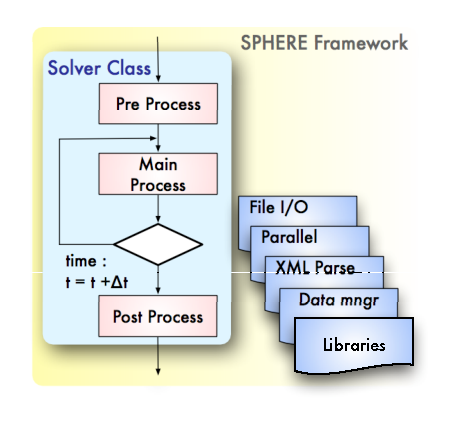
\includegraphics[width=8cm,clip]{Sphere_Control.eps}
\end{center}
\caption{V-Sphereの制御構造.プリ,メイン,ポストの処理プロセスが組み込まれており,提供されるライブラリ機能を用いてソルバークラスを構築します.}
\label{fig:Control structure}
\end{minipage} \hfill
\begin{minipage}{.47\textwidth}
\begin{center}
\includegraphics[width=7.5cm,clip]{DerivedClasses.eps}
\end{center}
\caption{差分プログラミングによるソルバークラスの開発.SklSolverBaseクラスから派生したFlowBaseクラスに共通機能をまとめ,このFBクラスを用いて目的のCBCソルバークラスを作成します.}
\label{fig:DerivedSolvers}
\end{minipage}
\end{figure}


V-Sphereの機能を用いて作成したアプリケーションはソルバークラスとしてV-Sphere自身に登録することができ,登録されたソルバークラス群は共通のユーザインターフェイスを備えたアプリケーションとして振る舞います.
\textbf{図\ref{fig:DerivedSolvers}}に示すようにSklクラス,SklBase\index{SklBase}クラス,およびSklSolverBaseクラスを提供します.
ここでは,SklSolverBaseクラスから流体解析に広く用いられる基本機能を抽出したFlowBaseクラスを作成しています.
ソルバークラスとしては,CBCクラスが派生し,さらにCBCクラスを継承してCPCソルバクラスが派生しています.
また,別の系統としてBCMソルバークラスが作成されています.
これらのソルバークラスは,例えば,シミュレートする物理現象や形状近似度,変数配置などが異なるソルバーですが,FlowBaseクラスにより統一的な振る舞いをします.
つまり,異なるソルバーであっても,ユーザーインターフェイスが統一されたアプリケーションとして構築することができます.

%
\section{CBCソルバークラス}
CBC(Cartesian based, Binary shape representation, Collocated)ソルバークラスは,V-Sphereコンポーネント群とクラスライブラリを利用して実装した非定常非圧縮性流体のソルバークラスです.
ソルバーを構築する上で必要な,パラメータハンドリング,主要な境界条件処理とパラメータの関連づけ,ファイル入出力,並列計算処理,組み込み例題など,コアアルゴリズム以外の部分は,FlowBaseクラスなどにパッケージ化しています.

CBCソルバークラスは,下記のような特徴を持っています.

\begin{description}
\item[ ] 形状近似   :キューブ近似(Binary Voxel)
\item[ ] 変数配置   :コロケート
\item[ ] 離散化    :有限体積法
\item[ ] 時間積分   :一次精度Euler陽解法%,二次精度Adams-Bashforth法,二次精度Crank-Nicolson法
\item[ ] 空間スキーム :一次精度風上,三次精度MUSCL%,二次精度中心,
\item[ ] 解法     :Fractional Step法
\item[ ] 反復法    :Jacobi緩和法, Point SOR, 2-colored SOR-SMA(ストライドメモリアクセス版)
%\item[ ]         2-colored SOR-CMA(連続メモリアクセス版)
\item[ ] スタート機能 :Initial(Impulsive, Smooth), 指定時刻からの再スタート
\item[ ] 入力ファイル :モデルファイル(svx, sbxフォーマット),XMLファイル(計算条件など)
\item[ ] 出力ファイル :sphフォーマット,履歴ファイル,モニター出力
\item[ ] 外部境界条件 :固定・移動壁面,流入,流出,周期,対称,トラクションフリー
\item[ ] 内部境界条件 :壁面,速度規定,流出,部分周期境界,圧力損失,多孔質
\item[ ] 温度境界条件 :断熱,熱伝導,熱伝達,輻射,熱流束,等温
\item[ ] 並列ライブラリ:mpich, mpich2, OpenMPI
\item[ ] 並列化    :等分割,多重連結領域分割
\item[ ] 組込み例題機能:キャビティフロー問題など,基本的な問題
\end{description}





%%%
\chapter{インストール}
\label{chpt:install}
\begin{abstract}
この章では,MPI通信ライブラリ,V-Sphere,CBCソルバークラスのインストールとコンパイルについて説明します.MPI通信ライブラリ,V-Sphereの詳細なインストールについては,V-Sphereユーザガイド(\verb|Vsphere_UG.pdf|)を,CBCソルバークラスの詳細についてはCBCソルバークラス説明書(\verb|Inside_CBC.pdf|)を参照してください.
\end{abstract}
%
%%
\section{MPIライブラリのインストール}
\label{sec:install MPI}

OpenMPI\footnote{http://www.open-mpi.org/}のインストールについて説明します.

\begin{enumerate}
\item autotoolsによるコンパイル\\
autotools~\cite{autotools}を用いて作成されたパッケージは容易にインストールができます.
典型的な場合,インストールまでの全工程が自動化され,ソースコードを展開した後,以下のコマンドを入力するだけで全てが完了します.
{\small
\begin{program}
./configure && make && make install
\end{program}
}

\item シェルスクリプトを用いたコンパイル環境の設定\\
configureのために,次のようなスクリプトを用意して実行します.
インストールディレクトリは\verb|/usr/local/openmpi|とします.
コンパイラは,Intel Compiler icpc/ifortの利用を指定しています.

{\small
\begin{program}
$ cat config_ompi.sh

#!/bin/sh
export CC=icc
export CFLAGS=-O3
export CXX=icpc
export CXXFLAGS=-O3
export F77=ifort
export FFLAGS=-O3
export FC=ifort
export FCFLAGS=-O3
#
./configure --prefix=$1

$ ./config_ompi.sh /usr/local/openmpi
\end{program}
}

\item コンパイルの実行とインストール\\
{\small
\begin{program}
$ make
$ sudo make install
\end{program}
}

\item PATHの設定\\
実行時のmpiexec\footnote{mpirunでも動きます.}が正しいパスになっているかどうかをwhichコマンドで確認します\footnote{Mac OSXの場合には上記のように,デフォルトでインストールされているOpenMPIの方を見に行くので,インストールしたOpenMPIのPATHを最初の方に書いておきます.}.

{\small
\begin{program}
$ which mpiexec
\end{program}
}

\item 環境変数の設定\\
実行時に必要な環境変数をホームディレクトリの\verb|.bash_profile|などに記述しておきます.

{\small
\begin{program}
export LD_LIBRARY_PATH=/usr/local/openmpi/lib:$LD_LIBRARY_PATH
export DYLD_LIBRARY_PATH=/usr/local/openmpi/lib:$DYLD_LIBRARY_PATH
\end{program}
}

\end{enumerate}

%
\section{V-Sphereのインストール}
\label{sec:install vsphere}
V-Sphereのインストールは,MPI通信ライブラリのインストールの後に行います.

%
\subsection{autotoolsを用いたコンパイル環境の設定}
まず,\verb|configure|の設定を行います.
次のスクリプトの例では,インストールディレクトリを\verb|/usr/local/sphere/|に指定しています.
もし,\verb|/usr/local/|領域へのアクセス権限がない場合には,各ユーザが書き込める場所を指定します.
また,LDFLAGSには,コンパイラへの適切なパスを指定します.

{\small
\begin{program}
$ cat configure.sh
$ ./configure --prefix=$1 \
              --with-comp=INTEL \
              --with-ompi=/usr/local/openmpi \
              CC=icc \
              CFLAGS=-O3 \
              CXX=icpc \
              CXXFLAGS=-O3 \
              FC=ifort \
              FCFLAGS=-O3 \
              F90=ifort \
              F90FLAGS=-O3 \
              LDFLAGS=-L/opt/intel/Compiler/11.1/089/lib/intel64
\end{program}
}

上記のインストールシェルは,引数としてインストールディレクトリを指定し,次のように実行します.
この時点で\verb|autotools|のバージョンが違う場合には以下のコマンドをV-Sphereディレクトリで実行し,環境を合わせます.

{\small
\begin{program}
$ aclocal
$ autoconf
$ automake -a
\end{program}
}

\verb|configure|により,利用者の環境を調査し,適切なコンパイル環境を設定します.

{\small
\begin{program}
$ configure.sh /usr/local/sphere
\end{program}
}

%
\subsection{モジュールの作成とインストール}
\verb|configure|の後,次のコマンドを実行します.

{\small
\begin{program}
$ make
$ sudo make install または make install
\end{program}
}

make時に\verb|libimf.so|が見つからないなどのメッセージが出る場合は,ホームディレクトリの\verb|.bash_profile|などにコンパイラのLD\_LIBRARY\_PATHパスを加えておきます.
{\small
\begin{program}
export LD_LIBRARY_PATH=/opt/intel/Compiler/11.1/089/lib:$LD_LIBRARY_PATH
\end{program}
}

%
\subsection{アンインストール}
V-Sphereをアンインストール\index{アンインストール!V-Sphereの@V-Sphereの---}する場合には,インストールしたディレクトリ(configureでオプション指定したディレクトリ:ここでは \verb|/usr/local/sphere|)の\verb|sphere|を削除します.

%
\subsection{倍精度計算モジュール}
単精度計算と倍精度計算では,それぞれ専用のV-Spghereライブラリが必要になり,単精度計算と倍精度計算で異なる精度のモジュールを別々に用意します.
倍精度計算モジュールを生成する場合には,configure時に\verb|--with-real=double|オプションを追加してください.
このオプションは,コンパイルオプションに下記のように\verb|-DREAL_IS_DOUBLE|を追加します.

{\small
\begin{program}
CFLAGS         : -O3 -DREAL_IS_DOUBLE
CXXFLAGS       : -O3 -DREAL_IS_DOUBLE
\end{program}
}

両方必要になる場合には,両方のV-Sphereライブラリを用意しておき,CBCソルバークラスのコンパイル時にリンク先を変更して,コンパイルします.


%%
\hypertarget{tgt:installCBC}{\section{CBCソルバークラスのインストールとコンパイル}}
\label{sec:install CBC}

本節では,ソルバークラスのインストールについて説明します.
提供されるソルバークラスのアーカイブ\verb|CBC_x.x.x.tar.gz|は,ソルバークラスのソースコードです\footnote{CBC\_x.x.x.tar.gzのx.x.xにはリリースバージョン番号が入ります.}.

%%
\subsection{アーカイブの解凍}
{\small
\begin{program}
$ tar xvfz CBC_x.x.x.tar.gz
\end{program}
}

解凍すると,以下のようなファイル構成になります\footnote{doxygenディレクトリについては,doxygenファイルを生成するために必要な設定ファイルのみを提供しています.Confディレクトリ内でmakeを実行すると各ディレクトリにdoxygenファイルが生成されます.}.

{ \small
\begin{program}
CBC_x.x.x
  |
  +- BUILD                        アプリケーションのコンパイル方法のメモ
  +- COPYING                      コピーライト
  +- README                       最初に見るべきファイル
  +- RELEASE                      リリース情報
  |
  +- doc                          ドキュメント
  |   +- cbc_ug.pdf               CBCソルバークラスのユーザガイド
  |   +- vsphere_ug.pdf           V-Sphereのユーザーガイド
  |   +- cbc_examples.pdf         検証の例題集
  |
  +- doxygen                      Doxygenドキュメントディレクトリ
  |   +- CBC                      CBCクラスのドキュメント
  |   +- Conf                     Doxygenファイルを生成するための設定ファイル
  |   +- FB                       FBクラスのドキュメント
  |   +- IP                       Intrinsicクラスのドキュメント
  |
  +- example                      例題
  |   +- 3Dcavity                 三次元のキャビティフロー(立方体領域)
  |   +- LDC112                   辺長1:1:2のキャビティフロー
  |   +- dragon                   ドラゴン形状周りの流れ
  |   +- Duct3D                   管路内流れ
  |   |   +- inner                ドライバ周期境界指定
  |   |   +- outer                外部周期境界指定
  |   +- PMT                      性能測定用パラメータ群
  |   +- SHC1D                    定常1次元熱伝導
  |
  +- src                          ソースコード
  |   +  F_CBC                    CBCクラスのFortranファイル
  |   +- F_CPC                    CPCクラスのFortranファイル
  |   +- F_VOF                    VOFクラスのFortranファイル
  |   +- FB                       FlowBaseクラス(ユーザー定義クラス群)
  |   +- IP                       組み込み例題クラス群
  |   +- PRJ_CBC	                 CBCプロジェクト
  |      +- app                  アプリケーションコンパイルディレクトリ
  |         ...                  他ソースファイル
  |         Makefile
  |      +- bin                  バイナリモジュール格納ディレクトリ
  |      +- CBC                  CBCソルバークラスのソースファイル
  |      |   +- CBC.xml          CBCクラスのコンパイル環境設定
  |      |      ...              他ソースファイル
  |      |      Makefile
  |      +- FB                   非ソルバークラスディレクトリ FlowBase
  |      |   +- FB.xml           FBクラスのコンパイル環境設定  
  |      |      Makefile
  |      +- IP                   非ソルバークラスディレクトリ 組み込み例題クラス群
  |      |   +- IP.xml           IPクラスのコンパイル環境設定 
  |      |      Makefile
  |      +- Makefile             アプリケーションコンパイル用 Linux/Mac
  |         PRJ_CBC.xml          CBCのコンパイル設定
  +- xsd
     CBC_xxx_FB_xxx.xsd          V-Xpitを用いたパラメータ入力の構造定義ファイル
\end{program}
}
%  |   +- Inside_CBC.pdf           CBCソルバークラスの説明書

%
\subsection{sphPrjToolを用いた簡単なインストールとコンパイル}
既に,並列ライブラリとV-Sphereが正しくインストールされていることを確認します.

まず,sphPrjToolを利用するため,環境変数\verb|SPHEREDIR|を設定します.
下記で\verb|INSTALL_DIR|はV-Sphereのインストールディレクトリを指定します.
次に,\verb|src/PRJ_CBC|ディレクトリで引数にファイル名を渡してsphPrjToolを起動し,プロジェクトのコンパイル設定を利用環境に合わせて再構築します.
localsettingsオプションを指定してresetコマンドを実行すると,sphereライブラリの\verb|config/sph-cfg.xml|に記録されているコンパイル環境情報を元にして,プロジェクト環境情報\verb|PRJ_CBC.xml|を再設定します.

{\small
\begin{program}
$ export SPHEREDIR=INSTALL_DIR
$ cd src/PRJ_CBC
$ sphPrjTool PRJ_CBC.xml
sphPrjTool> reset localsettings
sphPrjTool> print
sphPrjTool> save
sphPrjTool> quit
\end{program}
}

上記の設定の後,コンパイルを行う.

{\small
\begin{program}
$ make
\end{program}
}

%
\subsection{アンインストール}
アンインストール\index{アンインストール!SolverClassの@SolverClassの---}は,SolverClassのディレクトリごと削除します.

%
\subsection{並列計算モジュールのコンパイル}
V-Sphereは逐次計算のモジュールと並列計算のモジュールは異なるので,コンパイル時にオプションで切り替えます.
並列計算\index{へいれつけいさん@並列計算}をする場合は,\verb|PRJ_CBC.xml|内に下記の記述を追加するか,sphPrjToolを用いて設定を変更します.
デフォルトでは逐次実行モジュールになっています.

{\small
\begin{program}
$ sphPrjTool PRJ_CBC.xml
sphPrjTool> module parallel
sphPrjTool> print
sphPrjTool> save
sphPrjTool> quit
\end{program}
}

%
\hypertarget{tgt:win_compile}{\subsection{Windowsでのコンパイルと実行}}

%
\subsubsection{プロジェクトの作成}
プロジェクトツール\footnote{C:{\yen}Program Files{\yen}sphere{\yen}bin{\yen}sphPrjTool.exe}を用いWindows用のプロジェクトを作成します.
プロジェクトツールの使用については,V-Sphere\_ug.pdfを参照してください.
プロジェクトツールによって以下のMakefileが生成されます.
提供ファイルのlibxml2, zlib, iconvのインストールパスは\lq\lq C:{\yen}Program Files{\yen}ext\_libs{\yen}\rq\rq 配下になっているので注意してください.

{\small
\begin{program}
PRJ_CBC
  ├─ Makefile.win
  ├─ project_local_settings
  ├─ CBC
  │    └─ Makefile.win
  ├─ FB
  │    └─ Makefile.win
  └─ IP
       └─ Makefile.win
\end{program}
}

%
\subsubsection{コンパイル}
作成した\verb|Makefile.win|を用いてmakeを行います.
コマンドプロンプトから行うが,Visual Studioの\verb|nmake.exe|を使用するので「Visual Studio 2008 コマンド プロンプト」を起動して行います.
「Visual Studio 2008 コマンド プロンプト」は「Visual Studio 2008」―「Visual Studio Tools」メニューの配下にあります.

以下,nmakeによるコンパイルコマンドです.

{\small
\begin{program}
nmake -f Makefile.win
\end{program}
}

%
\subsubsection{CBCの実行}
ソルバの実行は必ずローカルディスクにて実行します.
ネットワークパス(ネットワークドライブ)で行うとエラーとなります\footnote{現時点 \today では原因不明です.}.

以下の設定を行います.
\begin{enumerate}
\item MPICH2のbinフォルダへパスの追加\\
並列実行ではエラーとなりませんが,逐次実行にてエラーとなります.

\item Windowsファイアウォール設定
\verb|sphere.exe|を例外へ追加します.
コントロールパネル-Windowsセキュリティセンター - Windowsファイアウォール-例外に実行を行う\verb|sphere.exe|を登録します.
\end{enumerate}


\paragraph{逐次実行方法}
次のように実行します.


{\small
\begin{program}
$ set PATH=%PATH%;C:\Program Files\MPICH2\bin
$ pwd
D:\work\CBC-1.3.0\example\3Dcavity
$ ..\..\src\PRJ_CBC\bin\sphere.exe cavity.xml
\end{program}
}


\paragraph{並列実行方法:ローカルホストにて実行}
複数のホストマシンにて実行する方法は,V-Sphere ユーザマニュアル「V-SphereUG.pdf」-11. Windows 対応(使用者向け)又はMPICH2のマニュアルを参照してください.

{\small
\begin{program}
$ pwd
D:\work\CBC-1.3.0\example\3Dcavity
$ "C:\Program Files\MPICH2\bin\mpiexec.exe" -np 4 ..\..\src\PRJ_CBC\bin\sphere.exe cavity.xml
\end{program}
}


%%
\hypertarget{tgt:win_opmi_binary}{\subsection{OpenMPIバイナリパッケージを用いたコンパイルと実行}}
OpenMPI 1.5.3よりWindowsバイナリーパッケージ\footnote{OpenMPI\_v1.5.3-2\_win32.exe}が提供されています.
OpenMPIを以下のフォルダにインストールしたと仮定して説明します.
{\small
\begin{program}
	C:\Program Files\OpenMPI
\end{program}
}

%
\paragraph{V-Sphereのコンパイル}
Config.winを変更します($\ll$で示す\verb|MPICH_DIR, MPICH_LIBS, MPICH_CFLAGS|).

{\small
\begin{program}
#
# SPHERE - Skeleton for PHysical and Engineering REsearch
#
# Copyright (c) RIKEN, Japan. All right reserved. 2004-2011
#
#

# folder settings
SPHEREDIR=C:\Program Files\sphere
INTELCXX_DIR=C:\Program Files\Intel\Compiler\C++\10.1.021\IA32
INTELFC_DIR=C:\Program Files\Intel\Compiler\Fortran\10.1.021\IA32
MSSDKS_DIR=C:\Program Files\Microsoft SDKs\Windows\v6.0A
MSVS_DIR=C:\Program Files\Microsoft Visual Studio 9.0
MPICH_DIR=C:\Program Files\OpenMPI <<

EXTLIBS_PATH=C:\Program Files\ext_libs
LIBXML2_DIR=$(EXTLIBS_PATH)\libxml2
ZLIB_DIR=$(EXTLIBS_PATH)\zlib
ICONV_DIR=$(EXTLIBS_PATH)\iconv

# flags ssettings
CFLAGS=/O3 /Qprec-div- /c /TP /MT /DWIN32 /D_WIN32 /DSKL_TIME_MEASURED /D_CATCH_BAD_ALLOC
#CXXFLAGS=/fast /c /TP /MD /DWIN32 /D_WIN32
#CXXFLAGS=/O3 /c /TP /MD /DWIN32 /D_WIN32
#CXXFLAGS=/O3 /Qipo /c /TP /MD /DWIN32 /D_WIN32
#CXXFLAGS=/O3 /Qprec-div- /c /TP /MD /DWIN32 /D_WIN32
CXXFLAGS=/O3 /Qprec-div- /c /TP /MT /DWIN32 /D_WIN32 /DSKL_TIME_MEASURED/D_CATCH_BAD_ALLOC
FCFLAGS=/O3 /Qprec-div- /c /TP /MT /DWIN32 /D_WIN32 /DSKL_TIME_MEASURED
F90FLAGS=/O3 /Qprec-div- /c /TP /MT /DWIN32 /D_WIN32 /DSKL_TIME_MEASURED

# libs settings
MPICH_LIBS= libmpi.lib <<
#XML2LIBS=libxml2.lib zlib.lib libm.lib ws2_32.lib
XML2LIBS=libxml2.lib zdll.lib libmmt.lib ws2_32.lib

# include libpath settings
INCLUDES = \
			/I"$(TOP_BUILDDIR)\include" \
			/I"$(LIBXML2_DIR)\include" \
			/I"$(ZLIB_DIR)\include" \
			/I"$(ICONV_DIR)\include"

LDFLAGS = \
		/LIBPATH:"$(INTELCXX_DIR)\lib" \
		/LIBPATH:"$(LIBXML2_DIR)\lib" \
		/LIBPATH:"$(ZLIB_DIR)\lib" \
		/LIBPATH:"$(ICONV_DIR)\lib"

MPICH_CFLAGS=/I"$(MPICH_DIR)\include" /DOMPI_IMPORTS <<
MPICH_LDFLAGS=/LIBPATH:"$(MPICH_DIR)\lib"

# exec settings
CC="$(INTELCXX_DIR)\bin\icl.exe"
CXX="$(INTELCXX_DIR)\bin\icl.exe"
FC="$(INTELFC_DIR)\bin\ifort.exe"
F90="$(INTELFC_DIR)\bin\ifort.exe"
AR="$(INTELCXX_DIR)\bin\xilib.exe"
LINK="$(INTELCXX_DIR)\bin\xilink.exe"
MANF_TOOL=mt.exe
CP=copy
RM=del /F /Q

# environments
PATH=$(MSVS_DIR)\Common7\IDE;$(MSVS_DIR)\VC\bin;$(MSSDKS_DIR)\bin;$(PATH);
INCLUDE=$(MSVS_DIR)\VC\INCLUDE;$(MSSDKS_DIR)\include;$(INCLUDE)
LIB=$(MSVS_DIR)\VC\LIB;$(MSSDKS_DIR)\lib;$(LIB)
LIBPATH=$(MSVS_DIR)\VC\LIB;$(LIBPATH)

\end{program}
}


\begin{enumerate}
\item OpenMPIのインストールパスの変更
\item \verb|libmpi.lib|の変更
\item OMPI\_IMPORTSマクロの追加
\end{enumerate}

V-Sphereをコンパイルし,作成したライブラリとインクルードファイルをC:{\yen}program files{\yen}sphere\_ompiに配置します.

{\small
\begin{program}
$ nmake /f Makefile.win
\end{program}
}

%
\paragraph{ソルバCBCのコンパイル}
\verb|project_local_settings|を変更します.\\
\verb|SPHEREDIR, MPICH_DIR, MPICH_CFLAGS, MPICH_LDFLAGS, MPICH_LIBS, SPHERE_CFLAGS, SPHERE_LDFLAGS|

{\small
\begin{program}
#
# SPHERE - Skeleton for PHysical and Engineering REsearch
#
# Copyright (c) RIKEN, Japan. All right reserved. 2004-2010
#
#
CC=gcc
CFLAGS=-g -O2
CXX="C:\Program Files\Intel\Compiler\C++\10.1.021\IA32\Bin\icl.exe"
CXXFLAGS=/O3 /Qipo /Qprec-div-
FC=f95
FCFLAGS=-g -O2
F90="C:\Program Files\Intel\Compiler\Fortran\10.1.021\IA32\Bin\ifort.exe"
F90FLAGS=/O3 /Qipo /Qprec-div-
LDFLAGS=/LIBPATH:"C:\Program Files\Intel\Compiler\Fortran\10.1.021\IA32\Lib"
LIBS=ws2_32.lib libifport.lib libmmt.lib libifcoremt.lib
SPH_USR_DEF_LIBS=
UDEF_OPT=-DNON_POLYLIB -DNON_CUTLIB
UDEF_INC_PATH=
UDEF_LIB_PATH=
UDEF_LIB_UPPER=
UDEF_LIB_LOWER=
SPHEREDIR=C:\Program Files\sphere_ompi <<
SPH_DEVICE=IA32_WIN
MPICH_DIR=C:\Program Files\OpenMPI <<
MPICH_CFLAGS=/I"C:\Program Files\OpenMPI\include" <<
MPICH_LDFLAGS=/LIBPATH:"C:\Program Files\OpenMPI\lib" <<
MPICH_LIBS=libmpi.lib <<
XML2FLAGS=/I"C:\Program Files\ext_libs\libxml2\include" /I"C:\Program Files\ext_libs\iconv\include"
XML2LIBS=libxml2.lib zdll.lib
SPHERE_CFLAGS=/DSKL_TIME_MEASURED /D_CATCH_BAD_ALLOC /I"C:\Program Files\sphere_ompi\include" <<
SPHERE_LDFLAGS=/LIBPATH:"C:\Program Files\sphere_ompi\lib" <<
SPHERE_LIBS=libsphapp.lib libsphbase.lib libsphfio.lib libsphdc.lib libsphcrd.lib libsphcfg.lib 
            libsphftt.lib libsphvcar.lib
REALOPT=
CXXFLAGS_DEF=/c /TP /MT /DWIN32 /D_WIN32
F90FLAGS_DEF=/c /MT
SPHERE_DEFINE=/DSKL_TIME_MEASURED /D_CATCH_BAD_ALLOC
ZLIB_DIR=C:\Program Files\ext_libs\zlib
ZLIB_LDFLAGS=/LIBPATH:"C:\Program Files\ext_libs\zlib\lib"
INTELCXX_DIR=
INTELF90_DIR=
LIBXML2_DIR=C:\Program Files\ext_libs\libxml2
MSSDKS_DIR=C:\Program Files\Microsoft SDKs\Windows\v6.0A
MSVS_DIR=C:\Program Files\Microsoft Visual Studio 9.0
INTELCXXBIN_DIR=C:\Program Files\Intel\Compiler\C++\10.1.021\IA32\Bin
INTELF90BIN_DIR=C:\Program Files\Intel\Compiler\Fortran\10.1.021\IA32\Bin
INTELCXXLIB_DIR=C:\Program Files\Intel\Compiler\C++\10.1.021\IA32\lib
INTELF90LIB_DIR=C:\Program Files\Intel\Compiler\Fortran\10.1.021\IA32\Lib
ICONV_DIR=C:\Program Files\ext_libs\iconv
XML2LDFLAGS=/LIBPATH:"C:\Program Files\ext_libs\libxml2\lib" 
            /LIBPATH:"C:\Program Files\ext_libs\iconv\lib"
SPH_EXTERNAL_HEADER_PATH=/I..\..\Cutlib_2_0_0\include /I..\..\FB /I..\..\F_CBC /I..\..\IP 
                         /I..\..\Polylib_2_0_2\include 
SPH_PARA_MODULE=MPI
\end{program}
}


\begin{enumerate}
\item OpenMPI用のV-Sphereのパスの変更
\item OpenMPIのインストールパスの変更
\item \verb|libmpi.lib|の変更
\end{enumerate}

ソルバCBCをコンパイルします.
{\small
\begin{program}
$ pwd
D:\work\CBC-1.3.0\src\PRJ_CBC
$ nmake -f Makefile.win
\end{program}
}

%
\paragraph{ソルバCBCの実行}
\verb|sphere.exe|を実行する前にOpenMPIへのパスを追加します.

{\small
\begin{program}
$ set PATH=%PATH%;C:\Program Files\OpenMPI\bin
\end{program}
}

ローカルホストにて,\verb|mpirun.exe|により並列実行を行います\footnote{逐次実行はエラーとなっています.}.
{\small
\begin{program}
$ pwd
D:\work\CBC-1.3.0\example\3Dcavity
$ "C:\Program Files\OpenMPI\bin\mpirun.exe" -np 4  ..\..\src\PRJ_CBC\bin\sphere.exe cavity.xml
\end{program}
}





%%%
\chapter{基礎方程式と解析方法}
\label{chpt:eqs}
\begin{abstract}
本章では,CBCソルバークラスが扱う流体の基礎方程式について簡単に説明します.詳細はCBCソルバークラス説明書(\verb|Inside_CBC.pdf|)を参照してください.
\end{abstract}
%

%
\section{支配方程式}
\label{sec:basic eqs}
CBCソルバークラスは,圧力や温度の変化により生じる流体の密度変化\index{みつどへんか@密度変化}が小さく.代表的な流速が音速に比べてかなり低い場合を仮定して,非圧縮性流体の基礎方程式を用いています.

%
\subsection{非圧縮性流体}
解析対象とする流れの特徴を以下のように仮定し,支配方程式を記述します.

\begin{itemize}
\item 流れの速度が音速に比べて十分に低く,流れの運動に対する圧縮性の影響は小さいと仮定して,流れを非圧縮性として取り扱います.
\item 温度場の代表的な温度差スケールが$30\ {}^\circ\mathrm{C}$以下で,密度変化が小さいと仮定します.この場合,密度変化が質量保存則へ与える影響は小さく,密度変化が流れの運動に及ぼす影響をBoussinesq近似\index{ぶしねきんじ@Boussinesq近似}\index{Boussinesq}によりモデル化できます.
\end{itemize}

支配方程式として,非圧縮性流れに対する質量保存則\textbf{式(\ref{eq:continuity eq})},運動量保存則\textbf{式(\ref{eq:NS eq})},エネルギー保存則\textbf{式(\ref{eq:energy eq})}を用います.
$\delta$はクロネッカーのデルタで重力方向 (i=3) のときに浮力が作用します.
ここで,プライム$[{}^{\prime}]$は有次元量を表します.物性値など有次元であることが明らかなものにはプライムは付けていません.

\begin{equation}
\frac{ \partial{{u}_{i}}^{\prime} }{ \partial{{x}_{i}}^{\prime} }\,{=}\,{0}
\label{eq:continuity eq}
\end{equation}

\begin{equation}
\rho^{\prime} \frac{\partial{{u}_{i}}^{\prime}}{\partial{t}^{\prime}} + \rho^{\prime} \frac{\partial}{\partial{{x}_{j}}^{\prime}} \left \{ \,\left( u_j^\prime - u_j^{\,g\,\prime} \right) \,u_i^\prime\,\right \}
\,{=}\,
- \frac{\partial{P}^{\prime}}{\partial{{x}_{i}}^{\prime}} + \frac{\partial}{\partial{{x}_{j}}^{\prime}} \left[ {\mu\left({ \frac{\partial{{u}_{i}}^{\prime}}{\partial{{x}_{j}}^{\prime}} + \frac{\partial{{u}_{j}}^{\prime}}{\partial{{x}_{i}}^{\prime}}} \right)} \right] - \rho^{\prime} {g}{\delta}_{i3}
\label{eq:NS eq}
\end{equation}

\begin{equation}
\rho^\prime C_p \left[ \frac{\partial \theta^\prime}{\partial t^\prime} + \frac{\partial}{\partial x_i^\prime} \left\{ \, \left( u_i^\prime - u_i^{\,g\,\prime} \right) \theta^\prime \, \right\} \right] 
\,{=}\,
\frac{D{P}^{\prime}}{D{t}^{\prime}} + \frac{\partial}{\partial{{x}_{i}}^{\prime}} \left( {\lambda \frac{\partial{\theta}^{\prime}}{\partial{{x}_{i}}^{\prime}}} \right) + \mu\Phi + {Q}^{\prime}
\label{eq:energy eq}
\end{equation}

\vspace{1.0cm}
\begin{center}
\begin{tabular}{lll}
$\rho^{\prime}$ &  $[kg\,/\,m^3]$ & density \\
$P^{\prime}$ & $[Pa]$ & pressure \\
${C}_{p}$ & $[J\,/\,(kg\,K)]$ & specific heat at constant pressure \\
$\theta^{\prime}$ & $[K]$ & temperature \\
$\lambda$ & $[W\,/\,(m\,K)]$ & heat conductivity \\
${{u}_{j}}^{\prime}$ & $[m\,/\,s]$ & velocity components \\
$u_j^{\,g\,\prime}$ & $[m\,/\,s]$ & velocity components of a grid point \\
${{x}_{j}}^{\prime}$ & $[m]$ & coordinate axis\\
$t^{\prime}$ & $[s]$ & time\\
$\mu$ & $[Pa\,s]$ & viscosity\\
$g$ & $[m\,/\,s^2]$ & gravitational acceleration\\
$\Phi$ & $[1/s^{2}]$ & dissipation function\\
$Q^{\prime}$ & $[W\,/\,m^3]$ & heat source\\
\end{tabular}
\end{center}
\vspace{1.0cm}

\noindent \textbf{式(\ref{eq:NS eq})}は形式的にALE(Arbitrary Lagrangian and Eulerian)\index{ALE}で書かれていますが,速度$u_j^{\,g\,\prime}$で移動する格子系での保存則を表現しています.格子点を固定($u_j^{\,g\,\prime}=0$)すればEuler表現,流体粒子と一緒に移動($u_j^{\,g\,\prime}=u_j^\prime$)させればLagrangian表現となります.ここでは,並進や回転などの任意の格子移動速度を与えるために$u_j^{\,g\,\prime}$を利用します.\\

\noindent 低マッハ数\index{ていまっはすう@低マッハ数}を仮定すると,散逸関数$\Phi$は$M^2$に比例するので,その寄与は小さく圧力の全微分の項の影響も小さいので,\textbf{式(\ref{eq:energy eq})}は,次のようなパッシブスカラの移流拡散方程式になります.

\begin{equation}
\frac{\partial \theta^{\prime}}{\partial{t}^{\prime}} + \frac{\partial}{\partial{{x}_{i}}^{\prime}} \left\{ \, \left( u_i^\prime - u_i^{\,g\,\prime} \right) \, \theta^\prime \, \right \}
\,{=}\, 
\frac{\partial}{\partial{{x}_{i}}^{\prime}} \left({ \mathrm{\alpha} \frac{\partial \theta^{\prime}}{\partial{{x}_{i}}^{\prime}} }\right) + \frac{Q^{\prime}}{\rho^{\prime}{C}_{p}}
\label{eq:thermal transport eq}
\end{equation}

\noindent ここで$\alpha$は温度拡散係数\index{おんどかくさんけいすう@温度拡散係数}で$[m^2/s]$の単位です.

\begin{equation}
\qquad \left.
\begin{array}{ll}
\vspace{2mm}
\alpha\,=\, \displaystyle{ \frac{\lambda}{\rho^{\prime} C_{p}} } & [m^2/s]\\
\vspace{2mm}
\nu\,=\, \displaystyle{ \frac{\mu}{\rho^{\prime}} } & [m^2s]\\
\vspace{2mm}
p\,=\, \displaystyle{ \frac{{\tilde{p}}^{\prime}}{{\rho_{0}}^{\prime}} } & [m^2/s^2]
\end{array} \quad \right\}
\label{eq:thermal transport eq2}
\end{equation}

\noindent 温度拡散係数$\alpha$が一定の場合には下記のようになります.

\begin{equation}
\frac{\partial \theta^{\prime}}{\partial{t}^{\prime}} + \frac{\partial}{\partial{{x}_{i}}^{\prime}} \left\{ \, \left( u_i^\prime - u_i^{\,g\,\prime} \right) \, \theta^\prime \, \right \} 
\,{=}\,
\mathrm{\alpha} \frac{\partial}{\partial{{x}_{i}}^{\prime}} \left({ \frac{\partial \theta^{\prime}}{\partial{{x}_{i}}^{\prime}} }\right) + \frac{Q^{\prime}} {\rho^{\prime} {C}_{p}}
\label{eq:thermal transport eq:const alpha}
\end{equation}


%
\section{無次元化}
\label{sec:non dimensionalize}
代表速度$u_0^\prime$, 代表長さ$L^\prime$, 代表温度スケール$\Delta \theta^\prime$と基準温度$\theta_0^\prime$で\textbf{式(\ref{eq:continuity eq})}, \textbf{(\ref{eq:NS eq})}, \textbf{(\ref{eq:thermal transport eq:const alpha})}を無次元化\index{むじげんか@無次元化}します.

\begin{equation}
\left.{ \begin{array}{l}
\vspace{2mm}
{u \,{=}\, \displaystyle{ \frac{ u^{\prime} } { {u_{0}}^{\prime}} } }\\
\vspace{2mm}
x \,{=}\, \displaystyle{ \frac{x^{\prime}}{L^{\prime}} }\\
\vspace{2mm}
p \,=\, \displaystyle{ \frac{p^\prime - {p_0}^\prime}{\rho^\prime {u_0^\prime}^2} }\\
\vspace{2mm}
\theta \,{=}\, \displaystyle{ \frac{\theta^{\prime} - {\theta_{0}}^{\prime}}{\Delta \theta^{\prime}} }
\end{array}\quad }\right\}
\label{eq:non dimensional basis}
\end{equation}

%
\subsection{無次元化された支配方程式}
\label{sec:natural_convection}
以下の\textbf{式(\ref{eq:continuity eq:ND})}--\textbf{(\ref{eq:thermal transport eq:ND})}は,単一成分の熱流動を表します.

\begin{equation}
\frac{\partial{u}_{i}}{\partial{x}_{i}}\,{=}\,{0}
\label{eq:continuity eq:ND}
\end{equation}

\begin{equation}
\frac{\partial{u}_{i}}{\partial{t}}{+}\frac{\partial}{\partial{x}_{j}} \left\{ \, \left( u_j - u_j^{\,g} \right) \, u_i \, \right\}
\,{=}\,
{-}\frac{\partial{p}}{\partial{x}_{i}}{+}\frac{1}{Re}\frac{\partial}{\partial{x}_{j}}\left({\frac{\partial{u}_{i}}{\partial{x}_{j}}{+}\frac{\partial{u}_{j}}{\partial{x}_{i}}}\right){+}\frac{Gr}{{Re}^{2}}{\mathrm{\delta}}_{i3}\mathrm{\theta}
\label{eq:NS eq:ND}
\end{equation}

\begin{equation}
\frac{\partial\mathrm{\theta}}{\partial{t}}{+}\frac{\partial}{\partial{x}_{i}} \left\{ \, \left( u_i - u_i^{\,g} \right) \, \mathrm{\theta} \, \right\}
\,{=}\,
\frac{1}{Pe}\frac{\partial}{\partial{x}_{i}}\frac{\partial\mathrm{\theta}}{\partial{x}_{i}}{+}\mathrm{\Theta}
\label{eq:thermal transport eq:ND}
\end{equation}

\begin{equation}
\left.{\begin{array}{l}
\vspace{2mm}
{{Re}\,{=}\,\frac{\displaystyle {{u}'}_{0}{L}'}{\displaystyle \mathrm{\nu}}}\\
\vspace{2mm}
{{Pr}\,{=}\,\frac{\displaystyle \mathrm{\mu}{C}_{p}}{\displaystyle \mathrm{\lambda}}\,{=}\,\frac{\displaystyle \mathrm{\nu}}{\displaystyle \mathrm{\alpha}}}\\
\vspace{2mm}
{{Gr}\,{=}\,\frac{\displaystyle {g}\mathrm{\beta}\mathrm{\Delta}{\mathrm{\theta}}'{{L}'}^{3}}{\displaystyle {\mathrm{\nu}}^{2}}}\\
\vspace{2mm}
{{Ra}\,{=}\,{Pr}\mathrm{\cdot}{Gr}}\\
\vspace{2mm}
{{Pe}\,{=}\,{Pr}\mathrm{\cdot}{Re}}\\
\vspace{2mm}
{\mathrm{\Theta}\,{=}\,\frac{\displaystyle Q^{\prime}}{\displaystyle {\mathrm{\rho}}'{C}_{p}}\frac{\displaystyle {L}'}{\displaystyle {{u}'}_{0}\mathrm{\Delta}{\mathrm{\theta}}'}}
\end{array}\quad }\right\}
\label{eq:ND definition}
\end{equation}

\noindent ここで,
\vspace{1.0cm}
\begin{center}
\begin{tabular}{lll}
$Pr$ & Prandtl数 & 粘性と熱の拡散率の比\\
$Re$ & Reynolds数 & 慣性力と粘性力の比\\
$Gr$ & Grashof数 & 浮力と粘性力の比\\
$Ra$ & Rayleigh数 & 不安定性のパラメータ\\
$Pe$ & Peclet数 & 対流と熱伝達のエネルギー輸送の比\\
$\Theta$ & - & 無次元の温度変化率\\
\end{tabular}
\end{center}
\vspace{1.0cm}

\noindent \textbf{式(\ref{eq:NS eq:ND})}は強制対流と自然対流を表現し,右辺第三項が自然対流と強制対流の比を表しています.
つまり,$Gr/Re^2 \gg 1$の場合には自然対流が支配的で,$Gr/Re^2 \ll 1$の場合には強制対流が支配的となります.$Gr = 0$つまり温度差が無い場合には純強制対流です.
一方,$Gr/Re^2 \rightarrow \infty$の場合には純自然対流で,流れは浮力によって駆動されるため代表速度が自明ではありません.
また,$Gr > 10^9$となるような流れは非定常性が強くなります.

\subsection{無次元化パラメータの選択}
CBCソルバーは,支配方程式を無次元化して解いています.このため,無次元化のパラメータを選択する必要がありますが,解くべき現象に応じて適切に選択します.


\subsubsection{純強制対流}
\begin{indentation}{5zw}{0zw}
\noindent \textbf{式(\ref{eq:NS eq:ND})}においては$\,Gr=0\,$なので$\,Re\,$が支配パラメータとなります.
無次元化のスケーリングは,$\,{u_{0}}^{\prime},\,L^{\prime},\,\nu,\,\,\alpha\,(\,=\lambda / \rho^{\prime} C_{p})\,$を与えます.\\

\end{indentation}

\subsubsection{熱対流}
\begin{indentation}{5zw}{0zw}
\paragraph{浮力の効果を考慮しない場合}
\noindent \textbf{式(\ref{eq:NS eq:ND})}において,純強制対流と同じく$\,Gr=0\,$です.\textbf{式(\ref{eq:thermal transport eq:ND})}では$Pe\,$が支配パラメータとなります.
無次元化のスケーリングは,$\,{u_{0}}^{\prime},\,L^{\prime},\,\nu,\,\,\alpha\,(\,=\lambda / \rho^{\prime} C_{p})\,$を与えます.\\
\paragraph{浮力の効果を考慮する場合}
\textbf{式(\ref{eq:NS eq:ND})}では$\,Gr,\,Re\,$が,\textbf{式(\ref{eq:thermal transport eq:ND})}では$\,Pe\,$が支配パラメータとなります.
無次元化のスケーリングは,$\,{u_{0}}^{\prime},\,L^{\prime},\,\Delta\theta^{\prime},\,\beta,\,g,\,\nu,\,\alpha,\,Pr\,$を与えます.\\
\end{indentation}

\subsubsection{純自然対流}
\begin{indentation}{5zw}{0zw}
\noindent 浮力の効果を考慮した熱対流と同じでです.ただし,${u_{0}}^{\prime}$は自明でないので,純自然対流の場合の代表流速はスケールアナリシスから推測され\cite{nakayama:02:netsuryuutai},$Pr$数が小さい場合は次式のように見積もることができます.

\begin{equation}
u_{\mathit 0}^\prime \, = \, \sqrt{g \beta \Delta \theta^\prime L^\prime}
\label{eq:scaling natural u_ref}
\end{equation}

\noindent 自然対流の場合の代表速度は\textbf{式(\ref{eq:scaling natural u_ref})}の関係を用いて見積もり,代表速度パラメータとして与えます.
自然対流と強制対流が共存する共存対流の場合には,各々の代表スケールの平均値や大きい方の値を代表速度とします.\\

\end{indentation}

\subsubsection{固体熱伝導}
\begin{indentation}{5zw}{0zw}
\noindent \textbf{式(\ref{eq:thermal transport eq:ND})}の形式で$\,Pe\,$が支配パラメータとなります.ただし,対流項の寄与はありません.
無次元化のスケーリングは,$\,L^{\prime},\,\Delta \theta^{\prime},\,\alpha,\,$を与えます.
$\,{u_{0}}^{\prime}$には,一般に熱輸送の時間スケールと代表速度は熱流の伝播速度に相当すると考え,次式を用います.

\begin{equation}
{u_{\mathit{0}}}^{\prime} \,= \,\frac{\alpha}{L^{\prime}}
\label{eq:velocity scale in natural convection}
\end{equation}\\
\end{indentation}

%%
\begin{comment}
\subsubsection{共役熱移動}
\begin{indentation}{5zw}{0zw}
\noindent 共役熱移動は,固体中の熱移動と流体中の熱流動を同時に扱うので,必然的に多媒質の熱移動問題となります.熱流動は浮力効果を考慮しています.
%式(\ref{eq:NS eq:ND})では$\,Gr,\,Re$,式(\ref{thermal transport eq:ND})では$Pe\,$が支配パラメータとなる.無次元化のスケーリングは,$\,L^{\prime},\,\Delta\theta^{\prime},\,\beta,\,g,\,\nu,\,\alpha,\,Pr,\,$を与え,適切な$\,{u_{0}}^{\prime}$を用いる.\\
\end{indentation}
\end{comment}
%%

%
\section{解法アルゴリズム}
\label{sec:Algorithm NS}
この節では前節の支配方程式に対して,非圧縮性流体の解法に使われる分離解法\index{ぶんりかいほう@分離解法}を適用し,有限体積法で離散化する.

\subsection{Fractional Step法}
\label{sec:fractional step}
非圧縮性のNavier-Stokes方程式\textbf{(\ref{eq:NS eq:ND})}の解法として,Fractional step法\index{Fractional step}を用いる.これは,任意のベクトル場が非回転場と湧き出し無しの直交するベクトル場に分解できる性質を利用して,二つのベクトルの和をとることにより解を求める分離解法である.

離散式のコーディングポリシーとして,各セル単位で計算を進めていく.保存的な支配方程式を解くのでセル界面の流束ベースの評価が素直で演算量も少なくなるが,コロケートでは固体面や境界面の処理を考える上でセル単位毎の方が計算処理がしやすい.

%
\subsubsection{Euler Explicit}
\begin{indentation}{5zw}{0zw}
一次精度の時間進行法である.

\paragraph{Navier-Stokes equations} $\mbox{}$\\
\textbf{式(\ref{eq:NS eq:ND})}の対流項と粘性項をそれぞれ$C_i,\,D_i$,浮力項を外力$f_i$で表すと,

\begin{equation}
\left.
\begin{array}{l}
\vspace{2mm}
\displaystyle{ \frac{\partial u_i}{\partial t} + C_i \,=\, - \frac{\partial p}{\partial x_i} + D_i + f_i } \\
\vspace{2mm}
\qquad \displaystyle{ C_i \,=\, \frac{\partial}{\partial x_j} \left\{ \, \left( u_j - u_j^{\,g} \right) \, u_i \, \right\} } \\
\vspace{2mm}
\qquad \displaystyle{ D_i \,=\, \frac{1}{Re}\frac{\partial}{\partial x_j} \left( \frac{\partial u_i}{\partial x_j} + \frac{\partial u_j}{\partial x_i} \right) } \\
\vspace{2mm}
\qquad \displaystyle{ f_i \,=\, \frac{Gr}{{Re}^2} \delta_{i3} \theta } \\
\end{array} \quad \right \}
\label{eq:NS eq CDf}
\end{equation}

\noindent 疑似ベクトルの予測式は,
\begin{equation}
u_i^{\,*} \,=\, u_i^{\,n} + \Delta t \left( D_i^{\,n} - C_i^{\,n} + f_i^{\,n} \right)
\label{eq:pseudo vector EE}
\end{equation}

\noindent 連続の式による拘束条件から,圧力のPoisson方程式は,
\begin{equation}
\frac{\partial}{\partial x_i} {\frac{\partial p}{\partial x_i}}^{n+1}
\,=\,
\frac{1}{\Delta t} {\frac{\partial \bar{u}_i}{\partial x_i}}^* \vspace{1mm}
\label{eq:Poisson eq}
\end{equation}

\noindent 圧力ポテンシャルによるセルセンターとスタガード位置の速度ベクトルの修正式は,
\begin{equation}
u_i^{\,n+1} \,=\, u_i^{\,*} - \Delta t {\frac{\partial p}{\partial x_i}}^{n+1}
\label{eq:Pressure correction CC}
\end{equation}

\begin{equation}
u_{i,\,face}^{\,n+1} \,=\, \bar{u}_{i,\,face}^{\,*} - \Delta t {\frac{\partial p}{\partial x_i}}^{n+1}
\label{eq:Pressure correction CF}
\end{equation}

\paragraph{Thermal transport equation} $\mbox{}$\\
\textbf{式(\ref{eq:thermal transport eq:ND})}の移流項と拡散項をそれぞれ$Cs_i,\,Ds_i$で表すと,

\begin{equation}
\left.
\begin{array}{l} 
\vspace{2mm}
\displaystyle { \frac{\partial \theta}{\partial t} + Cs_i \,=\, Ds_i + \Theta } \\
\vspace{2mm}
\qquad \displaystyle{ Cs_i \,=\, \frac{\partial}{\partial x_i} \left\{ \, \left( u_i - u_i^{\,g} \right) \, \theta \, \right\} } \\
\vspace{2mm}
\qquad \displaystyle{ Ds_i \,=\, \frac{1}{Pe}\frac{\partial}{\partial x_i} \frac{\partial \theta}{\partial x_i} } \\
\end{array} \quad \right \}
\label{eq:thermal transport eqs}
\end{equation}

\begin{equation}
\theta^{\,n+1} \,=\, \theta^{\,n} + \Delta t \left( Ds_i^{\,n} - Cs_i^{\,n} + \Theta^{\,n} \right)
\label{eq:thermal transport EE}
\end{equation}

\end{indentation}

%
\begin{comment}
\subsubsection{Adams-Bashforth}
\begin{indentation}{5zw}{0zw}
二次精度ではあるが,安定条件が厳しい.

\paragraph{Navier-Stokes equations}
\begin{equation}
u_i^{\,*} \,=\, u_i^{\,n} + \Delta t \left[ \frac{1}{2} \left\{  3 \left( D_i^{\,n} - C_i^{\,n} \right)
               - \left( D_i^{\,n-1} - C_i^{\,n-1} \right) \, \right\} + \frac{1}{2} \left( 3f_i^{\,n} - f_i^{\,n-1} \right) \, \right]
\label{eq:pseudo vector AB}
\end{equation}

\paragraph{Thermal transport equation}
\begin{equation}
\theta^{\,n+1} \,=\, \theta^{\,n} + \Delta t \left[ \frac{1}{2} \left\{ 3\left( Ds_i^{\,n}- Cs_i^{\,n} \right) - \left( Ds_i^{\,n-1}- Cs_i^{\,n-1} \right) \right\} + \frac{1}{2} \left( 3\Theta^{\,n} -\Theta^{\,n-1} \right) \, \right]
\label{eq:thermal transport AB}
\end{equation}

\end{indentation}

%
\subsubsection{Adams-Bashforth + Crank-Nicolson}
\begin{indentation}{5zw}{0zw}
拡散項に由来する安定条件による時間積分幅の制限を緩和するため,陰解法を導入する.

\paragraph{Navier-Stokes equations}
\begin{equation}
u_i^{\,*} \,=\, u_i^{\,n} + \Delta t \left[ - \frac{1}{2} \left(  3 C_i^{\,n} - C_i^{\,n-1} \right)
               + \frac{1}{2} \left( D_i^{\,n} + D_i^{\,*}  \right) + \frac{1}{2} \left( 3f_i^{\,n} - f_i^{\,n-1} \right) \, \right]
\label{eq:pseudo vector ABCN}
\end{equation}

\noindent 実装は,

\begin{equation}
\left.
\begin{array}{l}
\vspace{2mm}
\displaystyle{ \bar{u}_i \,=\, u_i^{\,n} \,+\, \Delta t \left[ - \frac{1}{2} \left(  3 C_i^{\,n} - C_i^{\,n-1} \right)
+ \frac{1}{2} D_i^{\,n} + \frac{1}{2} \left( 3f_i^{\,n} - f_i^{\,n-1} \right) \, \right] } \\
\vspace{2mm}
\displaystyle{ u_i^* \,=\, \bar{u}_i \,+\, \frac{\Delta t}{2} \bar{D} }\\
\vspace{2mm}
\displaystyle{ u_{\,i,j,k}^* \,=\, \bar{u}_{\,i,j,k} \,+\, \frac{\Delta t}{2\,Re\,h^2} \left( \sum \limits_l {u_{\,l}^*} - 6\,u_{\,i,j,k}^* \right) } \\
\vspace{2mm}
\displaystyle{ \left( 1 + \frac{3\,\Delta t}{Re\,h^2} \right) u_{\,i,j,k}^* \,=\, \bar{u}_{\,i,j,k} + \frac{\Delta t}{2\,Re\,h^2} \sum \limits_l {u_{\,l}^*} } \\
\end{array} \quad \right\}
\label{eq:CN iteration ABCN}
\end{equation}

\paragraph{Thermal transport equation}
\begin{equation}
\theta^{\,n+1} \,=\, \theta^{\,n} + \Delta t \left[ - \frac{1}{2} \left( 3 Cs_i^{\,n} - Cs_i^{\,n-1} \right) + 
\frac{1}{2} \left( Ds_i^{\,n} + Ds_i^{\,n+1}\right) + \frac{1}{2} \left( 3\Theta^{\,n} -\Theta^{\,n-1} \right) \, \right]
\label{eq:thermal transport ABCN}
\end{equation}

\noindent 実装は,

\begin{equation}
\left.
\begin{array}{l}
\vspace{2mm}
\displaystyle{ \bar{\theta} \,=\, \theta^{\,n} + \Delta t \left[ - \frac{1}{2} \left( 3 Cs_i^{\,n} - Cs_i^{\,n-1} \right) + 
\frac{1}{2} Ds_i^{\,n} + \frac{1}{2} \left( 3\Theta^{\,n} -\Theta^{\,n-1} \right) \, \right] } \\
\vspace{2mm}
\displaystyle{ \theta^{\,n+1} \,=\, \bar{\theta} + \frac{\Delta t}{2} Ds_i^{\,n+1} } \\
\vspace{2mm}
\displaystyle{ \theta_{\,i,j,k}^{\,n+1} \,=\, \bar{\theta}_{\,i,j,k} + \frac{\Delta t}{2\,Pe\,h^2} \left( \sum \limits_l {\theta_{\,l}^{\,n+1}} - 6\,\theta_{\,i,j,k}^{\,n+1} \right) } \\
\vspace{2mm}
\displaystyle{ \left( 1 + \frac{3\,\Delta t}{Pe\,h^2} \right) \theta_{\,i,j,k}^{\,n+1} \,=\, \bar{\theta}_{\,i,j,k} + \frac{\Delta t}{2\,Pe\,h^2} \sum \limits_l {\theta_{\,l}^{\,n+1}} } \\
\end{array} \quad \right\}
\label{eq:CN iteration ABCN thermal}
\end{equation}

\end{indentation}

%
\subsubsection{Runge-Kutta + Crank-Nicolson}
\begin{indentation}{5zw}{0zw}
二次精度の時間進行法,対流項には2段階Runge-Kutta法\index{Runge-Kutta},拡散項にはCrank-Nicolson法\index{Crank-Nicolson}を用いる.

\paragraph{1st step : Predictor} $\mbox{}$\\
積分幅を$\Delta t/2$にとりEuler陽解法で時間積分し,n+1/2タイムレベルでの予測値を得る.

\subparagraph{Navier-Stokes equations}

\begin{equation}
u_i^{\,*,\,n+1/2} \,=\, u_i^{\,n} + \frac{\Delta t}{2} \left( D_i^{\,n} - C_i^{\,n} + f_i^{\,n} \right) \vspace{2mm}
\label{eq:pseudo vector RKCN predictor}
\end{equation}

$n+1/2\,$タイムレベルの圧力Poisson式
\begin{equation}
\frac{\partial}{\partial x_i} {\frac{\partial p}{\partial x_i}}^{n+1/2}
\,=\,
\frac{2}{\Delta t} {\frac{\partial u_i}{\partial x_i}}^{*,\,n+1/2} \vspace{2mm}
\label{eq:Poisson RKCN predictor}
\end{equation}

$n+1/2\,$タイムレベルの圧力ポテンシャルによる速度の修正式
\begin{equation}
u_i^{\,n+1/2} \,=\, u_i^{\,*,\,n+1/2} - \frac{\Delta t}{2} {\frac{\partial p}{\partial x_i}}^{n+1/2} \vspace{2mm}
\label{eq:1st Pressure correction RKCN predictor}
\end{equation}

\subparagraph{Thermal transport equation}

\begin{equation}
\theta^{\,n+1/2} \,=\, \theta^{\,n} + \frac{\Delta t}{2} \left( Ds_i^{\,n} - Cs_i^{\,n} + \Theta^{\,n} \right)
\label{eq:thermal transport RKCN predictor}
\end{equation}


\paragraph{2nd step : Corrector}
\subparagraph{Navier-Stokes equations} $\mbox{}$\\
$u^{\,*,\,n+1}$について反復的に解く.
\begin{equation}
u_i^{\,*,\,n+1} \,=\, u_i^{\,n} + \Delta t \left\{ \frac{1}{2} \left( D_i^{\,n} + D_i^{\,*,\,n+1} \right) - C_i^{\,n+1/2} + f_i^{\,n+1/2} \right\} \vspace{2mm}
\label{eq:pseudo vector RKCN corrector}
\end{equation}


\begin{equation}
\frac{\partial}{\partial x_i} {\frac{\partial p}{\partial x_i}}^{n+1}
\,=\,
\frac{1}{\Delta t} {\frac{\partial u_i}{\partial x_i}}^{*,\,n+1}
\label{eq:Poisson RKCN corrector}
\end{equation}

\begin{equation}
u_i^{\,n+1} \,=\, u_i^{\,*,\,n+1} - \Delta t {\frac{\partial p}{\partial x_i}}^{n+1} \vspace{1mm}
\label{eq:Pressure correction RKCN corrector}
\end{equation}


\subparagraph{Thermal transport equation} $\mbox{}$\\
拡散項にCrank-Nicolson法\index{Crank-Nicolson}を用いると,

\begin{equation}
\theta^{\,n+1} \,=\, \theta^{\,n} + \Delta t \left\{ \frac{1}{2} \left( Ds_i^{\,n} + Ds_i^{\,n+1} \right) - Cs_i^{\,n+1/2} + \Theta^{\,n+1/2} \right\}
\label{eq:thermal transport RKCN corrector2}
\end{equation}

\noindent 一方,拡散項にもRunge-Kuttaスキームを用いる場合には,次のようになる.

\begin{equation}
\theta^{\,n+1} \,=\, \theta^{\,n} + \Delta t \left( Ds_i^{\,n+1/2} - Cs_i^{\,n+1/2} + \Theta^{\,n+1/2} \right)
\label{eq:thermal transport RKCN corrector1}
\end{equation}

\end{indentation}

\end{comment}



%%%
\chapter{解析モデルの作成}
\label{chpt:model}
\begin{abstract}
この章では,解析モデルの作成方法を説明します.解析モデルの作成については,2種類の方法があります.まず最初にSTLやOBJなどのフォーマットの形状データを基に,ボクセル作成アプリケーションV-Xgenで行う解析モデルの作成法について説明します.次に,組み込み例題を用いたモデルの扱いについて説明します.
\end{abstract}
%

\graphicspath{{./fig_Model/}}

%
\section{形状近似度による解析モデルの分類}
\label{sec:classification of model}
直交格子を用いる流体解析では,解析対象となる形状を直交格子上でどのように扱うかにより,計算のロバスト性,予測精度,計算時間,計算格子(解析モデル)の作りやすさなどの特性が異なります.一般には,\textbf{図\ref{fig:class model}}のように分類することができます\cite{CFDハンドブック:03}.

\begin{figure}[htdp]
\begin{center}
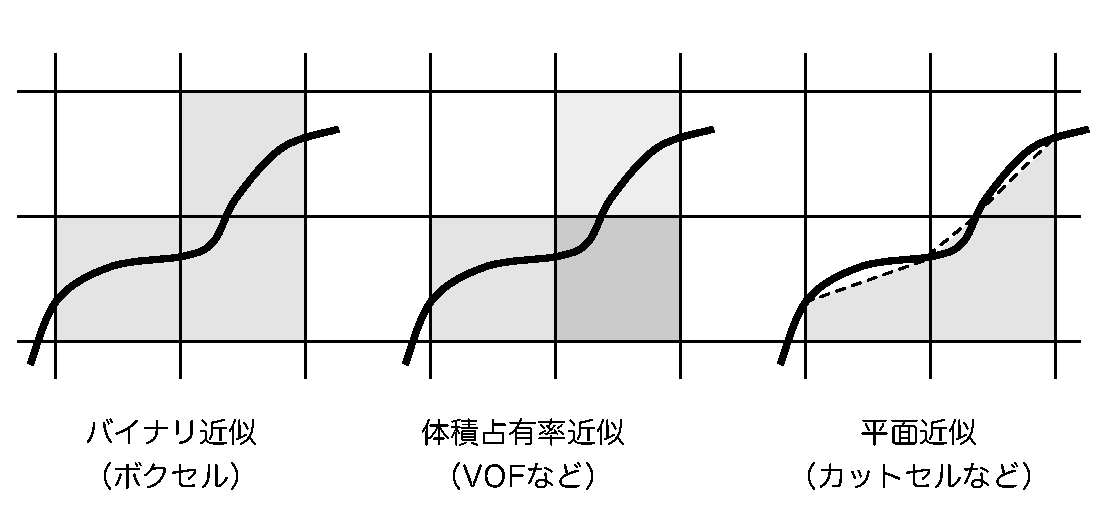
\includegraphics[width=11cm,clip]{classification.eps}
\caption{直交格子における形状近似度の分類}
\label{fig:class model}
\end{center}
\end{figure}

%
\subsection{Binary Voxel}
\label{sec:binary voxel}
Binary Voxel\index{Binary Voxel}モデルは,\textbf{図\ref{fig:Eport binary voxel}}に示すように立方体のセル要素単位で形状を表現する解析モデルです.
物体の形状近似としては最も簡単であり,モデル作成時のロバスト性に大きな利点があります.

\begin{figure}[htbp]
\begin{minipage}{.6\textwidth}
\begin{center}
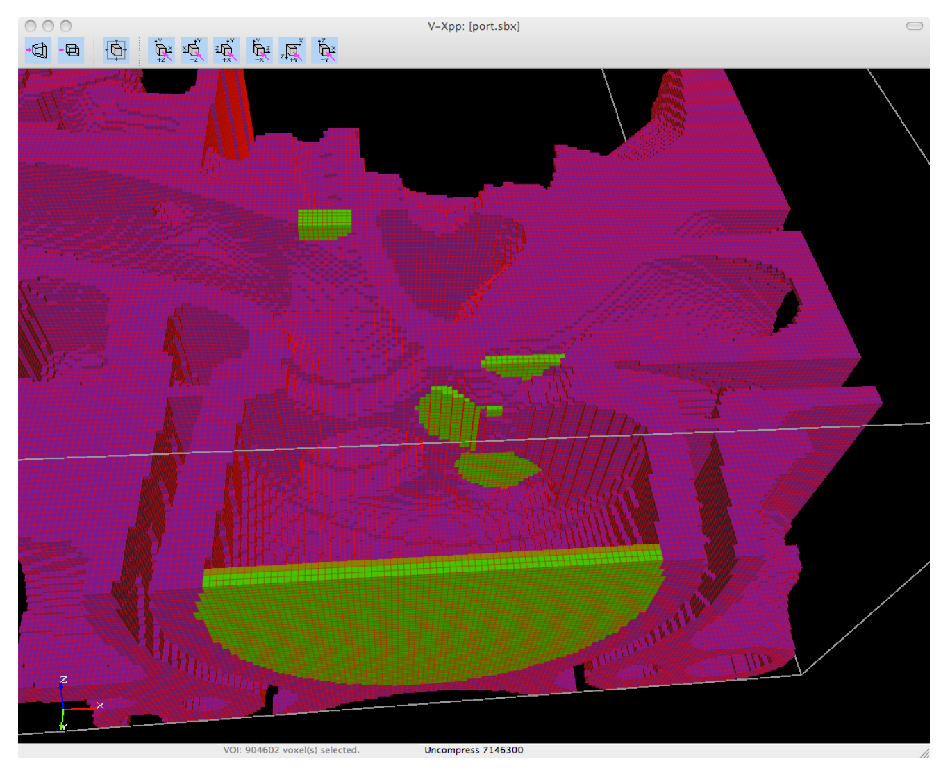
\includegraphics[width=8cm,clip]{eport.eps}
\end{center}
\caption{バイナリボクセルによる機械部品の形状表現とセルID設定}
\label{fig:Eport binary voxel}
\end{minipage} \hfill
\begin{minipage}{.38\textwidth}
\begin{center}
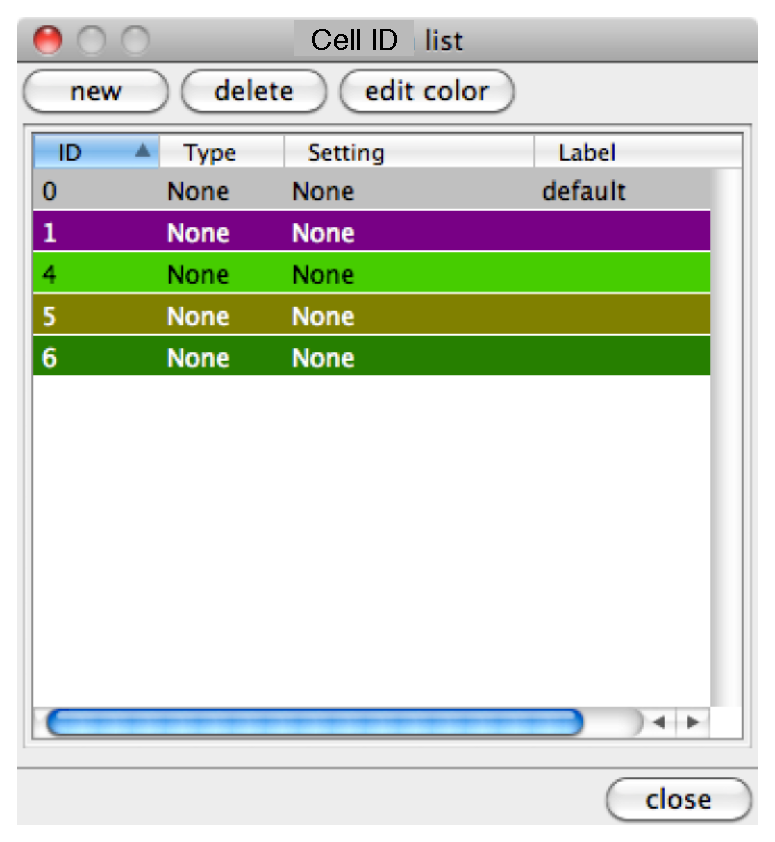
\includegraphics[width=6cm,clip]{Mlist.eps}
\end{center}
\caption{V-XgenでのセルID設定リスト}
\label{fig:ID set on V-Xgen}
\end{minipage}
\end{figure}

%
\subsection{体積率モデル}
Binary Voxelの形状近似度を改善する方法の一つで,セル内における流体の占有率を考慮した計算をする場合に利用します.
陽的な面の情報をもたないので,界面は拡散的に表現される傾向です.補助的に面における開口率を用いる場合には,有限体積法との親和性が高く保存性が改善されます.
%
\subsection{カットモデル}
\label{sec:planar cut}
Binary Voxelでは形状が階段状に近似されるため,計算精度が不足する場合があります.そこで,形状を区分的にカットされた平面として近似するモデルを用います.
CPCソルバー\footnote{\today 未実装.}では,物理量の定義点から物体までの距離情報を用いることにより,ロバスト性と精度向上の両立を図っています.通常のボクセルについてはバイナリボクセルと同様です.


%
\section{セルIDによる境界条件の指定}
\label{sec:ID connection}

CBC/CPCソルバーでは,ボクセルの各セルにIDを与え,このセルIDとパラメータファイルに記述された境界条件情報から,境界条件を設定するしくみになっています.
例えば,ボクセルモデルのセルIDとXML記述のパラメータファイル中では,次のように媒質IDと結びつけられます.

{\small
\begin{program}
<Elem name="Model_Setting">
  <Param name="fluid" id="1"   dtype="INT" value="100" comment="air"/>
  <Param name="solid" id="600" dtype="INT" value="600" comment="wall"/>
  <Param name="solid" id="610" dtype="INT" value="600" comment="piston_head"/>
</Elem>
\end{program}
}

\noindent ここでは,流体であるセルID=1は媒質ID=100によりその物性値が定義され,airのコメントがつけられています.
参照される媒質IDは,Medium\_Tableタグによって次のように指定されます.

{\small
\begin{program}
<Medium_Table>
  <Elem name="Fluid" id="100" comment="Air">
    <Param name="density"              dtype="REAL" value="1.1763" />
    <Param name="specific_heat"        dtype="REAL" value="1007" />
    <Param name="thermal_conductivity" dtype="REAL" value="2.614e-02" />
    <Param name="kinematic_viscosity"  dtype="REAL" value="15.83e-06" />
    <Param name="viscosity"            dtype="REAL" value="18.62e-06" />
    <Param name="sound_of_speed"       dtype="REAL" value="340.0" />
  </Elem>
  <Elem name="Solid" id="600" comment="Fe">
    <Param name="density"              dtype="REAL" value="7870.0" />
    <Param name="specific_heat"        dtype="REAL" value="442.0" />
    <Param name="thermal_conductivity" dtype="REAL" value="80.3" />
  </Elem>
</Medium_Table>
\end{program}
}

媒質IDの指定についての詳細は,\hyperlink{tgt:medium_table}{Medium\_Table}セクションを参照してください.

\pagebreak
%
\section{形状データからの解析モデルの作成手順}
\label{sec:modeling procedure}
V-Xgen\index{V-Xgen}を用いた解析モデル作成の手順を簡単に示します.操作の詳細は,V-Xgenユーザーガイド,およびチュートリアルを参照してください.

\begin{enumerate}
\item V-Xgenの起動\\
アイコンのダブルクリック,または下記のようにコマンドラインからアプリケーションを起動します.

{\small
\begin{program}
$ Vxgen.sh または Vxgen
\end{program}
}

\item ファイルの読み込み\\
入力となる幾何形状STLファイル\index{STL}を読み込みます.
\verb|File > Import > Shape (obj/stl) data files...|のコマンドを実行し,ファイルリストから幾何形状ファイルを選択しロードすると,\textbf{図\ref{fig:V-Xgen mesh}}のように形状モデルが描画されます.\\

\begin{figure}[htbp]
\begin{minipage}{.6\textwidth}
\begin{center}
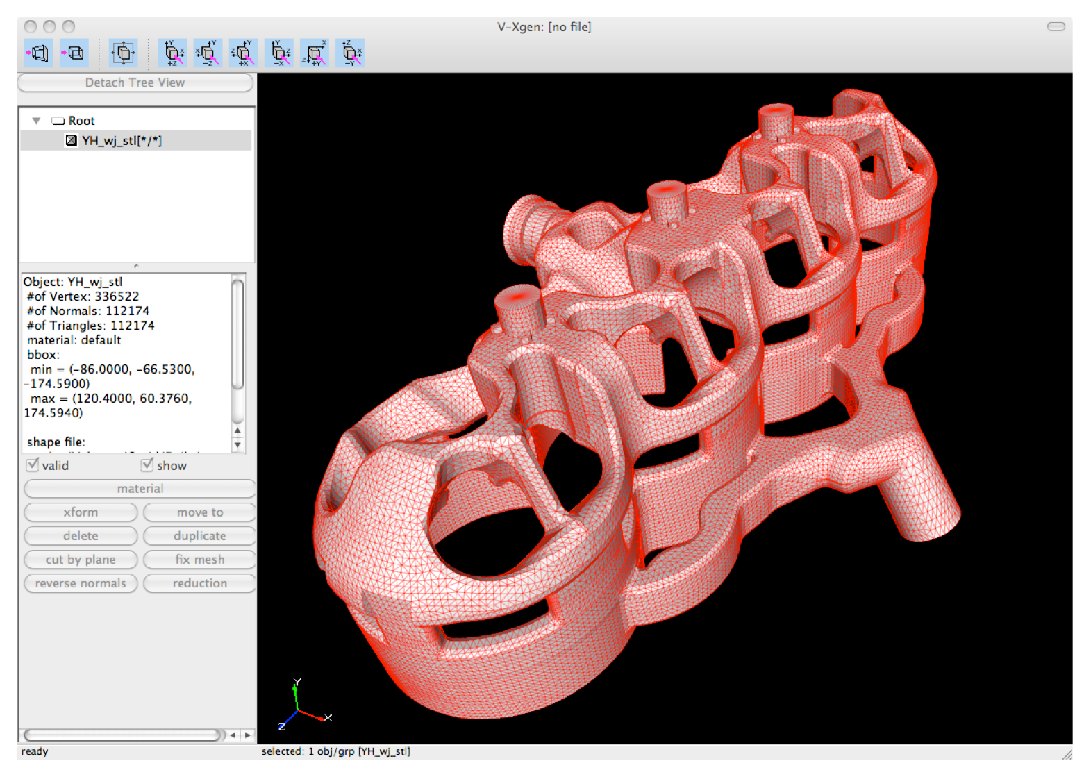
\includegraphics[width=8.5cm,clip]{WJ_mesh.eps}
\end{center}
\caption{V-Xgenでのファイル読み込み}
\label{fig:V-Xgen mesh}
\end{minipage} \hfill
\begin{minipage}{.38\textwidth}
\begin{center}
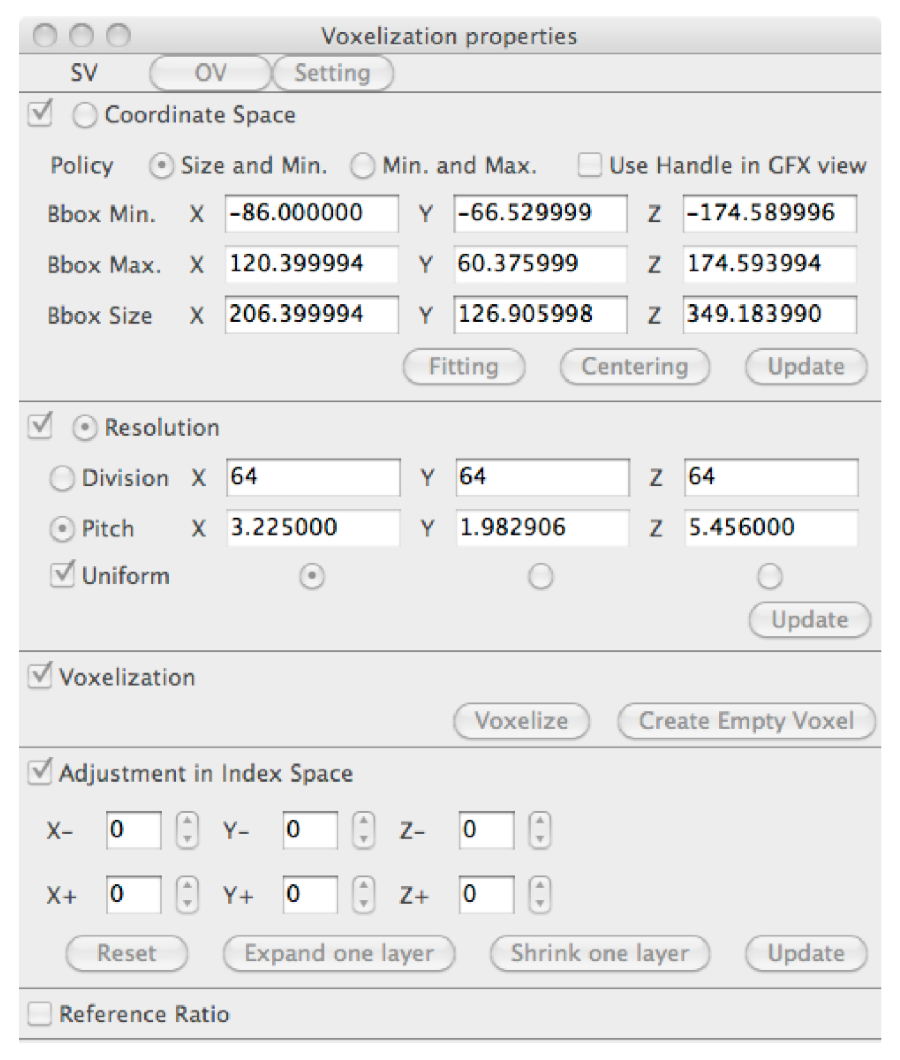
\includegraphics[width=6cm,clip]{SV_dialog.eps}
\end{center}
\caption{ボクセル作成のパラメータ設定ダイアログ}
\label{fig:SV menue}
\end{minipage}
\end{figure}

\item バイナリボクセルの作成\\
\verb|Voxelization > Simple Voxel(SV) ...|を実行すると,\textbf{図\ref{fig:SV menue}}のような直交等間隔ボクセルを作成するダイアログが表示されます.
パラメータを適切に設定して,ボクセルを作成すると,\textbf{図\ref{fig:V-Xgen voxelize}}のようなボクセルのバウンディングボックスが表示されます.
ここで作成するボクセルモデルの範囲は,\textbf{図\ref{fig:cal. region}}に示す計算領域の部分です.
計算に必要な計算領域の外部に位置する仮想セル領域の媒質はXMLパラメータファイルのOuterBoundary$\to$Face\_BC中のCell\_IDタグで指定します.\\

\begin{figure}[htbp]
\begin{minipage}{.48\textwidth}
\begin{center}
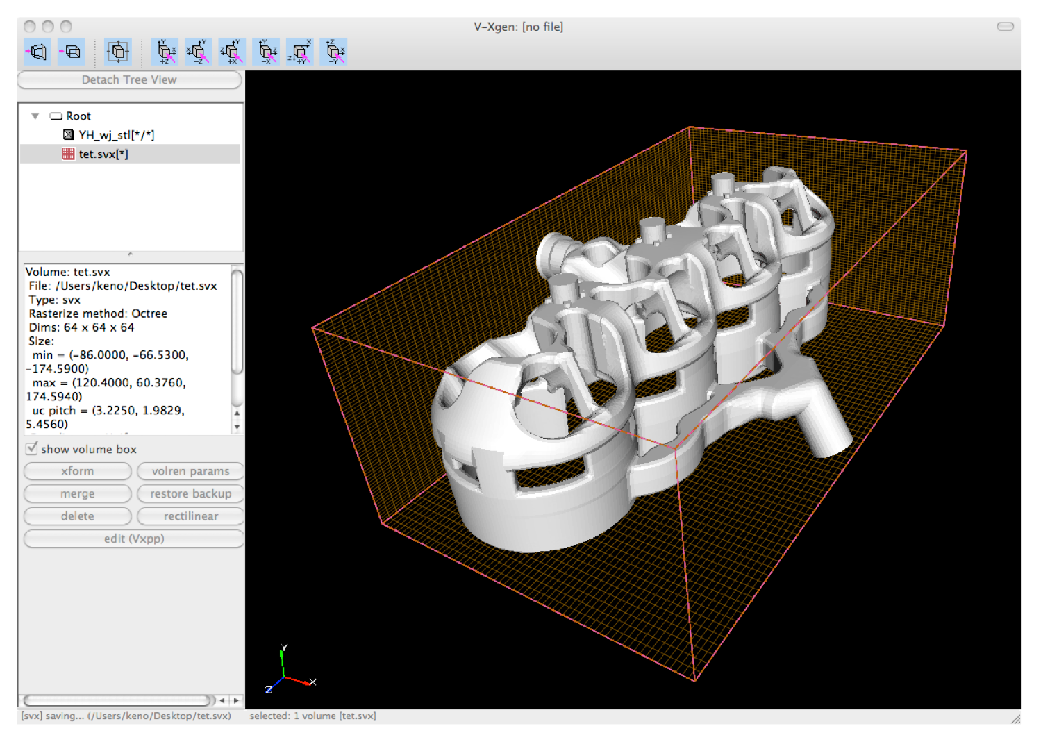
\includegraphics[width=8cm,clip]{voxelize.eps}
\end{center}
\caption{V-Xgenでのボクセル生成}
\label{fig:V-Xgen voxelize}
\end{minipage} \hfill
\begin{minipage}{.48\textwidth}
\begin{center}
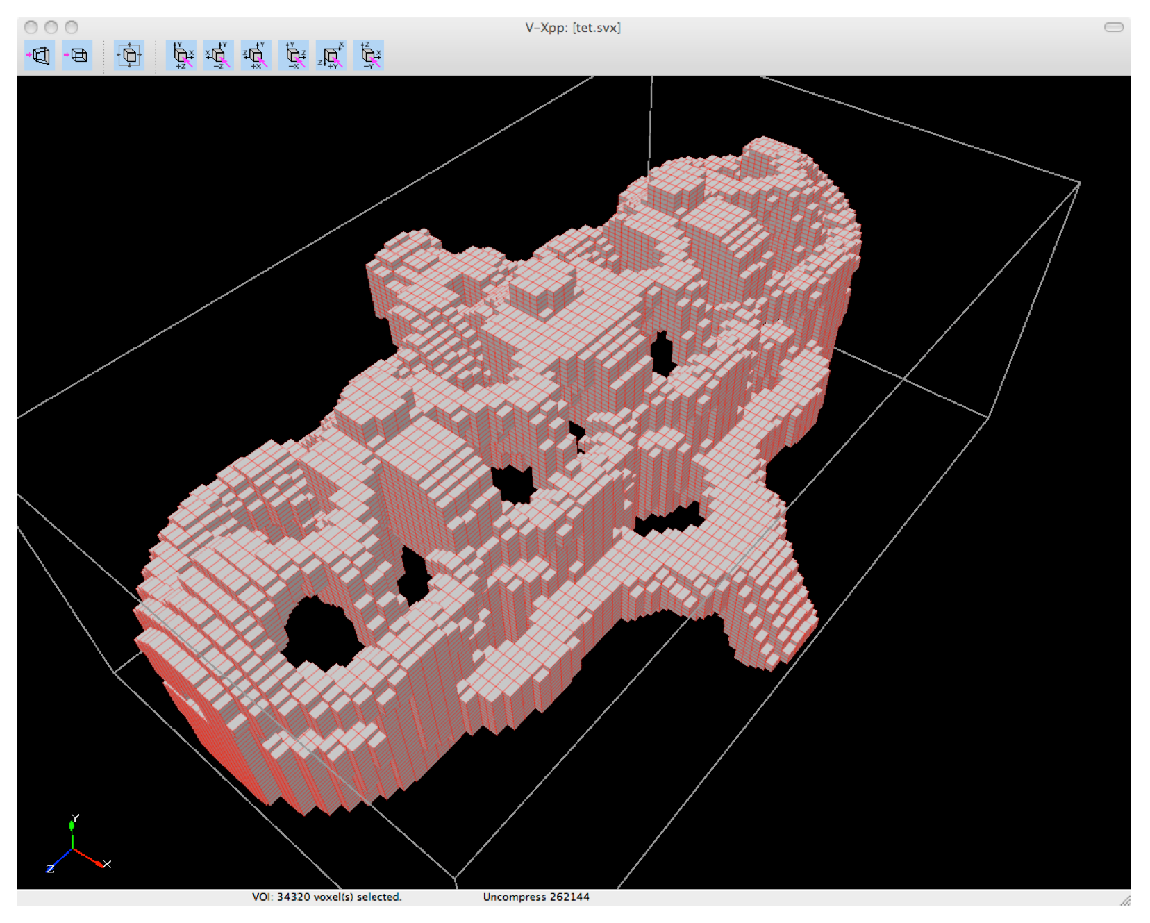
\includegraphics[width=7cm,clip]{WJ_voxel.eps}
\end{center}
\caption{ボクセルモデル.V-XppのVOIコマンドによる選択状態の表示}
\label{fig:V-Xpp voxel}
\end{minipage}
\end{figure}

\begin{figure}[htdp]
\begin{center}
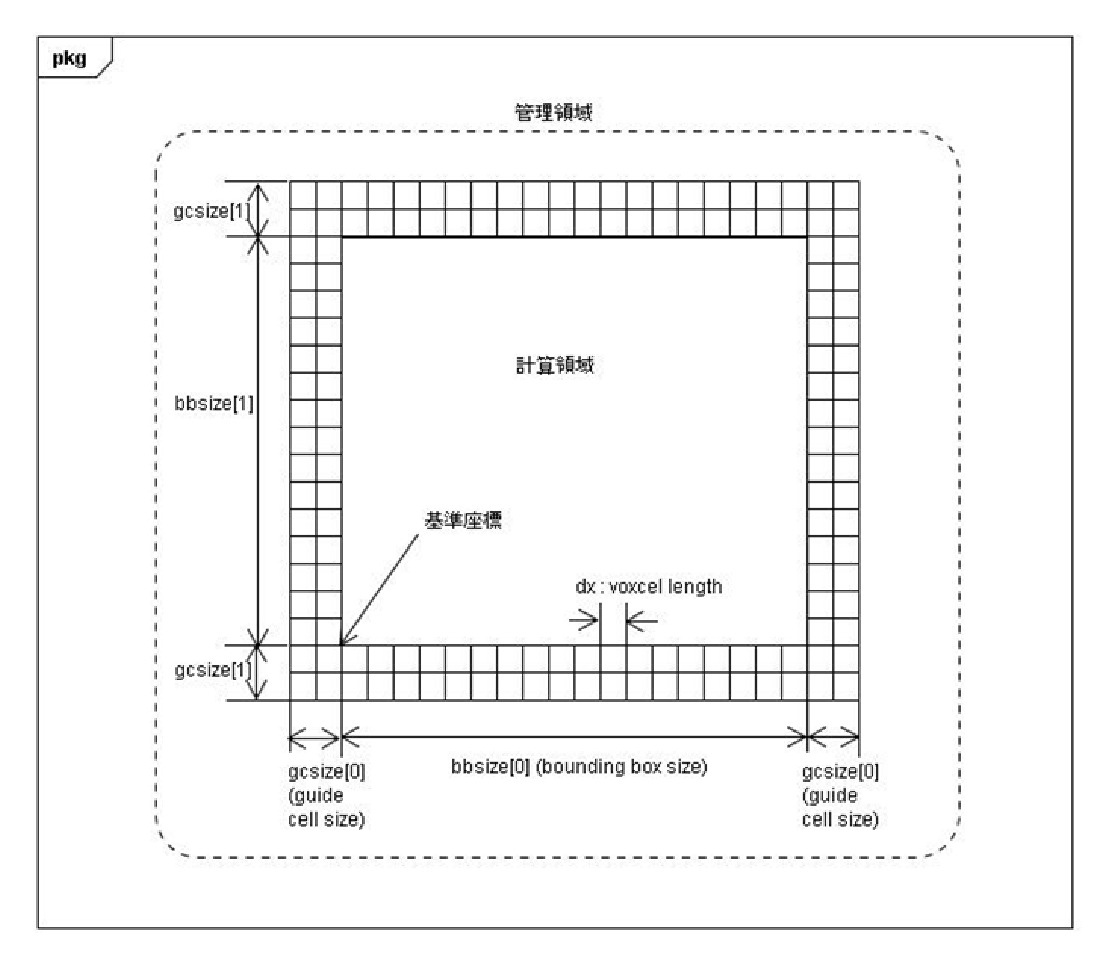
\includegraphics[width=12cm,clip]{clip006.eps}
\caption{計算領域とガイドセル領域の定義}
\label{fig:cal. region}
\end{center}
\end{figure}


\item セルIDの設定\\
V-Xgenで作成したボクセルモデルファイルを,アプリケーションV-Xpp\index{V-Xpp}を用いてセルIDを編集します\footnote{次のバージョンでは,V-Xppの機能をV-Xgenに統合予定です.}.V-Xppを起動し,\verb|File > Open...|を実行してボクセルモデルファイル(*.svx, *.sbx, *.ovx)を選択しロードすると,\textbf{図\ref{fig:V-Xpp voxel}}のようにボクセライズされた形状データが表示されます.\\

 次に,\verb|Volume > Medium List...|を選択し,\textbf{図\ref{fig:V-Xpp Medium list}}に示すセルIDリストを編集します.
ボクセルモデルを\verb|VOI > Select VOI...|や\verb|VOI > Slice Control...|によりボクセルを選択,\verb|VOI > Set Cell ID...|コマンド(\textbf{図\ref{fig:V-Xpp set cell ID}})によりセルIDを選択対象セルに設定します.
セルIDを編集したボクセルモデルは\textbf{図\ref{fig:editted voxel}}のようになるのでファイルに保存します.
ここで,約束事として,\textbf{セルID=0は予約番号でユーザは設定しないこと}に注意してください.\\

また,利用できるIDの設定数に関しては,\hyperlink{tgt:innerboundary}{InnerBoundary}で説明していますが,\textbf{指定できる内部境界条件の数は30個が上限で,かつ指定境界条件数と媒質数の和は63個以下}となる点に注意してください.

\begin{figure}[htbp]
\begin{minipage}{.48\textwidth}
\begin{center}
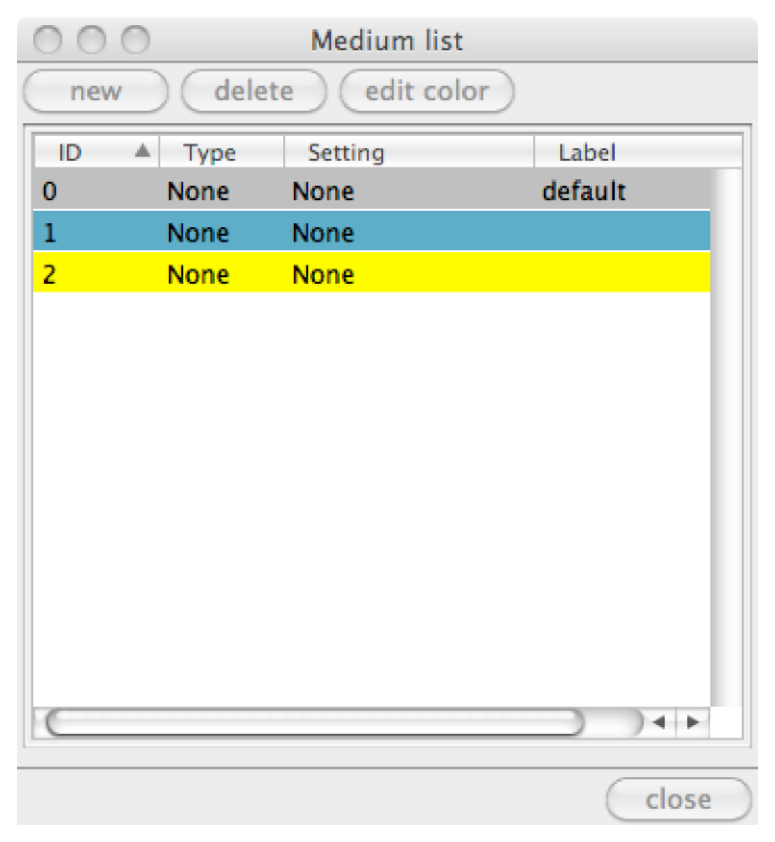
\includegraphics[width=6cm,clip]{VXpp_Mlist.eps}
\end{center}
\caption{セルID編集ダイアログ}
\label{fig:V-Xpp Medium list}
\end{minipage} \hfill
\begin{minipage}{.48\textwidth}
\begin{center}
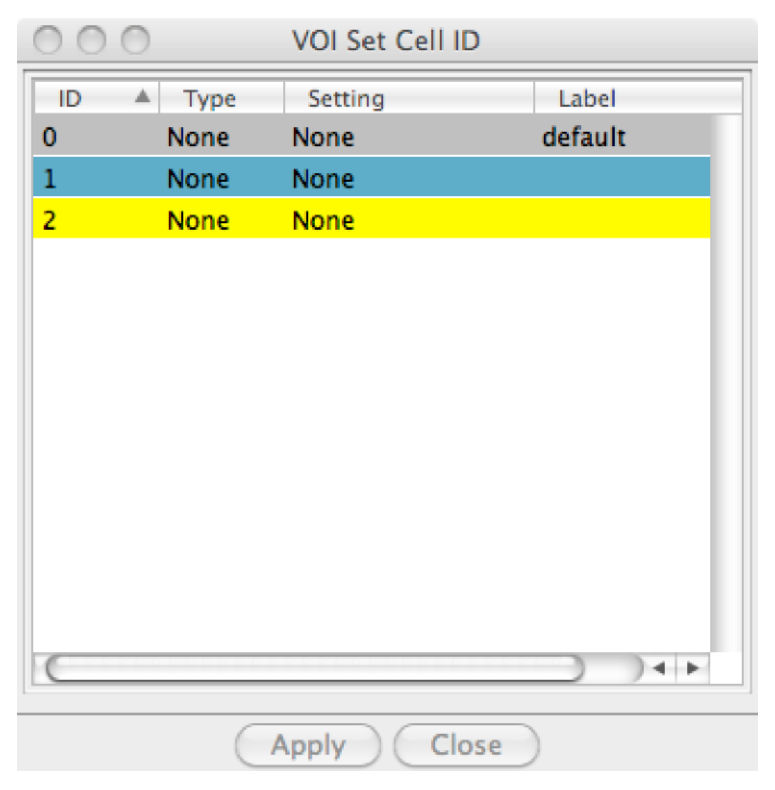
\includegraphics[width=6cm,clip]{VXpp_setID.eps}
\end{center}
\caption{セルID設定ダイアログ}
\label{fig:V-Xpp set cell ID}
\end{minipage}
\end{figure}

\begin{figure}[htdp]
\begin{center}
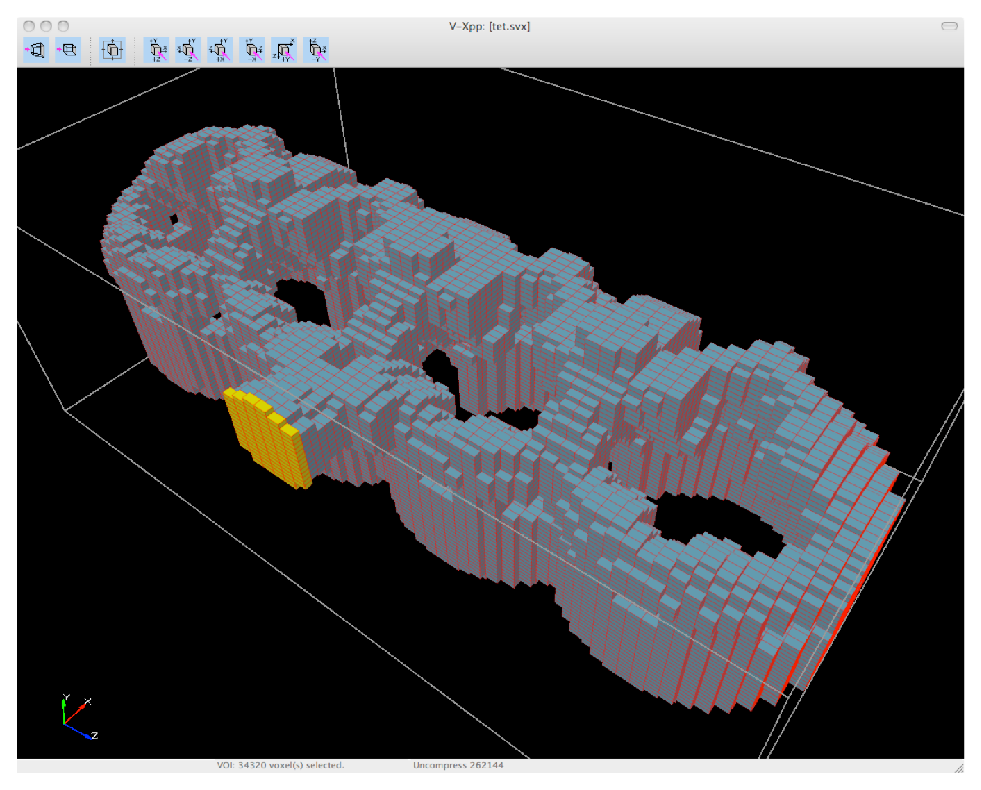
\includegraphics[width=12cm,clip]{VXpp_coloredVoxel.eps}
\caption{V-XppでセルIDを編集したボクセルモデル}
\label{fig:editted voxel}
\end{center}
\end{figure}

\end{enumerate}

\pagebreak


%% 
\section{組み込みモデル}
\hypertarget{tgt:intrinsic model}{組み込みモデル}は,CBCソルバーに組み込み済みの解析モデルです.プログラムに組み込まれた解析モデルを用いることにより,解析モデルを作成しなくても計算ができます.ただし,\textbf{表\ref{tbl:intrinsic problems}}に示すような簡単な形状のモデルに限られます.
各モデルに固有のパラメータは,Parameter $>$ Intrinsic\_Exampleセクションで指定します.

\begin{table}[htdp]
\caption{組み込みモデルクラス}
\begin{center}
\small
\begin{tabular}{lll}\toprule
組み込みモデル名 & 利用クラス & 説明\\ \midrule
Users & IP\_Users & ユーザ問題(解析モデルファイルを指定する場合)\\ \hline
Back\_Step & IP\_STEP & バックステップ流れのモデル\\
Cylinder & IP\_CYLINDER & 角柱と円柱周りの流れのモデル\\
Duct & IP\_Duct & 円形と正方形のダクト流れのモデル\\
Parallel\_Plate\_2D & IP\_PPLT2D & 二次元平行平板のモデル(Poiseuille流れ,Couette流れなど)\\
Performance\_Test & IP\_PMT & 性能測定を行うためのモデル(三次元立方体キャビティフローと同じ問題設定)\\
Polygon & IP\_Polygon & 距離情報スキームを用いる場合に,入力するポリゴンファイル名とDomainInfoの指定だけで計算するモデル\\
Rectangular & IP\_Rect & 計算領域が矩形で,かつ単一媒質の例題のモデル\\
SHC1D & IP\_SHC1D & 一次元の熱伝導問題のモデル\\ 
\bottomrule
\end{tabular}
\end{center}
\label{tbl:intrinsic problems}
\end{table}

%
\subsection{IP\_STEPクラス}
バックステップ流れを計算するクラスです.
\textbf{図\ref{fig:ip_backstep}}と\textbf{表\ref{tbl:ip_backstep}}および\textbf{表\ref{tbl:ip_backstep_ID}}に示すパラメータで計算空間を構成します.
計算領域は,Domain\_Infoで指定するVoxelSize,VoxelPitch,VoxelOriginで決まります.

ドライバー部分については,Ductクラスの設定を参照してください.

\begin{figure}[htdp]
\begin{center}
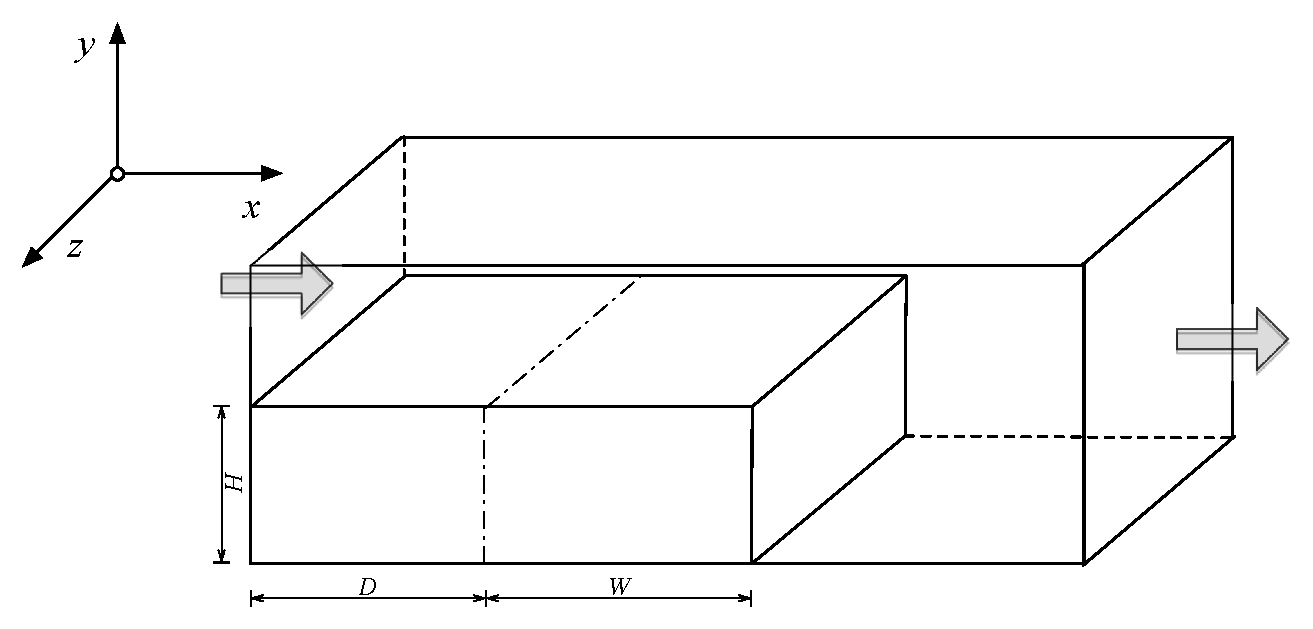
\includegraphics[width=14cm,clip]{Backstep.eps}
\end{center}
\caption{バックステップ流れの計算モデル.}
\label{fig:ip_backstep}
\end{figure}

\begin{table}[htdp]
\small
\caption{バックステップ問題のパラメータ.}
\begin{center}
\begin{tabular}{ll}\toprule
記号 & パラメータ\\ \midrule
Mode & 2D $|$ 3D\\ \hline
Width ($W$) & ステップの$x$方向の幅\\
Height ($H$) & ステップの$y$方向の高さ\\
Driver ($D$) & ドライバー部分の長さ($>0.0$でドライバあり,=0.0の場合ドライバーなし)\\
\bottomrule
\end{tabular}
\end{center}
\label{tbl:ip_backstep}
\end{table}

\begin{table}[htdp]
\small
\caption{バックステップ問題のID番号.}
\begin{center}
\begin{tabular}{ll}\toprule
ID & 属性\\ \midrule
1 & 流体\\
2 & 固体\\
3 & ドライバ部分の流体\\
4 & ドライバ流出面(流体)\\
\bottomrule
\end{tabular}
\end{center}
\label{tbl:ip_backstep_ID}
\end{table}

境界条件として,X-方向に流入,またはドライバ境界,X+方向は流出条件,Y-方向は壁面,Y+方向は壁面またはスリップ条件,Z$\pm$方向は壁面か周期境界を与えて計算します.二次元の問題を解く場合には,Mode=2Dを指定,VoxelSizeはkmax=3として,Z方向は周期境界条件を与えてください.

%
\subsection{IP\_CYLINDERクラス}
二次元と三次元の円柱・角柱まわりの流れを計算するクラスです.
\textbf{図\ref{fig:ip_cylinder}}と\textbf{表\ref{tbl:ip_cylinder}}に示すパラメータで計算空間を構成します.
断面形状は,円柱と角柱をShapeで指定します.それぞれの断面形状で指定するパラメータが異なります.
柱は$xy$平面の$z-$方向に接しています.これを基準に長さのパラメータを指定してください.

二次元の問題を解く場合には,Mode=2Dを指定,VoxelSizeはkmax=3としてください.この場合,パラメータ$W$は無視されます.

\begin{figure}[htdp]
\begin{center}
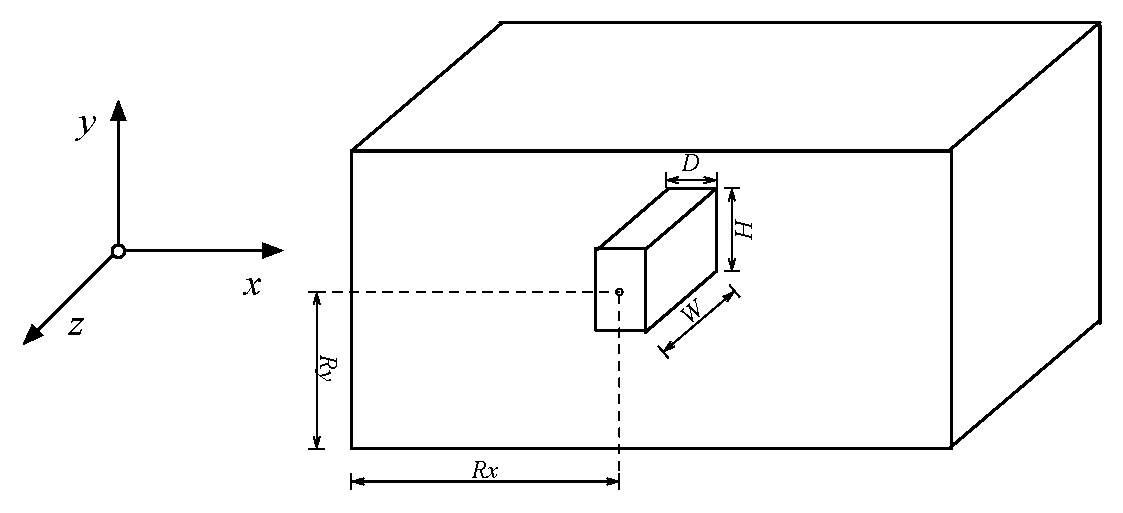
\includegraphics[width=14cm,clip]{Cylinder.eps}
\end{center}
\caption{円柱・角柱モデルの計算空間.}
\label{fig:ip_cylinder}
\end{figure}

\begin{table}[htdp]
\small
\caption{柱状物体の指定パラメータ}
\begin{center}
\begin{tabular}{ll}\toprule
記号 & パラメータ\\ \midrule
Mode & 2D $|$ 3D\\ 
Shape & Rectangular $|$ Circular\\ \hline
$D$ & 角柱を指定時の角柱の幅\\
$H$ & 角柱を指定時の角柱の高さ\\
$R$ & 円柱を指定時の半径\\
$W$ & 柱の$z$軸方向の長さ\\
$R_x$ & 柱の中心位置と$x$方向領域境界からの距離\\
$R_y$ & 柱の中心位置と$y$方向領域境界からの距離\\
\bottomrule
\end{tabular}
\end{center}
\label{tbl:ip_cylinder}
\end{table}

%
\subsection{IP\_Ductクラス}
\textbf{図\ref{fig:ip_duct}}のような円形と矩形のダクト流れを計算するモデルで,周期境界条件を用います.
流入面には,流れを発達させる機能をもつドライバー部分を指定することができます.

断面形状は,正方形または円形をShapeで指定し,
流入部の方向をDirectionで指定します.
ドライバー部は,Directionで指定した方向にドライバ部分が配置されます.
ドライバー部分を指定する場合には,Driverにその長さ$D$を指定してください.
$D=0.0$の場合には,ドライバー無しの指定になります.

\begin{figure}[htdp]
\begin{center}
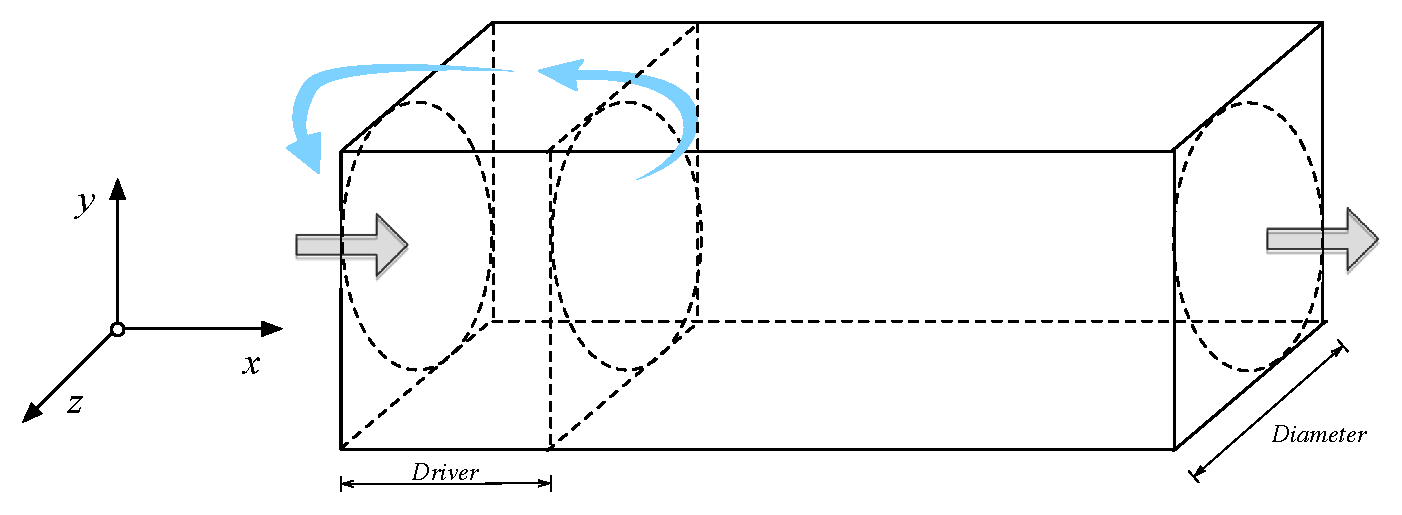
\includegraphics[width=16cm,clip]{Duct.eps}
\end{center}
\caption{ダクトの計算空間.$X-$方向にドライバ部を設置した場合.}
\label{fig:ip_duct}
\end{figure}

\begin{table}[htdp]
\small
\caption{ダクトの指定パラメータ}
\begin{center}
\begin{tabular}{ll}\toprule
記号 & パラメータ\\ \midrule
Shape & Rectangular $|$ Circular\\ \hline
Diameter & 正方形または円の直径\\
Direction & 周期境界と流入の方向(X\_minus, X\_plus, Y\_minus, Y\_plus, Z\_minus, Z\_plus)\\
Driver & ドライバー部分の長さ($>0.0$でドライバあり,=0.0の場合ドライバーなし)\\
\bottomrule
\end{tabular}
\end{center}
\label{tbl:ip_duct}
\end{table}


%
\subsection{IP\_PMTクラス}
CBCソルバークラスの基本的性能を測定するための例題クラスです.
三次元立方体の空間内のキャビティフローを解きます.
性能測定モードとなり,圧力反復の収束判定は行わず,反復回数は固定となります.
また,初期化時のファイル出力が抑制されます.

%
\subsection{IP\_PPLT2Dクラス}
二次元の平行平板間の流れを計算するためのクラスです.
\textbf{図\ref{fig:pplate2d}}のように辺長比が2:1の二次元空間を表現します.
z方向には3セルを設けており,単純な周期境界条件を用いて二次元を近似しています.
したがって,VoxelSizeでは\lq\lq kmax=3 \rq\rq を指定し,分割数imaxとjmaxの比は2:1となるように指定します.
空間格子幅は,x方向とy方向で同じ(直交等間隔)としています.

計算領域内部は単一媒質(セルID=1)が設定されています.
この例題は,パラメータ指定\lq\lq Unit\_of\_input\_parameter\rq\rq に無次元を指定します.

\begin{figure}[htdp]
\begin{center}
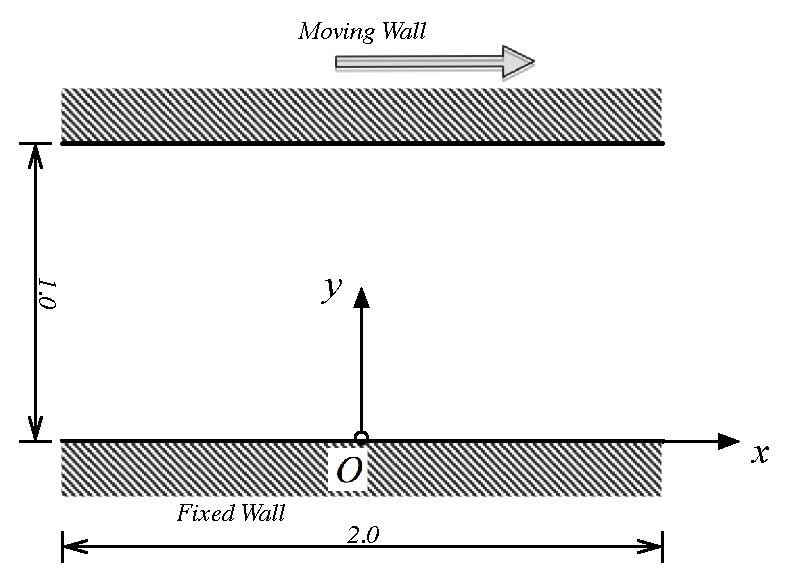
\includegraphics[width=8cm,clip]{PPLT2D.eps}
\end{center}
\caption{二次元平行平板間の計算空間.}
\label{fig:pplate2d}
\end{figure}


%
\subsection{IP\_Rectクラス}
IP\_Rectクラスは三次元の矩形の計算領域を表現するクラスで,計算領域内部は単一媒質(セルID=1)が設定されています.
計算領域は,次のようにDomainInfoタグで指定します.ここでは,各方向の分割数を64に指定し,基点座標が$(-0.5, -0.5, -0.5)$,ボクセルピッチを$pch=1.5625\times10^{-2}$に指定しています.
VoxelSizeとVoxelPitchのパラメータは,\textbf{図\ref{fig:rect intrinsic class}}に示すように,格子幅$pch$と分割数$imax$がそれぞれ対応しています.


{\small
\begin{program}
<DomainInfo>
  <VoxelOrigin ox="-0.5" oy="-0.5" oz="-0.5"/>
  <VoxelSize ix="64" jx="64" kx="64"/>
  <VoxelPitch dx="1.5625e-02" dy="1.5625e-02" dz="1.5625e-02"/>
</DomainInfo>
\end{program}
}


\begin{figure}[htdp]
\begin{center}
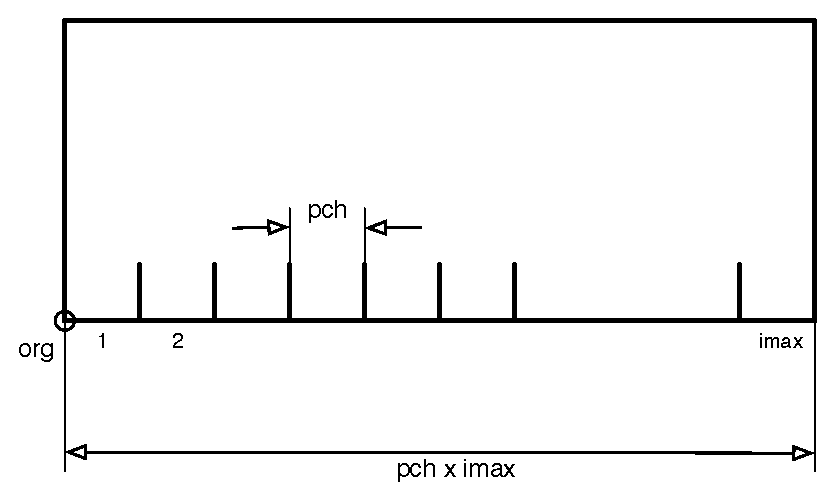
\includegraphics[width=9cm,clip]{rect.eps}
\caption{Rectangularクラスのパラメータ設定}
\label{fig:rect intrinsic class}
\end{center}
\end{figure}


\begin{table}[htdp]
\caption{Intrinsic\_Exampleタグで設定可能なパラメータ}
\begin{center}
\small
\begin{tabular}{lll}\toprule
指定パラメータ & 指定値 & 意味\\ \midrule
Check\_Even & Yes $|$ No & 分割数が偶数であるかどうかをチェックする\\
\bottomrule
\end{tabular}
\end{center}
\label{tbl:rect parameter}
\end{table}

\textbf{表\ref{tbl:rect parameter}}のパラメータは,Parameter $>$ Intrinsic\_Exampleセクションで指定します.

{ \small
\begin{program}
<Elem name="Intrinsic_Example">
  <Param dtype="STRING" name="Check_Even" value="Yes"/>
</Elem>
\end{program}
}

上記のパラメータ設定では,分割数の偶数チェックを行います.

%
\subsection{IP\_Polygonクラス}
XMLファイルで,\lq\lq Steer > Solver\_Property > Shape\_Approximation\rq\rq でDistance\_Infoを指定すると,距離情報を用いたスキームで計算します.
この\hypertarget{tgt:polygon_class}{IP\_Polygonクラス}は,入力するポリゴンファイルと,DomainInfoで指定する計算領域情報のみで計算を行うモデルテンプレートです.ポリゴンファイル名は,\lq\lq Steer > Polygon\_File\rq\rq で指定します.

%
\subsection{IP\_SHC1Dクラス}
\textbf{図\ref{fig:HC1D}}に示すような片持ちはりの熱伝導問題を一次元の定常熱伝導問題として解くためのクラスです.
この問題には厳密解があり,厳密解と計算結果を比較することにより予測精度の確認ができます.

\begin{figure}[htdp]
\begin{center}
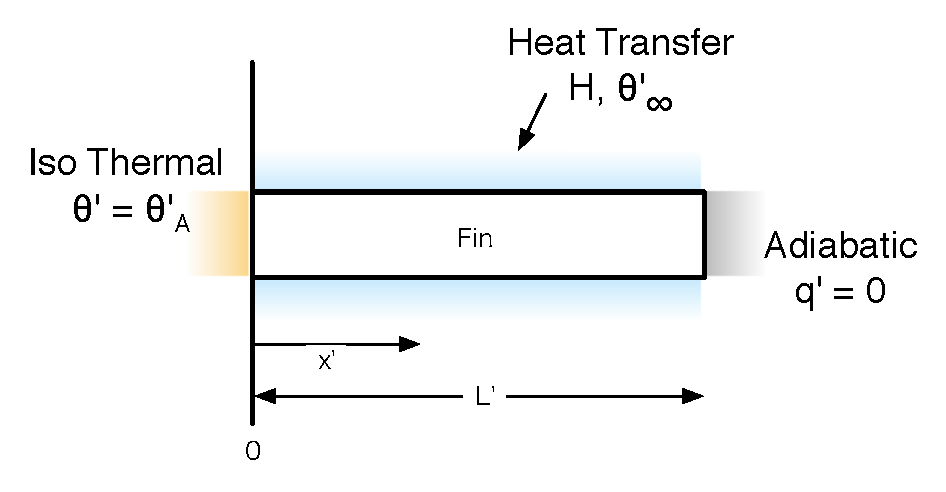
\includegraphics[width=9cm,clip]{1DHC.eps}
\end{center}
\caption{一次元定常熱伝導問題の模式図}
\label{fig:HC1D}
\end{figure}


計算領域は\textbf{図\ref{fig:HC model}}に示すようにx軸方向に放熱フィンをとり,y,z方向には5つだけセルを設けます.
領域の設定パラメータとして,x方向の分割数をimaxにより与えます.
放熱フィンを5分割したい場合には,imax=7を設定します.
その他の方向は$\mathrm{jmax=kmax=5}$で固定です.

例題と解析結果の詳細については,例題集をご覧ください.

\begin{figure}[htdp]
\begin{minipage}{0.47\hsize}
\begin{center}
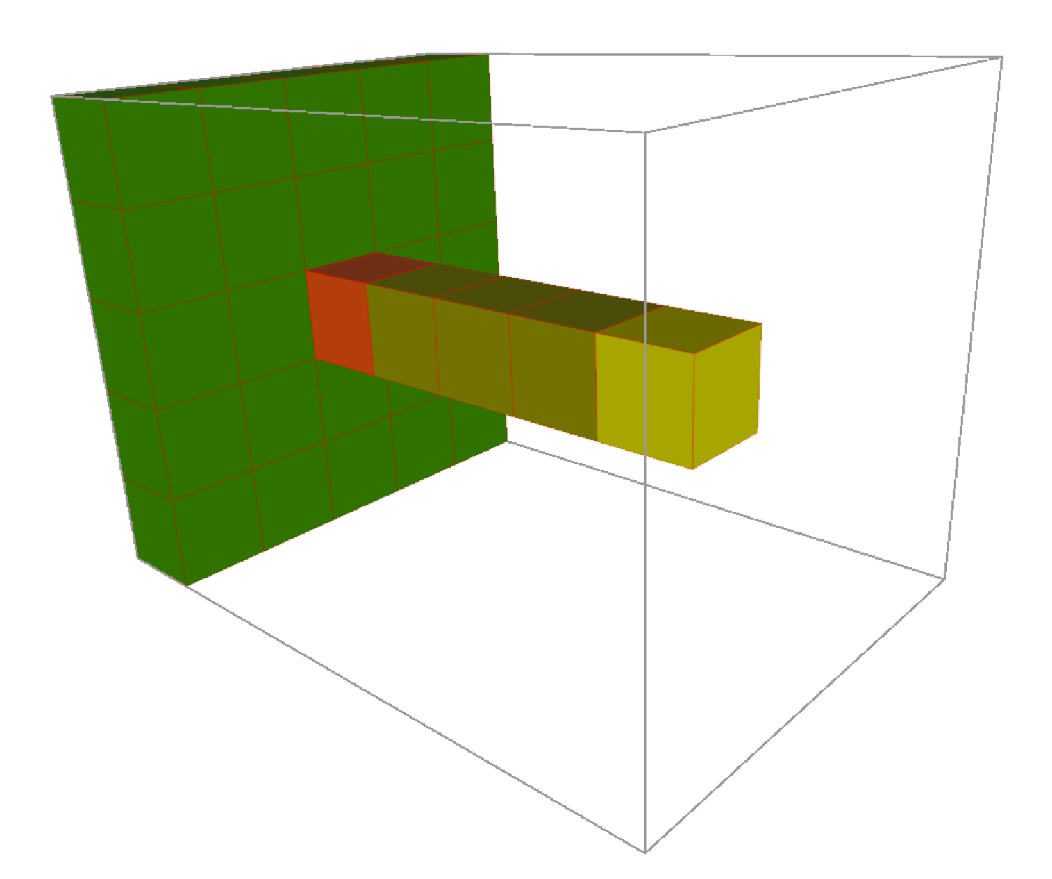
\includegraphics[height=5cm,clip]{model_iso.eps}
\end{center}
\end{minipage}
\begin{minipage}{0.47\hsize}
\begin{center}
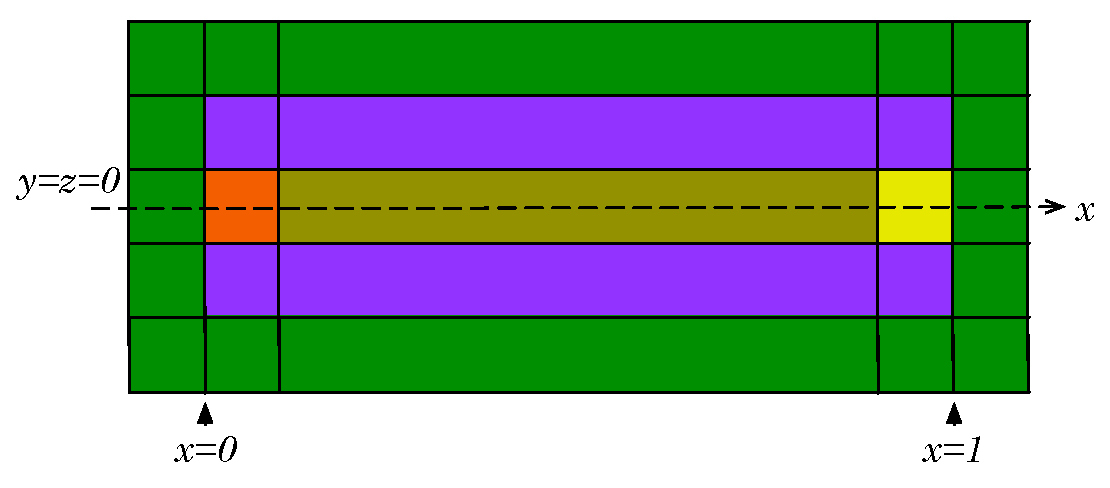
\includegraphics[height=3.5cm,clip]{dimension.eps}
\end{center}
\end{minipage}
\caption{一次元熱伝導問題を計算するための片持ち梁の三次元モデルとセルID (分割数が$7\times5\times5$の場合)}
\label{fig:HC model}
\end{figure}


\pagebreak
% 
\section{例題}
ソースファイルのExampleディレクトリに含まれる\hypertarget{tgt:samples}{例題}について説明します.
提供される例題は,組み込みモデルや簡単なボクセルモデルを同梱した例題群で,
基本的な流れやソルバーの検証のために用意されています.


\begin{table}[htdp]
\caption{組み込み例題}
\begin{center}
\small
\begin{tabular}{lll} \toprule
Example & Class & Comment\\ \midrule
Cavity flow 3D (Cube) & IP\_Rect & 三次元立方体キャビティフロー\\
LDC112  & IP\_Rect & Guermondの実験に対応する辺長が1:1:2のキャビティフロー\\ 
Duct 3D & IP\_Duct3D & ダクト流れ\\ 
PMT & IP\_PMT & 性能測定を行うための例題(三次元立方体キャビティフローの例題と同じ)\\
\bottomrule
\end{tabular}
\end{center}
\label{tbl:example at glance}
\end{table}

\begin{table}[htdp]
\caption{サンプル例題}
\begin{center}
\small
\begin{tabular}{lll} \toprule
Example & Comment\\ \midrule
Dragon & Asian Dragon周りの流れ\\
Heated Plate & 流体中の平板からの放熱\\
SHC1D & 熱伝導計算の解析解との比較\\ \bottomrule
\end{tabular}
\end{center}
\label{tbl:exercise}
\end{table}





%%%
\chapter{制御と物理パラメータ}
\label{chpt:param}
\begin{abstract}
V-Sphereシステム上の入力パラメータは,データベースなどでの再利用性を考慮し,XML(eXtensible Markup Language)形式で記述します.XMLはタグ構造のデータ記述言語で,階層的な要素の記述が可能なマークアップ言語です.このXMLデータをV-Sphere内部でツリー状のオブジェクトとして構文解析および操作します.
本章では,CBCソルバークラスの制御と物理パラメータ(これをコンフィギュレーションファイル\index{ふぁいる@ファイル!こんふぃぎゅれーしょん@コンフィギュレーション---}と呼びます)について説明します.境界条件の詳細については,CBCソルバークラス説明書をご覧ください.
\end{abstract}
%
\graphicspath{{./fig_Param/}}

%
\section{XMLコンフィギュレーションファイル}
%
\subsection{XML記述}
XML\index{XML}文書の先頭行は,\verb|<?xml version="1.0"?>|で始まり,このXML文書はXML 1.0 の規格を満たす文書であることを示しています.
XMLの要素は,\verb|<>..</>|で囲まれた対になったタグ\index{えっくすえむえる@XML!たぐ@---のタグ}で表現されます.ここでは,タグで囲まれている部分をセクション\index{えっくすえむえる@XML!せくしょん@---のセクション}と呼びます.
{
\small 
\begin{program}
<keyword>
	...
</keyword>
\end{program}
}


\noindent 一行内で終わるような短い要素の場合は,次のようにスラッシュで終わる形式で記述できます.
\vspace{2mm}

{
\small 
\begin{program}
<Param name="Output_Mode" dtype="STRING" value="forced" />
\end{program}
}

\noindent 要素を無効にする場合には,前後を\verb|<!-- *** -->|のように!と2連のマイナス記号で囲みます.
\vspace{2mm}

{
\small 
\begin{program}
<!--StartCondition type="Restart"/-->
\end{program}
}


%
\subsection{コンフィギュレーションファイルの構造}
コンフィギュレーションファイルは,ソルバークラスの入力ファイルとしての役割を果たします.
コンフィギュレーションファイルの中にあるSphereConfigタグ\index{SphereConfig}は,そこに記述された内容がV-Sphereのコンフィギュレーションであることを示します.クォーテーション(“”)で囲まれた文字列は,大文字でも小文字でもかまいません.

{
\small 
\begin{program}
<SphereConfig SolverType="CBC" >
	...
</SphereConfig>
\end{program}
}

\noindent \verb|SolverType="CBC"|\index{SolverType}は,V-Sphereが実行時にインスタンスするソルバクラスのキーワードを示します.このキーワードが,V-Sphereに登録されていない場合はエラーとなります.
SphereConfig内には,\textbf{表\ref{tbl:SphereConfig_tag}}に示すタグが記述されています.
コンフィギュレーションファイルの名称は任意で,このうち媒質情報と境界条件の内容の記述はSphereConfigタグ内に直接記述してもよいし,指定したファイルに記述しても構いません.両方存在する場合には,SphereConfigタグ内の記述が優先されます.\\

\begin{table}[htdp]
\caption{SphereConfig内のセクション}
\begin{center}
\small
\begin{tabular}{ll} \toprule
タグ & パラメータ\\ \midrule
DomainInfo & 計算領域\\
Steer & ソルバー制御\\
Parameter & 計算条件\\
BC\_Table & 境界条件\\
Medium\_Table & 媒質情報\\ \bottomrule
\end{tabular}
\end{center}
\label{tbl:SphereConfig_tag}
\end{table}


V-Sphereには,SPHERE定義要素\index{sphereていぎようそ@SPHERE定義要素}とソルバ定義要素\index{そるばていぎようそ@ソルバ定義要素}の2種類があります.SPHERE定義要素は,V-Sphereフレームワーク側で規定されたタグで,ソルバ定義要素はElem, Param要素で構成される汎用記述要素です.ソルバ定義要素のdtypeはデータの型(STRING, INT, REAL)を表し,valueは指定された型に対応した値をとります.

\pagebreak
%
\section{パラメータの詳細}
%
\subsection{DomainInfoセクション}
%
\subsubsection{DomainInfo}

\hypertarget{tgt:domaininfo}{DomainInfo}では,ボクセルモデル情報と外部ファイル情報を指定します.

\begin{indentation}{3zw}{0zw}

{\small
\begin{program}
<DomainInfo>
  <VoxelSize   ix="64" jx="64" kx="64" />
  <VoxelOrigin ox="0.0" oy="0.0" oz="0.0" />
  <VoxelPitch  dx="0.0" dy="0.0" dz="0.0" />
  <Param name="MDMTBL" dtype="STRING" value="xml/medium.xml" />
  <Param name="BCTBL"  dtype="STRING" value="xml/boundary.xml" />
  <Param name="MBXTBL" dtype="STRING" value="xml/multibox.xml">
</DomainInfo>
\end{program}
}

ボクセルモデル情報については,\textbf{表\ref{tbl:voxel info}}に示す計算領域に関するパラメータを指定します.この計算領域情報は,\hyperlink{tgt:example}{ユーザ問題と組み込み例題}とで指定内容が異なります.
組み込み例題の場合には,例題に応じて情報を指定します.
一方,ユーザ問題では,入力となる解析モデルファイルから,ボクセルのサイズやピッチなどのパラメータを取得します.

外部ファイル情報については,\textbf{表\ref{tbl:file info}}に示すように,媒質情報ファイル,境界条件情報ファイル,多連結領域の分割情報について,外部ファイルとして記述する場合にファイルのパスを指定できます.

\begin{table}[htdp]
\caption{DomainInfoセクションにおける計算領域パラメータの指定}
\begin{center}
\small
\begin{tabular}{ll} \toprule
タグ & 指定内容\\ \midrule
VoxelSize & 計算空間の各軸方向の分割数\\
VoxelOrigin & 計算空間における座標値の最小値\\
VoxelPitch & 各軸方向の分割幅\\
VoxelWidth & 計算領域の大きさ\\ \bottomrule
\end{tabular}
\end{center}
\label{tbl:voxel info}
\end{table}

\begin{table}[htdp]
\caption{外部ファイル指定}
\begin{center}
\small
\begin{tabular}{ll} \toprule
タグ & 説明\\ \midrule
MDMTBL & 媒質情報を記述したコンフィギュレーションファイルの指定\\
BCTBL  & 境界条件を記述したコンフィギュレーションファイルの指定\\
MBXTBL & 多連結領域分割計算時の分割情報ファイルの指定\\ \bottomrule
\end{tabular}
\end{center}
\label{tbl:file info}
\end{table}

\end{indentation}

\pagebreak
%
\subsection{Steerセクション}
\label{sec:steer}
Steerセクションでは,CBCソルバークラスの実行制御パラメータ\index{じっこうせいぎょぱらめーた@実行制御パラメータ}を記述します.\\

%
\subsubsection{Algorithm}

時間積分と\hypertarget{tgt:algorithm}{解法アルゴリズム}の組み合わせを選択するパラメータです.

\begin{indentation}{3zw}{0zw}

{\small
\begin{program}
<Elem name="Algorithm">
  <Param name="Flow"   dtype="STRING" value="FS_C_EE_D_EE"/>
  <Param name="Heat"   dtype="STRING" value="C_EE_D_EE"/>
</Elem>
\end{program}
}

\textbf{表\ref{tbl:alg_flow}}に時間進行法と分離解法の種類の組み合わせを示します.Flowパラメータでは流動の支配方程式の時間積分法と解法アルゴリズムの組み合わせを指定します.
%時間二次精度以上を選択した場合には,\verb|Convection_Term|\ref{sec:p_convection}では二次以上の空間スキームしか選択できません.\\

\begin{table}[htdp]
\caption{流動解析のアルゴリズム選択パラメータ指定}
\begin{center}
\small
\begin{tabular}{ll} \toprule
キーワード & 時間積分法と解法の組み合わせ\\ \midrule
FS\_C\_EE\_D\_EE & Fractional Step法 + 時間一次精度Euler陽解法(対流項と拡散項)\\ \bottomrule
%FS\_C\_RK\_D\_CN & FS法 + 時間二次精度 Runge-Kutta陽解法(対流項)+ Crank-Nicholson陰解法(拡散項)\\
%FS\_C\_RK\_D\_ME & FS法 + 時間二次精度 Runge-Kutta陽解法(対流項)+ Modified-Euler陽解法(拡散項)\\
%FS\_C\_AB\_D\_AB & FS法 + 時間二次精度 Adams-Bashforth陽解法(対流項と拡散項)\\ \bottomrule
\end{tabular}
\end{center}
\label{tbl:alg_flow}
\end{table}

温度解析の場合には,Heatパラメータで温度輸送方程式の時間進行法と解法アルゴリズムの組み合わせを示します.指定できるパラメータは\textbf{表\ref{tbl:alg_heat}}に示します.\\

\begin{table}[htdp]
\caption{温度解析のアルゴリズム選択パラメータ指定}
\begin{center}
\small
\begin{tabular}{ll} \toprule
キーワード & 時間積分法と解法の組み合わせ\\ \midrule
C\_EE\_D\_EE & 時間一次精度 Euler陽解法(対流項と拡散項)\\
C\_EE\_D\_EI & 時間一次精度 Euler陽解法(対流項)+ Euler陰解法(拡散項)\\ \bottomrule
%C\_AB\_D\_AB & 時間二次精度 Adams-Bashforth陽解法(対流項と拡散項)\\ \bottomrule
\end{tabular}
\end{center}
\label{tbl:alg_heat}
\end{table}
\end{indentation}



%%%
\pagebreak
\subsubsection{Average\_Option}

\hypertarget{tgt:average_option}{時間平均操作}に関するパラメータを指定します.

\begin{indentation}{3zw}{0zw}

{\small
\begin{program}
<Elem name="Average_Option">
  <Param name="Operation"    dtype="STRING" value="On" />
  <Param name="Start_Type"   dtype="string" value="time" />
  <Param name="Start"        dtype="REAL"   value="500.0" />
</Elem>
\end{program}
}

\textbf{表\ref{tbl:averaging}}に物理量の時間平均操作\index{じかんへいきんそうさ@時間平均操作}を指定するパラメータを示します.
CBCソルバークラスは非定常解析を行いますので,流れの挙動が準定常状態になったところで時間平均操作を開始し,十分な長さで時間平均操作が行われた速度場や温度場を定常解\index{ていじょうかい@定常解}とみなします.
時間平均操作の開始時刻はStartで指定し,この開始時刻以降,毎ステップごとに時間平均操作を行います.
平均操作の開始時刻は,Start\_Typeで指定する方法に依存し,
Timeを指定した場合にはUnit\_of\_Input\_Parameterの次元に従います.
つまり,\hyperlink{tgt:unit}{value}=\lq\lq DIMENSIONAL\rq\rq の場合には有次元時刻で時間平均操作の開始時刻を指定することになります.

時間平均場の出力タイミングは,\hyperlink{tgt:fileio}{File\_IO}のAveraged\_Intervalで指定します.


\begin{table}[htdp]
\caption{Average\_Optionのパラメータ}
\begin{center}
\small
\begin{tabular}{ll} \toprule
キーワード & 指定パラメータ\\ \midrule
Operation & On $|$ Off\\
Start\_Type & 開始時刻の指定 (Step $|$ Time)\\
Start & 時間平均操作の開始時刻\\ \bottomrule
\end{tabular}
\end{center}
\label{tbl:averaging}
\end{table}

\end{indentation}



%%%
\pagebreak
\subsubsection{Check\_Parameter}

ボクセルモデルと入力パラメータの\hypertarget{tgt:check_parameter}{整合性のチェック}を行い,初期設定後にソルバーを停止します.

\begin{indentation}{3zw}{0zw}

{\small
\begin{program}
<Param name="Check_Parameter" dtype="STRING" value="On"/>
\end{program}
}

Check\_Parameter=\lq\lq On\rq\rq でチェックが有効な場合,V-Sphereを起動してパラメータを読み込み,前処理が終了した段階でCBCソルバーを強制終了します.
このとき,初期設定パラメータの内容がconditions.txtに書き出されているので,パラメータのチェックができます.
また,初期条件を与えたフィールドファイルが出力されるので,初期条件のチェックが可能です.

\end{indentation}



%%%
\pagebreak
\subsubsection{Convection\_Term}

\hypertarget{tgt:convection_term}{対流項のスキーム}に関するパラメータを指定します.

\begin{indentation}{3zw}{0zw}

{\small
\begin{program}
<Elem name="Convection_Term">
  <Param name="Scheme"   dtype="STRING" value="O3_MUSCL" />
  <Param name="Limiter"  dtype="STRING" value="minmod" />
</Elem>
\end{program}
}

SchemeとLimiterのパラメータを\textbf{表\ref{tbl:scheme limiter}}に示します.Limiterは制限関数\index{せいげんかんすう@制限関数}の種類を示し,Schemeが\verb|O3_MUSCL|の場合のみ有効となります.
非圧縮流れのように物理量の変化が連続的な場合には不要の場合もあります.
ファイル出力時のオプションでガイドセル出力\hyperlink{tgt:fileio}{Guide\_Out}=\lq\lq with\rq\rq を指定している場合には,対流項スキームによってステンシル\index{ステンシル}が変化するので,ガイドセル\index{ガイドセル}の値も異なります.

\begin{table}[htdp]
\small
\caption{SchemeとLimiterのパラメータ}
\begin{minipage}{.6\textwidth}
\begin{center}
\begin{tabular}{llc} \toprule
Scheme & 指定スキーム & 出力ガイドセルサイズ\\ \midrule
O1\_Upwind & 一次精度風上スキーム & 1\\
O2\_Central & 二次精度中心スキーム & 1\\
O3\_MUSCL & 三次精度MUSCLスキーム & 2\\ \bottomrule
\end{tabular}
\end{center}
\end{minipage} \hfill
\begin{minipage}{.38\textwidth}
\begin{center}
\begin{tabular}{ll} \toprule
Limiter & 制限関数\\ \midrule
Minmod & minmod型\\
No\_Limiter & | \\ \bottomrule
\end{tabular}
\end{center}
\end{minipage}
\label{tbl:scheme limiter}
\end{table}

\end{indentation}



%%%
\pagebreak
\subsubsection{Derived\_Variable}

\hypertarget{tgt:derived_variable}{派生変数}(基本変数から計算される変数)の生成を指定します.

\begin{indentation}{3zw}{0zw}

{\small
\begin{program}
<Elem name="Derived_Variable">
  <Param name="Total_Pressure"       dtype="STRING" value="off" />
  <Param name="2nd_Invariant_of_VGT" dtype="STRING" value="on" />
  <Param name="Helicity"             dtype="STRING" value="on" />
  <Param name="Vorticity"            dtype="STRING" value="on" />
</Elem>
\end{program}
}

\textbf{表\ref{tbl:derived vars}}に示す各変数は,on/offのスイッチ指定により有効・無効になり,\hyperlink{tgt:fileio}{File\_IO}セクションのInstant\_Intervalで指定するタイミングでファイルに出力されます.value=\lq\lq off\rq\rq の場合には,OutFileタグの記述は無効となります.OutputDataセクションのIntervalでは設定しません.

\begin{table}[htdp]
\caption{派生変数の指定}
\begin{center}
\small
\begin{tabular}{ll}\toprule
タグ & 生成する派生変数\\ \midrule
Total\_Pressure & 全圧\\
Vorticity & 渦度ベクトル\\
Helicity & ヘリシティ\\
2nd\_Invariant\_of\_VGT & 速度勾配テンソルの第二不変量\\ \bottomrule
\end{tabular}
\end{center}
\label{tbl:derived vars}
\end{table}

%
\paragraph{全圧(総圧)}
全圧の計算を指定した場合には,同時に\hyperlink{tgt:output_data}{OutputData}セクションに出力ファイル名を次のように記述します.
attrタグにはTotalPressureを指定し,basenameには任意のプリフィックスを記述します\footnote{ここで指定するInterval属性は無効で,\hyperlink{tgt:interval}{Interval}セクションでの指定に従います.}.

{\small
\begin{program}
<OutFile attr="TotalPressure" Interval="1" format="SPH" basename="tp" />
\end{program}
}

全圧は次式で定義され,単位体積あたりのエネルギーを表します.

\begin{equation}
\frac{1}{2} {u^{\prime}}^{2} + \frac{P^{\prime}}{\rho^{\prime}} \qquad [Pa] \sim [J/m^3]
\label{eq:total pressure}
\end{equation}

非圧縮の場合には,

\begin{equation}
{P_{T}}^{\prime} \,=\, \frac{1}{2} \rho^{\prime} {u^{\prime}}^{2} + P^{\prime} \qquad [J/m^3]
\label{eq:total pressure icmp}
\end{equation}

\textbf{式(\ref{eq:total pressure icmp})}は無次元化すると,以下のようになります.

\begin{equation}
P_{T} \,=\, \frac{{P_{T}}^{\prime}}{\rho_{\mathit{0}}^{\prime} {u_{\mathit{0}}^{\prime}}^{2}}
\label{eq:total pressure icmp ND}
\end{equation}

%
\paragraph{渦度ベクトル}
渦度の計算を指定した場合には,同時に\hyperlink{tgt:output_data}{OutputData}セクションに出力ファイルを次のように記述します.
attrタグにはVorticityを指定し,basenameには任意のプリフィックスを記述します.

{\small
\begin{program}
<OutFile attr="Vorticity" Interval="1" format="SPH" basename="vrt" />
\end{program}
}

%
\paragraph{ヘリシティ}
ヘリシティは速度ベクトル$\overrightarrow{u}$と渦度ベクトル$\overrightarrow{\omega}$の内積として定義される量で次式により表せます.OutFileタグの記述は上記と同様です.

\begin{equation}
H \,=\, \overrightarrow{u} \cdot \overrightarrow{\omega}
\label{eq:helicity}
\end{equation}

{\small
\begin{program}
<OutFile attr="Helicity" Interval="1" format="SPH" basename="hlcty" />
\end{program}
}

%
\paragraph{速度勾配テンソルの第二不変量}
渦構造を可視化するのに利用され,
符号により単純剪断乱流の中の層状渦と管状渦を区別することができます\cite{tanaka:93:PF}.OutFileタグの記述は上記と同様です.
{\small
\begin{program}
<OutFile attr="2ndInvrntVGT" Interval="1" format="SPH" basename="i2vgt" />
\end{program}
}

\end{indentation}



%%%
\pagebreak
\subsubsection{Example}

\hypertarget{tgt:example}{解くべき問題}を指定します.

\begin{indentation}{3zw}{0zw}

{\small
\begin{program}
<Param name="Example" dtype="STRING" value="Users"/>
\end{program}
}

\textbf{表\ref{tbl:intrinsic_example}}にCBCソルバークラスで提供される組み込み例題\index{くみこみれいだい@組み込み例題}の一覧を示します.
表の中で,Usersはユーザーが準備した解析モデルを用いることを指定します.
組み込み例題で固有のパラメータ設定がある場合についてはParameter$\to$\hyperlink{tgt:intrinsic_example}{Intrinsic\_Example}をご覧ください.

また,具体的な例題の事例については,例題集をご覧ください.

\begin{table}[htdp]
\caption{Exampleのパラメータ指定}
\begin{center}
\small
\begin{tabular}{ll} \toprule
キーワード & 解く問題\\ \midrule
Cavity3D & 立方体キャビティ\\
Duct3D & 直方体と円形断面のダクト\\
LDC112 & 辺長比1:1:2の三次元キャビティ\\
Performance\_Test & 性能評価\\
SHC1D & 固体熱伝導\\
Users & ユーザの指定モデル\\ \bottomrule
\end{tabular}
\end{center}
\label{tbl:intrinsic_example}
\end{table}

\end{indentation}


%%%
\pagebreak
\subsubsection{File\_IO}

\hypertarget{tgt:fileio}{ファイル入出力モード}を指定します.このセクションでは,入出力ファイルの単位,ガイドセルのモード,ファイル出力モード,並列入出力モード,デバッグ時のファイルなどを指定します.

\begin{indentation}{3zw}{0zw}

{\small
\begin{program}
<Elem name="File_IO">
  <Param name="Unit_of_File"            dtype="STRING" value="non_Dimensional" />
  <Param name="Guide_Out"               dtype="STRING" value="with" />
  <Param name="Output_Mode"             dtype="STRING" value="Forced" />
  <Param name="Parallel_Input"          dtype="STRING" value="Master" />
  <Param name="Parallel_Output"         dtype="STRING" value="Master" />
  <Param name="Debug_divergence"        dtype="STRING" value="off" />
  <Param name="Instant_Interval_Type"   dtype="string" value="time" />
  <Param name="Instant_Interval"        dtype="real"   value="0.001" />
  <Param name="Averaged_Interval_Type"  dtype="string" value="step" />
  <Param name="Averaged_Interval"       dtype="real"   value="200" />
</Elem>
\end{program}
}

\textbf{表\ref{tbl:file_IO_parameter}}に指定するパラメータの内容を示します.
Unit\_of\_Fileでは入出力する結果ファイル(*.sph)の単位を指定し,有次元か無次元を指定できます.

Guide\_Outタグで\textbf{with}を指定した場合の出力ガイドセルのサイズは\hyperlink{tgt:convection_term}{Convection\_Term}の項を参照してください.


\begin{table}[htdp]
\caption{ファイル入出力のパラメータ指定}
\begin{center}
\small
\begin{tabular}{llll} \toprule
タグ & 指定項目 & キーワード & 指定内容 \\ \midrule
Unit\_of\_File & 入出力ファイルの単位 & Dimensional & 有次元\\
& & Non\_Dimensional & 無次元\\ \hline
Guide\_Out & ガイドセル出力モード & with & ガイドセルを一緒に出力\\
& & without & 内部領域のみ出力\\ \hline
Output\_Mode & ファイル出力モードの指定 & Every\_Time & 毎ステップ出力モード\\
& & Forced & 強制出力モード\\
& & Normal & 通常モード\\ \hline
Parallel\_Input & ファイル入力 & Master & マスターノードで単一ファイル入出力\\
& & Local  & ローカルノードで分散ファイル入出力 \\ \hline
Parallel\_Output & ファイル出力 & Master & マスターノードで単一ファイル入出力\\
& & Local  & ローカルノードで分散ファイル入出力 \\ \hline
Debug\_divergence & デバッグ時のファイル出力 & On$|$Off & $\nabla \cdot \bm{u}$の出力(無次元値)\\ \hline
Instant\_Interval\_Type & 瞬時値の出力指定形式 & Step & ステップ数指定\\
& & Time & 時間間隔の指定\\
Instant\_Interval & 出力間隔 & | & ステップ数$|$時間間隔\\ \hline
Averaged\_Interval\_Type & 平均値の出力指定形式 & Step & ステップ数指定\\
& & Time & 時間間隔の指定\\
Averaged\_Interval & 出力間隔 & | & ステップ数$|$時間間隔\\\bottomrule
\end{tabular}
\end{center}
\label{tbl:file_IO_parameter}
\end{table}

ファイル出力モードの指定は,3つのモードが指定できます.
\verb|Normal|の場合には,\hyperlink{tgt:interval}{Instant/Averaged\_Interval}で指定した出力間隔でファイルを出力します.
\verb|Forced|では,通常モードの動作に加えて\hyperlink{tgt:time_control}{Time\_Control}セクションのCalculation\_Periodで指定した終了時に必ずファイルを出力します.
また,\verb|Every_Time|を指定した場合には,毎ステップファイル出力を行います.

Parallel\_Input/Outputでは,並列計算時のファイル入出力のモードを指定します.
逐次実行の場合には,Masterを指定します.

デバッグのため,$\nabla \cdot \bm{u}$の値を無次元で出力します.ファイル名の指定は,\hyperlink{tgt:output_data}{OutputData}をご覧ください.

Intervalのキーワードにより,ファイル出力間隔を指定します.
対象となる出力ファイルに対して,時刻またはステップ数によりファイル出力間隔を指定できます.
Instant\_Interval\_TypeあるいはAveraged\_Interval\_Typeがvalue=\lq\lq time\rq\rq の場合,時刻の単位は\hyperlink{tgt:unit}{Unit\_of\_Input\_Parameter}で指定したモードに従います.
ファイルの指定については,\hyperlink{tgt:output_data}{OutputData}を参照してください.
\end{indentation}



%%%
\pagebreak
\subsubsection{InputData}

CBCソルバークラスで使用する\hypertarget{tgt:input_data}{入力ファイル情報}を指定します.

\begin{indentation}{3zw}{0zw}

{\small
\begin{program}
<InputData basedir=".">
  <InFile attr="SphereSVX"    format="svx" fname="example.svx" />
  <InFile attr="Pressure"     format="SPH" fname="prs0000000940.sph" />
  <InFile attr="Velocity"     format="SPH" fname="uvw0000000940.sph" />
  <InFile attr="AvrPressure"  format="SPH" fname="prsa0000000300.sph" />
  <InFile attr="AvrVelocity"  format="SPH" fname="uvwa0000000300.sph" />
</InputData>
\end{program}
}

InputDataセクションのbasedir要素で,ディレクトリを相対パスで指定する場合の起点を指定します.
\textbf{表\ref{tbl:infile}}にInFileタグで指定する入力ファイル\index{ふぁいる@ファイル!にゅうりょく@入力---}のパラメータを示します.
上記の例では,ボクセルファイルを指定する場合,attrに\lq\lq SphereSVX\rq\rq の属性情報を与え,フォーマットにsvxを指定しています.
ユーザ問題の場合には,ここで指定したファイル名を読み込み,計算を行います.attr属性に指定できるキーワードを\textbf{表\ref{tbl:infile_attr}}に示します.

ボクセルファイルのフォーマットにはsvxとsbxの2種類があります.svxフォーマットはセルID,体積率,面積率などを保持できるフォーマットですが,CBCソルバではセルIDのみを認識します.sbxフォーマットはセルIDと体積率を保持でき,zipにより圧縮されます.また,ファイルサイズを小さくするため,体積率は1Byte(255)で量子化されています.更に,1バイト内にセルID(6bit=64種類)と体積率(2bit,0,1とそれ以外の3状態)を記録するモードが利用できます.詳細はファイルフォーマットマニュアルをご覧ください.

リスタート\index{リスタート}を指定している場合には,このセクションでリスタートファイル名を指定する必要があります.

並列時のファイル入力のモードとして,マスターノードで全てのファイル入力を行うマスターモード,ローカルノードで担当計算領域のみを入力する分散モードがあります.
モードの指定は,\hyperlink{tgt:fileio}{File\_IO}を参照してください.

\begin{table}[htdp]
\caption{InputDataセクションのInFileのパラメータ指定}
\begin{center}
\small
\begin{tabular}{ll} \toprule
タグ & パラメータ\\ \midrule
attr & 属性情報\\
fname & 任意のファイル名\\
format & ファイルフォーマットの拡張子(svx $|$ sbx $|$ sph)\\ \bottomrule
\end{tabular}
\end{center}
\label{tbl:infile}
\end{table}

\begin{table}[htdp]
\caption{attr属性に指定可能なキーワード}
\begin{center}
\small
\begin{tabular}{ll} \toprule
キーワード & 指定内容\\ \midrule
SphereSVX & ボクセルファイル名(svxフォーマット)\\
SphereSBX & ボクセルファイル名(sbxフォーマット)\\
Pressure & 圧力のリスタートファイル名\\
Velocity & 速度のリスタートファイル名\\
Temperature & 温度のリスタートファイル名\\
AvrPressure & 時間平均圧力のリスタートファイル名\\
AvrVelocity & 時間平均速度のリスタートファイル名\\
AvrTemperature & 時間平均温度のリスタートファイル名\\ \bottomrule
\end{tabular}
\end{center}
\label{tbl:infile_attr}
\end{table}

\end{indentation}



%%%
\pagebreak
\subsubsection{Iteration}

圧力のポアソン方程式や陰解法のように,得られる線形システムの係数行列が大型疎行列となる場合には反復解法\index{はんぷくかいほう@反復解法}を用います.
ここでは流れと温度解析について,\hypertarget{tgt:iteration}{反復法のパラメータを指定}します.

\begin{indentation}{3zw}{0zw}

{\small
\begin{program}
<Elem name="Iteration">
  <Elem name="Flow">
    <Elem name="Poisson">
      <Param name="Iteration"     dtype="INT"    value="50"/>
      <Param name="Epsilon"       dtype="REAL"   value="1.0e-3"/>
      <Param name="Omega"         dtype="REAL"   value="1.2"/>
      <Param name="Norm"          dtype="STRING" value="v_div_max"/>
      <Param name="Linear_Solver" dtype="STRING" value="SOR2SMA" />
    </Elem>
  </Elem>
     
  <Elem name="Heat">
    <Elem name="Euler_Implicit">
      <Param name="Iteration"     dtype="INT"    value="30"/>
      <Param name="Epsilon"       dtype="REAL"   value="1.0e-2"/>
      <Param name="Omega"         dtype="REAL"   value="1.2"/>
      <Param name="Norm"          dtype="STRING" value="T_res_L2_absolute"/>
      <Param name="Linear_Solver" dtype="STRING" value="SOR" />
    </Elem>
  </Elem>
</Elem>
\end{program}
}

反復法を用いる場合は,\hyperlink{tgt:algorithm}{Algorithm}セクションで反復法を含む解法を指定します.
第2レベルで指定するElem\_nameのキーワードは,指定するアルゴリズムに応じて異なり,
\textbf{表\ref{tbl:itr_flow_algo}}に指定アルゴリズムと指定キーワードの関係を示します.
%2nd\_Poissonは二次精度Runge-Kutta法の場合の2nd stepの圧力反復の収束条件を意味します.

\textbf{表\ref{tbl:flow_itr}}には,流動解析の反復解法の指定パラメータを示します.
また,指定可能な収束判定ノルムの種類を\textbf{表\ref{tbl:norm-type}}に示します.


\textbf{表\ref{tbl:LS}}にCBCソルバークラスで選択できる反復解法を示します.
表中の△は,並列処理時のデータ依存性(再帰干渉)のために,逐次と並列時で異なる収束特性を示すことを意味します.
%SOR2CMAは反復過程でメモリアクセスが連続になるように並べ替えを行うためにオーバーヘッドが生じるので,反復回数が少ない場合には計算速度向上の効果はない.\\

\begin{table}[htdp]
\caption{流動解析のアルゴリズムと指定キーワード}
\begin{center}
\small
\begin{tabular}{ll} \toprule
Algorithm & 必要なキーワード\\ \midrule
FS\_C\_EE\_D\_EE & Poisson\\ \bottomrule
%FS\_C\_AB\_D\_AB & Poisson\\ \bottomrule
%FS\_C\_RK\_D\_ME & 1st\_Iteration, 2nd\_Iteration\\
%FS\_C\_RK\_D\_CN & 1st\_Iteration, 2nd\_Iteration\\ \bottomrule
\end{tabular}
\end{center}
\label{tbl:itr_flow_algo}
\end{table}

\begin{table}[htdp]
\caption{反復条件の指定}
\begin{center}
\small
\begin{tabular}{ll} \toprule
タグ & 指定内容\\ \midrule
Iteration & 最大反復回数\\
Epsilon & 収束閾値\\
Omega & 加速(緩和)係数\\
Norm & 収束ノルムの種類\\ 
Linear\_Solver & 反復法の指定\\ \bottomrule
\end{tabular}
\end{center}
\label{tbl:flow_itr}
\end{table}

\begin{table}[htdp]
\caption{流動計算における圧力反復のノルムの指定}
\begin{center}
\small
\begin{tabular}{lll} \toprule
キーワード & 収束判定基準 & 履歴出力のキーワード\\ \midrule
V\_Div\_Max & 発散の最大値 $max\left|div\,\bm{u}\right|$ & V\_Div\_Max\\
\vspace{2mm}
V\_Div\_Max\_Monitor & 発散の最大値 $max\left|div\,\bm{u}\right|$の値とセル位置を出力する\footnotemark[1] & V\_Div\_Max\\
\vspace{2mm}
V\_Div\_L2 & 発散の自乗和平方根 $\displaystyle \sqrt{ \sum_{i,j,k}^{Max}{{( {div\,\bm{u}} )}^2}}$ & V\_Div\_L2\\
\vspace{2mm}
P\_Res\_L2\_Absolute & 絶対残差のRMS $\displaystyle \sqrt{ \frac{1}{N} \sum_{i,j,k}^{Max} {\|\vec{b}- A \vec{x}\|}_{2} }$ & P\_Res\_L2\_A\\ 
P\_Res\_L2\_Relative & 相対残差のRMS $\displaystyle {\frac{ \sqrt{ \frac{1}{N} \sum_{i,j,k}^{Max}{\|\vec{b}- A \vec{x}\|}_{2}} } {\sum_{i,j,k}^{Max} {\|\vec{b}\|}_{2} }}$ & P\_Res\_L2\_R\\ \bottomrule
\end{tabular}
\end{center}
\label{tbl:norm-type}
\end{table}
\footnotetext[1]{サーチを行うので,実行速度は遅くなる(デバッグ利用).}

\begin{table}[htdp]
\caption{Linear\_Solverのパラメータ指定}
\begin{center}
\small
\begin{tabular}{llc} \toprule
キーワード & 反復解法 & 並列計算への適用\\ \midrule
Jacobi & 緩和Point Jacobi法 & ○\\
SOR & Point SOR法 & △\\
%SOR2CMA & 連続メモリアクセス型の2色SOR法\\
SOR2SMA & ストライドメモリアクセス型の2色SOR法 & ○\\ \bottomrule
\end{tabular}
\end{center}
\label{tbl:LS}
\end{table}

\pagebreak

温度計算で反復法を用いる場合は,\hyperlink{tgt:algorithm}{Algorithm}セクションで反復法を含む解法を指定します.

第2レベルで指定するElem\_nameのキーワードは,指定するアルゴリズムに応じて異なります.
\textbf{表\ref{tbl:itr_temp_algo}}に,指定アルゴリズムと指定キーワードの関係を示します.

温度解析の反復解法のパラメータは,\textbf{表\ref{tbl:flow_itr}}と同じです.
収束ノルムのタイプは\textbf{表\ref{tbl:norm-type4temp}}で指定します.

\begin{table}[htdp]
\caption{温度解析のアルゴリズムと指定キーワード}
\begin{center}
\small
\begin{tabular}{ll} \toprule
Algorithm &  必要なキーワード\\ \midrule
C\_EE\_D\_EE & | \\
%C\_AB\_D\_AB & なし\\
C\_EE\_D\_EI & Euler\_Implicit\\ \bottomrule
\end{tabular}
\end{center}
\label{tbl:itr_temp_algo}
\end{table}

\begin{table}[htdp]
\caption{温度計算における反復のノルムの指定}
\begin{center}
\small
\begin{tabular}{lll} \toprule
キーワード & 収束判定 & 履歴出力のラベル\\ \midrule
\vspace{2mm}
T\_Res\_L2\_Absolute & 絶対残差のRMS $\displaystyle \sqrt{ \frac{1}{N} \sum_{i,j,k}^{Max} {\|\vec{b}- A \vec{x}\|}_{2} }$ & T\_Res\_L2\_A\\ 
T\_Res\_L2\_Relative & 相対残差のRMS $\displaystyle {\frac{ \sqrt{ \frac{1}{N} \sum_{i,j,k}^{Max}{\|\vec{b}- A \vec{x}\|}_{2}} } {\sum_{i,j,k}^{Max} {\|\vec{b}\|}_{2} }}$ & T\_Res\_L2\_R\\ \bottomrule
\end{tabular}
\end{center}
\label{tbl:norm-type4temp}
\end{table}

\end{indentation}



%%%
\pagebreak
\subsubsection{LES\_Option}

\hypertarget{tgt:les_option}{LES}(Large-Eddy Simulation)のオプションパラメータを指定します\footnote{\today 現時点で機能未実装.}.

\begin{indentation}{3zw}{0zw}

{\small
\begin{program}
<Elem name="LES_Option">
  <Param name="LES_Calculation" dtype="STRING" value="on"/>
  <Param name="Model"           dtype="STRING" value="smagorinsky"/>
  <Param name="Cs"              dtype="REAL"   value="0.15"/>
  <Param name="Damping_factor"  dtype="REAL"   value="0.2"/>
</Elem>
\end{program}
}

指定できるLESのモデルを\textbf{表\ref{tbl:LES_model}}に示します.

\begin{table}[htdp]
\caption{LESのモデル指定}
\begin{center}
\small
\begin{tabular}{ll} \toprule
タグ & モデル\\ \midrule
Smagorinsky & 標準スマゴリンスキーモデル\\ \bottomrule
%Low\_Reynolds & 低レイノルズ数型モデル\\
%Dynamic & ダイナミックモデル\\ \bottomrule
\end{tabular}
\end{center}
\label{tbl:LES_model}
\end{table}

\end{indentation}



%%%
\pagebreak
\subsubsection{Log}

\hypertarget{tgt:log}{各種履歴}ファイル\index{ふぁいる@ファイル!りれき@履歴---}出力の制御パラメータを指定します.

\begin{indentation}{3zw}{0zw}

{\small
\begin{program}
<Elem name="Log">
  <Param name="Log_Base"              dtype="STRING" value="ON" />
  <Param name="Log_Iteration"         dtype="STRING" value="OFF" />
  <Param name="Log_Profiling"         dtype="STRING" value="ON" />
  <Param name="Log_Wall_Info"         dtype="STRING" value="Off" />
  <Param name="Console_Interval_Type" dtype="string" value="step" />
  <Param name="Console_Interval"      dtype="real"   value="1" />
  <Param name="History_Interval_Type" dtype="string" value="step" />
  <Param name="History_Interval"      dtype="real"   value="1" />
  <Param name="Unit_of_Log"           dtype="STRING" value="non_Dimensional" />
</Elem>
\end{program}
}

Log\_Baseタグでは,基本履歴ファイルのon/offを制御します.つまり,標準モニタ出力やコンポーネント情報,領域の流量収支履歴の出力を制御します.

Log\_Iterationタグは,各タイムステップの反復数,残差の最大値とそのインデクス値などの圧力の反復過程の履歴を出力します.
このタグを指定すると,残差は強制的に\hyperlink{tgt:iteration}{V\_Div\_Max}(発散の最大値)となり,\hyperlink{tgt:iteration}{Interation}タグでのノルムの指定は無効になります.反復履歴は他の種類のノルムには対応していません.

Log\_Profilingタグは,実行時に性能測定のための計時を行い,結果をレポートとして出力することを指定します.ログファイル名の指定は\hyperlink{tgt:output_data}{OutputData}セクションで行います.Detailオプションにより,詳細なレポートを出力します.出力項目の詳細は,\hyperlink{tgt:profile}{性能情報}をご覧ください.

Log\_Wall\_Infoは,\hyperlink{tgt:treatment_of_wall}{壁法則}を用いた場合の種々の情報を出力しますが,試験的なものです.

Intervalのキーワードにより,ファイル出力間隔を指定します.
対象となる出力ファイルに対して,時刻またはステップ数によりファイル出力間隔を指定できます.
Console\_Interval\_TypeあるいはHistory\_Interval\_Typeがvalue=\lq\lq time\rq\rq の場合,時刻の単位は\hyperlink{tgt:unit}{Unit\_of\_Input\_Parameter}で指定したモードに従います.
ログファイルのファイル名の指定は\hyperlink{tgt:output_data}{OutputData}セクションの\textbf{表\ref{tbl:logfile}}に示します.

Unit\_of\_Logではログ出力の有次元・無次元を指定します.

\begin{table}[htdp]
\caption{履歴ファイルの出力指定}
\begin{center}
\small
\begin{tabular}{lll} \toprule
タグ & 指定内容 & キーワード$|$指定内容\\ \midrule
Log\_Base & 標準履歴ファイル & ON $|$ OFF\\
Log\_Iteration & 反復解法の反復履歴 & ON $|$ OFF\\
Log\_Profiling & 実行性能レポートの作成・出力 & ON $|$ OFF\\
Log\_Wall\_Info & 壁面情報履歴 & ON $|$ OFF\\ \hline
Console\_Interval\_Type & 標準出力の出力指定形式 & Step (ステップ数指定)\\
& & Time (時刻指定)\\
Console\_Interval & 出力間隔 & ステップ数 $|$ 時刻\\ \hline
History\_Interval\_Type & 履歴ファイルの出力指定形式 & Step (ステップ数指定)\\
& & Time (時刻指定)\\
History\_Interval & 出力間隔 & ステップ数 $|$ 時刻\\ \hline
Unit\_of\_Log & ログファイル中の記述単位 & Dimensional $|$ Non\_Dimensional\\\bottomrule
\end{tabular}
\end{center}
\label{tbl:log_output}
\end{table}

\end{indentation}



%%%
\pagebreak
\subsubsection{Model\_Setting}

\hyperlink{tgt:medium_table}{Medium\_Table}セクションで記述する媒質ID\index{ばいしつあいでぃ@媒質ID}とボクセルモデル内のセルID\index{せるあいでぃ@ボクセルID}の\hypertarget{tgt:model_setting}{関係を記述}します.

\begin{indentation}{3zw}{0zw}

{\small
\begin{program}
<Elem name="Model_Setting">
  <Param name="fluid" id="1"    dtype="INT" value="800"  comment="air"/>
  <Param name="solid" id="310"  dtype="INT" value="600"  comment="wall"/>
</Elem>
\end{program}
}

上記の例では,セルID=1で指定される流体の物性値はMedium\_Tableにリストアップされる媒質ID=800であることを指定しています.同様に,セルID=310のボクセルは媒質ID=600により,その物性値が指定されます.
モデル作成時には,セルID $\ge$ 1である点に注意します.

\begin{table}[htdp]
\caption{セルIDと媒質IDの関連づけ}
\begin{center}
\small
\begin{tabular}{ll} \toprule
タグ & 説明\\ \midrule
Param name & セルの媒質の状態,Fluid or Solid\\
ID & セルID\\
value & 媒質ID\\
comment & コメント\\ \bottomrule
\end{tabular}
\end{center}
\label{tbl:model_tag}
\end{table}

\end{indentation}



%%%
\pagebreak
\subsubsection{Monitor\_List}

ユーザが指定した物理量を指定した位置で\hypertarget{tgt:monitor_list}{サンプリング}し,ファイルに出力する機能です.
サンプリングして出力する機能は2通りの方法で実装されています.
ここでは,指定した座標点で計算結果をサンプリングし,ファイルに出力する方法について説明します.
詳細は,第\ref{chpt:monitor}章をご覧ください.
もう一つの指定方法は,ボクセルモデルのセルIDを用いて指定する方法で,これについては\hyperlink{tgt:innerboundary}{境界条件}セクションをご覧ください.

\begin{indentation}{3zw}{0zw}

{\small
\begin{program}
<Elem name="Monitor_List"> 
  <Param name="Log"                    dtype="STRING" value="On" />
  <Param name="Output_File"            dtype="STRING" value="sample.log"/>
  <Param name="Output_Mode"            dtype="string" value="gather" />
  <Param name="Unit"                   dtype="STRING" value="non_Dimensional" />
  <Param name="Sampling_Interval_Type" dtype="string" value="step" />
  <Param name="Sampling_Interval"      dtype="real"   value="1" />

  <Elem name="point_set" comment="p1"> 
    <Param name="variable"        dtype="string" value="velocity" /> 
    <Param name="variable"        dtype="string" value="temperature" /> 
    <Param name="sampling_method" dtype="string" value="interpolation" /> 
    <Param name="sampling_mode"   dtype="string" value="all" /> 
    <Elem name="set" comment="10_Eng_ctr">
      <Param name="x" dtype="REAL" value="-0.217" /> 
      <Param name="y" dtype="REAL" value="-0.006" /> 
      <Param name="z" dtype="REAL" value="0.715" /> 
    </Elem> 
    <Elem name="set" comment="102_Eng_mnt_Rh_Fr"> 
      <Param name="x" dtype="REAL" value="-0.204" /> 
      <Param name="y" dtype="REAL" value="0.495" /> 
      <Param name="z" dtype="REAL" value="0.574" /> 
    </Elem> 
  </Elem> 

  <Elem name="line" comment="line_y=0"> 
    <Param name="variable"        dtype="string" value="velocity" /> 
    <Param name="division"        dtype="int"    value="64" /> 
    <Param name="sampling_method" dtype="string" value="smoothing" /> 
    <Param name="sampling_mode"   dtype="string" value="fluid" /> 
    <Elem name="from"> 
      <Param name="x" dtype="REAL" value="0.0" /> 
      <Param name="y" dtype="REAL" value="0.0" /> 
      <Param name="z" dtype="REAL" value="-0.5" /> 
    </Elem> 
    <Elem name="to"> 
      <Param name="x" dtype="REAL" value="0.0" /> 
      <Param name="y" dtype="REAL" value="0.0" /> 
      <Param name="z" dtype="REAL" value="0.5" /> 
    </Elem> 
  </Elem> 
</Elem> 
\end{program}
}

指定パラメータを\textbf{表\ref{tbl:monitor list}}に示します.
Monitor\_Listには,点群(point\_set)と線分(line)の2種類の指定方法があります.
それぞれをグループと呼び,point\_setの構成点をsetと定義します.

\begin{table}[htdp]
\caption{モニタリストでの指定パラメータ}
\begin{center}
\small
\begin{tabular}{lll} \toprule
タグ & 指定キーワード & 指定内容\\ \midrule
Log & On $|$ Off & ログ出力指定\\
Output\_File & | & 出力ファイル名\\
Output\_Mode & Gather & マスタープロセスに集約して出力\\
& Distribute & 各プロセス毎に出力\\
Unit & 入力パラメータと出力単位の指定 & Dimensional $|$ Non\_Dimensional\\
Sampling\_Interval\_Type & Step $|$ Time & 出力形式の指定\\
Sampling\_Interval & | & 指定間隔\\ \hline
Point\_Set & & 点群によりモニタ点を指定する\\
Set & & 点の座標を指定する\\
x,y,z & & 座標\\ \hline
Line & & 線分によりモニタ点を指定する\\
From & & 開始点を指定する\\
To & & 終了点を指定する\\
x,y,z & & 座標\\ \hline
Variable & Velocity & 速度を指定\\
 & Pressure & 圧力\\
 & Temperature & 温度\\
 & Total\_Pressure & 全圧\\
 & Vorticity & 渦度\\ \hline
%Velocity\_average & 速度の平均値\\
%Pressure\_average & 圧力の平均値\\
%Temperature\_average & 温度の平均値\\
%Total\_Pressure\_average & 全圧の平均値\\
Sampling\_Method & Nearest & モニタ指定点を含むセルの値\\
 & Interpolation & 三重線形内挿補間\\
 & Smoothing & 局所平均による平滑化\\ \hline
Sampling\_Mode & All & 全セルを対象とする\\
 & Fluid & 流体セルのみを対象とする\\
 & Solid & 固体セルのみを対象とする\\ \bottomrule
\end{tabular}
\end{center}
\label{tbl:monitor list}
\end{table}

\begin{itemize}
\item モニタ出力機能は,LogタグでON/OFFを指定します.
\item 出力ファイル名は,Output\_Fileタグで指定します.
\item 出力モードはOutput\_Modeタグで指定します.
これは並列計算時のファイル出力方式で,マスターノードに集約してファイル出力する場合にはGatherを指定し,分散ノード毎にファイル出力する場合にはDistributeを指定します.
\item Variableタグでは,サンプリングする物理量を指定します.
物理量はpoint\_setの例のように複数指定可能です.
\item Sampling\_Methodタグで指定されるパラメータは,サンプリング方法を指定します.
\item Sampling\_Modeで指定されるパラメータは,サンプリングモードを指定します.
\item ファイル出力間隔は,Sampling\_Intervalで指定し,その指定単位をSampling\_Interval\_Typeで指定します.
\item Unitタグでは,Monitor\_Listセクションで指定するパラメータの単位と出力するログの単位を指定します.指定パラメータと出力ログの単位は同じになります.
\end{itemize}

モニタリング指定された点はセルID=255が割り当てられ,測定位置情報が書き込まれたsvx/sbxファイルが出力されます.
\end{indentation}



%%%
\pagebreak
\subsubsection{OutputData}

\hypertarget{tgt:output_data}{出力}ファイル\index{しゅつりょくふぁいる@出力ファイル}の指定を行います.

\begin{indentation}{3zw}{0zw}

{\small
\begin{program}
<OutputData basedir=".">
  <History attr="log_base"       interval="1" fname="history_base.log" />
  <History attr="log_compo"      interval="1" fname="history_compo.log" />
  <History attr="log_domainflux" interval="1" fname="history_dommainflux.log" />
  <History attr="log_iteration"  interval="1" fname="history_iteration.log" />
  <History attr="log_wall_info"  interval="1" fname="history_wallinfo.log" />
  <OutFile attr="condition"      interval="1" format="ascii" basename="condition" />
  <OutFile attr="profiling"      interval="1" format="ascii" basename="profiling" />
  <OutFile attr="Velocity"       interval="1" format="SPH"   basename="vel"/>
  <OutFile attr="Pressure"       interval="1" format="SPH"   basename="prs"/>
  <OutFile attr="Temperature"    interval="1" format="SPH"   basename="tmp"/>
  <OutFile attr="AvrVelocity"    interval="1" format="SPH"   basename="vela"/>
  <OutFile attr="AvrPressure"    interval="1" format="SPH"   basename="prsa"/>
  <OutFile attr="AvrTemperature" interval="1" format="SPH"   basename="tmpa"/>
  <OutFile attr="Divergence"     interval="1" format="SPH"   basename="div" />
</OutputData>
\end{program}
}

\begin{itemize}
\item basedir要素では,指定ディレクトリを相対パスで指定する場合の起点を指定できます.
\item \textbf{表\ref{tbl:outfile}}にHistory, OutFileタグで指定するパラメータを示します.
\item basenameは出力するファイル名のプレフィックスを記述します.
ファイル名にはプレフィックスの後にタイムスタンプを表す数字が続き,拡張子がつきます.
\item ファイルフォーマットには,ascii, sph, fdvなどが指定できます.
\item 出力間隔はこのIntervalタグでは行わず,\hyperlink{tgt:interval}{Interval}セクションで指定します.
\item コンディションファイル(condition.txt)は,前処理計算が終了した時点で計算に関する設定や条件などが出力されます.
\item プロファイリングファイル(profiling.txt)は,実行性能の測定(実行時プロファイリング)情報が出力されます.
実行時プロファイリングの有効化の指定は,Logセクションの\hyperlink{tgt:log}{Log\_Profiling}で行います.
\end{itemize}


\begin{table}[htdp]
\caption{OutputDataセクションのパラメータ指定}
\begin{center}
\small
\begin{tabular}{ll} \toprule
タグ & 指定パラメータ\\ \midrule
attr & 属性情報(固定キーワード)\\
basename & 出力ファイルの接頭子\\
fname & 任意のファイル名\\
format & ファイルフォーマットの拡張子\\
interval & 出力ステップ間隔\\ \bottomrule
\end{tabular}
\end{center}
\label{tbl:outfile}
\end{table}

\pagebreak
履歴ファイルは\textbf{表\ref{tbl:logfile}}に示すものが指定できます.
Historyで指定される履歴ファイルの出力インターバルはLogセクションの\hyperlink{tgt:log}{History\_Interval}で指定します.
XMLによるサンプリングについては\hyperlink{tgt:monitor_list}{Monitor\_List}を参照してください.

並列時のファイル出力のモードとして,マスターノードで全てのファイル出力を行うマスターモード,ローカルノードで担当計算領域のみを入出力する分散モードがあります.
モードの指定はFile\_IOセクションの\hyperlink{tgt:fileio}{Parallel\_Output}を参照してください.

\begin{table}[htdp]
\caption{履歴ファイルおよび結果出力ファイルの種類}
\begin{center}
\small
\begin{tabular}{ll} \toprule
attr & 履歴の種類\\ \midrule
log\_base & 標準履歴ファイル(モニタ出力)\\
log\_compo & コンポーネントに関する履歴\\
log\_domainflux & 計算領域の外部境界における流束の履歴\\
log\_iteration & 反復履歴\\ 
log\_wall\_info & 壁面情報\\
Pressure & 圧力の瞬間値\\
Velocity & 速度の瞬間値\\
Temperature & 温度の瞬間値\\
AvrPressure & 圧力の平均値\\
AvrVelocity & 速度の平均値\\
AvrTemperature & 温度の平均値\\
TotalPressure & 反復履歴\\ 
Vorticity & XML指定のサンプリング履歴\\
Helicity & 壁面情報\\ 
2ndInvrntVGT & 速度勾配テンソルの第二不変量\\ 
Divergence & 速度の発散値(無次元)\\ \bottomrule
\end{tabular}
\end{center}
\label{tbl:logfile}
\end{table}

\end{indentation}

%%%
\pagebreak
\subsubsection{Polygon\_File}
\hypertarget{tgt:poly_file_name}{ポリゴンファイル名}を指定します.

\begin{indentation}{3zw}{0zw}
\small

\hyperlink{tgt:solver_property}{Shape\_Approximation}でDistance\_Infoを指定すると,距離情報を用いたスキームでの計算となります.この場合,ポリゴンファイルが必要となりますが,そのポリゴンファイルを記述したファイル名をこのセクションで指定します.
ポリゴンファイルと\hyperlink{tgt:domaininfo}{DomainInfo}の指定のみで計算をする場合には,\hyperlink{tgt:polygon_class}{IP\_Polygonクラス}を指定します.

\begin{program}
<Elem name="Polygon_File">
  <Param name="File_Name" dtype="string" value="polygon.xml"/>
</Elem>
\end{program}

\end{indentation}

%%%
\pagebreak
\subsubsection{Reference\_Frame}

\hypertarget{tgt:reference_frame}{観測}の座標系\index{ざひょうけい@座標系}を指定します.

\begin{indentation}{3zw}{0zw}
\small

\begin{program}
<Elem name="Reference_Frame">
  <Param name="Reference_Frame_Type" dtype="string" value="translation"/>
  <Param name="u" dtype="REAL" value="0.0"/>
  <Param name="v" dtype="REAL" value="0.0"/>
  <Param name="w" dtype="REAL" value="0.0"/>
</Elem>
\end{program}

\normalsize
CBCソルバークラスでは,\textbf{表\ref{tbl:ref_frame}}に示す選択肢があります.
移動座標系\index{ざひょうけい@座標系!いどう@移動---}を指定する場合には,格子の移動速度の各方向成分(有次元では$[m/s]$)を入力します.
座標系は右手系をとり,各軸x, y, z方向の速度成分をそれぞれu, v, wとします.
静止座標系\index{ざひょうけい@座標系!せいし@静止---}と移動座標系とでは,同じ問題を解く場合でも与える境界条件が異なるので注意します.

\begin{table}[htdp]
\caption{Reference\_Frameの指定}
\begin{center}
\small
\begin{tabular}{lll} \toprule
タグ & 指定パラメータ & 参照座標系\\ \midrule
Stationary & | & 静止座標系\\
Translational & $u,\,v,\,w$ & 並進運動する移動座標系\\ \bottomrule
%Rotational & $u,\,v,\,w$ & 回転運動する座標系\\ \bottomrule
\end{tabular}
\end{center}
\label{tbl:ref_frame}
\end{table}

\end{indentation}



%%%
\pagebreak
\subsubsection{StartCondition}

計算の\hypertarget{tgt:start_condition}{スタート方法}を指定します.

\begin{indentation}{3zw}{0zw}

{\small
\begin{program}
<StartCondition type="Initial"/>
\end{program}
}

\textbf{表\ref{tbl:start}}に選択肢を示します.リスタート\index{リスタート}の場合,ファイルは\hyperlink{tgt:input_data}{InputData}セクションのInFileで指定します.

\begin{table}[htdp]
\caption{Start Conditionのパラメータ指定}
\begin{center}
\small
\begin{tabular}{ll} \toprule
タグ & スタートの種類\\ \midrule
Initial & ゼロスタート\\
Restart & リスタート\\ \bottomrule
\end{tabular}
\end{center}
\label{tbl:start}
\end{table}

\end{indentation}



%%%
\pagebreak
\subsubsection{Solver\_Property}

CBCソルバーの\hypertarget{tgt:solver_property}{基本的なパラメータ}を設定します.ここでは,支配方程式の型の選択,浮力モード,形状近似などのパラメータを指定します.

\begin{indentation}{3zw}{0zw}

{\small
\begin{program}
<Elem name="Solver_Property">
  <Param name="Basic_Equation"       dtype="STRING" value="Incompressible"/>
  <Param name="Buoyancy"             dtype="STRING" value="No_Buoyancy" />
  <Param name="Kind_of_Solver"       dtype="STRING" value="Flow_Only" />
  <Param name="PDE_type"             dtype="STRING" value="Navier_Stokes" />
  <Param name="Shape_Approximation"  dtype="STRING" value="binary" />
  <Param name="Time_Variation"       dtype="STRING" value="Unsteady" />
</Elem>
\end{program}
}

Basic\_Equationには,\textbf{表\ref{tbl:basic_eq}}に示す支配方程式の形式を示します.

\begin{table}[htdp]
\caption{Basic\_Equationのパラメータ指定}
\begin{center}
\small
\begin{tabular}{ll} \toprule
タグ & 支配方程式\\ \midrule
%Compressible & 圧縮性\\ \bottomrule
Incompressible & 非圧縮性\\ \bottomrule
%Limited\_Compressibility & 微小圧縮性\\ \bottomrule
\end{tabular}
\end{center}
\label{tbl:basic_eq}
\end{table}

PDE\_typeで指定する方程式の型は,\textbf{表\ref{tbl:PDE type}}から選択します.
デフォルトでNavier Stokesで,Eulerはテスト用のパラメータです.

\begin{table}[htdp]
\caption{PDE\_typeのパラメータ指定}
\begin{center}
\small
\begin{tabular}{ll} \toprule
タグ & PDEの型\\ \midrule
Navier-Stokes & Navier-Stokes方程式\\
Euler & Euler方程式\\ \bottomrule
\end{tabular}
\end{center}
\label{tbl:PDE type}
\end{table}

Kind\_of\_Solverには,\textbf{表\ref{tbl:kos}}に計算する問題の熱流動現象の分類(熱流動タイプ\index{ねつりゅうどうたいぷ@熱流動タイプ})を示します.
熱伝導方程式を指定している場合(Kind\_Of\_Solver=\lq\lq SOLID\_CONDUCTION\rq\rq )には,Heat Conduction Equationと表示されます.
また,Buoyancyの指定は,Kind\_of\_Solverが必要とする場合にのみ有効になります.

\begin{table}[htdp]
\caption{熱対流計算とKind\_Of\_SolverおよびBuoyancyの関係}
\begin{center}
\small
\begin{tabular}{lll} \toprule
支配方程式 & Kind\_of\_Solver & Buoyancy\\ \midrule
純強制対流 & Flow\_Only & |\\
強制熱対流(浮力なし)& Thermal\_Flow & No\_Buoyancy\\
強制熱対流(浮力あり)& Thermal\_Flow & Boussinesq\\
%& & Low\_Mach\\
自然対流 & Thermal\_Flow\_Natural & Boussinesq\\
%& & Low\_Mach\\
固体熱伝導 & Solid\_Conduction & |\\ \bottomrule
%共役熱移動 & Conjugate\_Heat\_Transfer & Boussinesq\\ 
%& & Low\_Mach\\ \bottomrule
\end{tabular}
\end{center}
\label{tbl:kos}
\end{table}

\pagebreak
Shape\_Approximationタグには,\textbf{表\ref{tbl:ShapeApprox}}に示す解析モデルの形状近似モードを指定します.

\begin{table}[htdp]
\caption{形状近似モードの指定}
\begin{center}
\small
\begin{tabular}{ll} \toprule
タグ & 形状近似\\ \midrule
Binary & バイナリボクセル近似\\  \bottomrule
Distance\_Info & 距離情報近似\\
%Implicit\_Function & 陰関数近似\\ 
%Level\_Set & レベルセット関数近似\\
%Volume\_Fraction & 体積率近似\\ \bottomrule
\end{tabular}
\end{center}
\label{tbl:ShapeApprox}
\end{table}

Time\_Variationタグでは,\textbf{表\ref{tbl:steady}}に示すパラメータにより,解析する現象として定常あるいは非定常を指定します.
\begin{table}[htdp]
\caption{非定常モードの指定}
\begin{center}
\small
\begin{tabular}{ll} \toprule
タグ & モードの指定\\ \midrule
Steady & 定常\\
Unsteady & 非定常\\ \bottomrule
\end{tabular}
\end{center}
\label{tbl:steady}
\end{table}

\end{indentation}



%%%
\pagebreak
\subsubsection{Time\_Control}

\hypertarget{tgt:time_control}{時刻設定}に関するパラメータを指定します.

\begin{indentation}{3zw}{0zw}

{\small
\begin{program}
<Elem name="Time_Control">
  <Param name="Acceleration_Type"  dtype="string" value="time" />
  <Param name="Acceleration"       dtype="REAL"   value="0.0" />
  <Param name="Dt_Type"            dtype="string" value="CFL_Reference_Velocity" />
  <Param name="Delta_t"            dtype="REAL"   value="0.1" />
  <Param name="Period_Type"        dtype="string" value="time" />
  <Param name="Calculation_Period" dtype="REAL"   value="5.0" />
</Elem>
\end{program}
}

%
\paragraph{Acceleration}
Accelerationタグは,イニシャルスタート\index{イニシャルスタート}の場合にのみ有効なパラメータで,一定速度になるまでの時間を指定します.
Acceleration\_Typeで指定する時間の単位を指定します.
指定単位がTimeの場合,加速時間の値はUnitセクションの\hyperlink{tgt:unit}{Unit\_of\_Input\_Parameter}で指定するモード(Dimensional/Non\_Dimensional)に従います.計算初期の急加速による発散を防ぐため,格子の移動速度や指定流速をゼロから徐々に加速し,指定の値に漸近させる目的で利用します.
加速時間を長くとると流れの発達に時間がかかるので,発散しない程度の時間を設定します.
加速時間$t_0$は計算領域を通過する時間程度が適切で,$t_0\,=\,L/u_0$を参考にします.ここで$L$は領域長さで$u_0$は代表速度とします.
値として0.0を指定すると急加速になります.
加速時間中は,参照速度$u_{Ref}$に対して次式の加速曲線を与え,\textbf{図\ref{fig:accel_velocity}}のように滑らかに一定速度に漸近させます.

\begin{equation}
u_{Ref}\,=\,
\begin{cases}
\, \displaystyle {\frac{1}{2}}\left(1-\cos \left( \frac{t}{t_{0}}\pi \right) \right) & \quad (t < t_{0})\\
\, 1.0 & \quad (t \geqq t_{0})\\
\end{cases}
\label{eq:Ref_velocity_eq}
\end{equation}

\begin{figure}[htdp]
\begin{center}
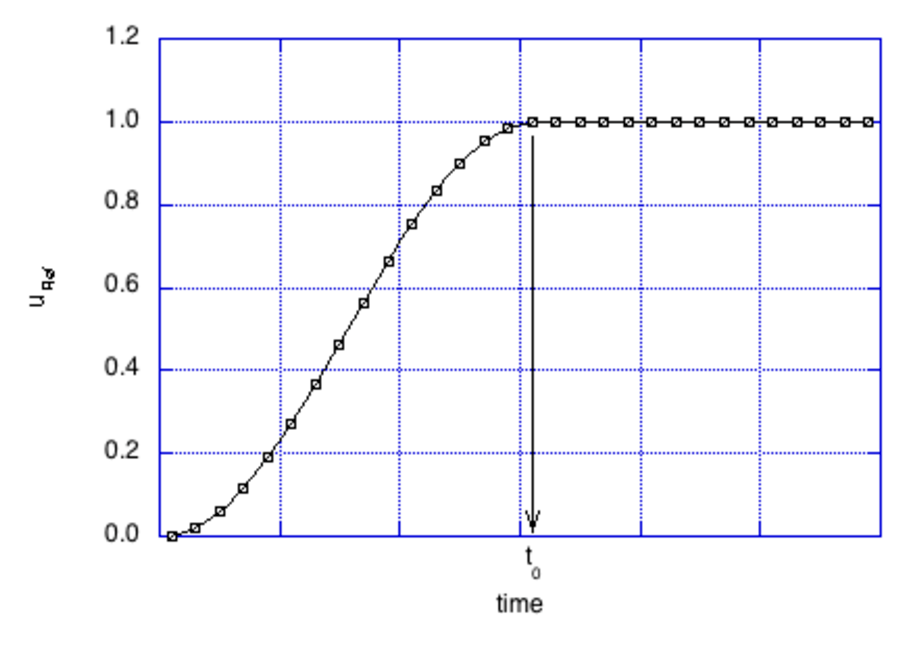
\includegraphics[width=7cm,clip]{accel_Velocity.eps}
\end{center}
\caption{加速中の速度プロファイル}
\label{fig:accel_velocity}
\end{figure}

%
\paragraph{時間積分幅$\Delta{t}$の指定}
\textbf{表\ref{tbl:delta t inc}}に時間積分幅\index{じかんせきぶんはば@時間積分幅}$\Delta{t}$の指定方法を示します.
拡散数\index{かくさんすう@拡散数}$D$は一次元の拡散方程式の場合$D=\alpha \delta t \slash h^2$で与えられます.$\alpha$は拡散係数で,Navier-Stokes方程式の場合$1/Re$,温度の輸送方程式の場合には$1/Pe$となります.安定性解析から$D<1 \slash 2$であることが要請されます.多次元の場合には,$d_m$を次元数として$\delta t<h^2 \slash (2d_m \alpha)$となります.

Delta\_tにはCFL数\index{CFL},または$\Delta t$を記述します.
時間積分幅の選択は,ソルバの種類を示すKind\_of\_Solverパラメータと関連があり,Solid\_Conductionの場合にはDt\_Directのみ選択できます.

\begin{table}[htdp]
\caption{Time\_Incrementのパラメータ指定}
\begin{center}
\small
\begin{tabular}{lll} \toprule
Dt\_Type & 時間積分幅の決定方法 & Delta\_tへの指定数値\\ \midrule
Direct & $\Delta t$を直接指定する & $\Delta t$\\
%CFL\_DFN\_MaxV & CFL\_MaxVと拡散数により制限される$\Delta t$の値の小さい方を選択\\
%CFL\_DFN\_RefV & CFL\_RefVと拡散数により制限される$\Delta t$の値の小さい方を選択\\
%CFL\_MaxV & CFL数を指定し,瞬時値の最大流速から$\Delta t$を決定 & CFL数\\
CFL\_Reference\_Velocity & CFL数を指定し,代表流速から$\Delta t$を決定 & CFL数\\
Diffusion & 拡散数から$\Delta t$を決定 & |\\
CFL\_Diffusion\_Reference\_Velocity & 代表流速に対するCFL数と拡散数から$\Delta t$を決定 & CFL数\\
%CFL\_MaxV\_CP & CFL数を指定し,音速を考慮した瞬時値の最大流速から$\Delta t$を決定 & CFL数\\
 \bottomrule
\end{tabular}
\end{center}
\label{tbl:delta t inc}
\end{table}

%
\pagebreak
\paragraph{計算時間の指定}
Period\_Typeで計算する時間の記述単位を指定します.
計算時間を時間で指定する場合,時間の単位は\hyperlink{tgt:unit}{Unit\_of\_Input\_Parameter}のモードに従います.
指定された単位の数値をCalculation\_Periodで指定します\footnote{SPHEREフレームワークでは,SPHERE定義要素としてCalculationStepsがありますが,内部的に上書きしています.}.

\end{indentation}



%%%
\pagebreak
\subsubsection{Treatment\_of\_Wall}

\hypertarget{tgt:treatment_of_wall}{壁面の扱い}について指定します.本パラメータは実験的実装です.

\begin{indentation}{3zw}{0zw}

{\small
\begin{program}
<Elem name="Treatment_of_Wall">
  <Param name="Pressure_Gradient" dtype="string" value="grad_zero"/>
  <Param name="Velocity_Profile"  dtype="string" value="no_slip"/>
</Elem>
\end{program}
}

各パラメータの意味について,\textbf{表\ref{tbl:wall_treatment}}に示します.
圧力勾配は法線方向の圧力勾配ゼロとNavier-Stokes方程式の圧力項を評価する2つの扱いが選択できます\footnote{現時点では,圧力勾配ゼロのみが選択できます.}.
速度プロファイルについては,滑りなし条件と壁関数を用いた近似が選択できます.壁関数は対数則が実装されています.詳細はCBCソルバークラス説明書をご覧ください\footnote{\today 未リリース.}.

\begin{table}[htdp]
\caption{壁面条件の指定}
\begin{center}
\small
\begin{tabular}{lll} \toprule
タグ & パラメータの値 & 説明\\ \midrule
Pressure\_Gradient & Grad\_Zero & 圧力勾配ゼロ\\
 & Grad\_NS & Navier-Stokes方程式から計算する\\ \hline
Velocity\_Profile  & No\_Slip & 滑りなし壁面条件\\
 & Slip & 滑り壁条件\\
 & Law\_of\_Wall & 壁法則\\ \bottomrule
\end{tabular}
\end{center}
\label{tbl:wall_treatment}
\end{table}

\end{indentation}


%%%
\pagebreak
\subsubsection{Unit}
\label{sec:p_unit}

入力ファイルと出力ファイルで用いる\hypertarget{tgt:unit}{単位を指定}します.

\begin{indentation}{3zw}{0zw}

{\small
\begin{program}
<Elem name="Unit">
  <Param name="Unit_of_Input_Parameter" dtype="STRING"  value="Dimensional" />
  <Param name="Pressure"                dtype="STRING"  value="gauge" />
  <Param name="Temperature"             dtype="STRING"  value="Celsius" />
</Elem>
\end{program}
}

各タグは,\textbf{表\ref{tbl:param_unit}}に示す単位の指定に用いられます.
有次元のファイル出力時には,圧力単位としてゲージ圧(Gauge Pressure)と絶対圧力(Absolute Pressure)が選択できます.
\textbf{式(\ref{eq:gauge pressure})}に示すゲージ圧を\textbf{式(\ref{eq:ND gauge})}により無次元化する場合に,基準圧として$p_0^\prime\,=\,1.0325\times 10^5$ [Pa]を用い,動圧が$10^0 \sim 10^3$程度とすると,$p \sim \mathrm{O}(1)$程度となるので,単精度計算では4桁程度有効桁が失われる場合もあります.
そのような場合,有次元値のファイル出力単位としてゲージ圧$p_g^\prime$を用います(非圧縮流れの場合には圧力差が意味をもつので,ゲージ圧でもかまいません).
ゲージ圧の基準となる大気圧$p_0^\prime\,$[Pa]は\hyperlink{tgt:reference}{Base\_Pressure}で指定します.
圧力単位の指定は,履歴ファイルのモニタ値にも適用されます.

\begin{equation}
p_g^\prime \,=\, p^\prime \,-\, p_0^\prime
\label{eq:gauge pressure}
\end{equation}

\begin{equation}
p \,=\, \frac{p_g^\prime}{\rho^\prime {u_0^\prime}^2}
\label{eq:ND gauge}
\end{equation}

\begin{table}[htdp]
\caption{単位の指定}
\begin{center}
\small
\begin{tabular}{lll} \toprule
タグ & 指定パラメータ & 説明\\ \midrule
Unit\_of\_Input\_Parameter & Dimensional or Non\_Dimensional & 入力パラメータファイルの単位を指定します(*1)\\
Pressure & Gauge or Absolute & 入力パラメータの単位が有次元のときに有効となります\\
Temperature & Celsius or Kelvin & 入力パラメータの単位が有次元のときに有効となります\\\bottomrule
\end{tabular}
\end{center}
\label{tbl:param_unit}
\end{table}

\end{indentation}



%%%
\pagebreak
\subsubsection{Version\_Info}

CBCソルバークラスとFlowBaseクラスの\hypertarget{tgt:version}{バージョン番号}を指定します.
異なる番号を指定している場合には,修正すべきバージョン番号が表示されるのでXMLファイルを変更します.

\begin{indentation}{3zw}{0zw}
\small
\begin{program}
<Elem name="Version_Info">
  <Param name="CBC"         dtype="INT"   value="127" />
  <Param name="Flow_Base"   dtype="INT"   value="225" />
</Elem>
\end{program}

\end{indentation}


%%%
\pagebreak
\subsubsection{VoxelDivisionMethod}
並列計算時の\hypertarget{tgt:voxel_division_method}{領域分割}をユーザーが明示的に指定します.直方体領域の計算空間を想定し,I, J, Kの各方向の分割数を指定します.
この指定が無い場合には,Sphereフレームワークがロードバランスが等しく,かつ通信面積が細小となる適切な分割を行います.

\begin{indentation}{3zw}{0zw}
\small
\begin{program}
<Elem name="VoxelDivisionMethod">
  <Param name="I"   dtype="INT"   value="8" />
  <Param name="J"   dtype="INT"   value="4" />
  <Param name="K"   dtype="INT"   value="5" />
</Elem>
\end{program}

\end{indentation}

%%% 隠しパラメータ
\begin{comment}
\subsubsection{Variable\_Range}

温度計算を実施する場合に,変数値を無次元値で[0,1]の範囲に\hypertarget{tgt:variable_range}{制限}することを指定します.

\begin{indentation}{3zw}{0zw}
\small

\begin{program}
<Param name="Variable_Range"     dtype="STRING" value="normal" />
\end{program}

\normalsize
温度の値に制限を課す場合に\textbf{表\ref{tbl:var_range}}に示すパラメータを使用します.保存則を満たさなくなるため,影響を考慮して利用してください.

\begin{table}[htdp]
\small
\caption{Variable\_Rangeのパラメータ指定}
\begin{center}
\begin{tabular}{ll} \toprule
タグ & モード\\ \midrule
cutoff & 値を無次元で[0, 1]に制限します\\
normal & 制限しません\\ \bottomrule
\end{tabular}
\end{center}
\label{tbl:var_range}
\end{table}

\end{indentation}
\end{comment}


%%%
\pagebreak
\subsection{Parameterセクション}
\label{sec:physical_parameter}

パラメータセクションでは,CBCソルバークラスの実行に必要な物理パラメータ\index{ぶつりぱらめーた@物理パラメータ}を記述します.



%%%
\subsubsection{Initial\_State}

\hypertarget{tgt:initial_state}{物理変数}の初期値\index{しょきち@初期値}を指定します.

\begin{indentation}{3zw}{0zw}

{\small
\begin{program}
<Elem name="Initial_State">
  <Param name="Density"     dtype="REAL" value="1.25e00" />
  <Param name="Pressure"    dtype="REAL" value="0.0" />
  <Param name="Temperature" dtype="REAL" value="20.0" />
  <Elem name="Velocity">
    <Param name="u" dtype="REAL" value="0.0"/>
    <Param name="v" dtype="REAL" value="0.0"/>
    <Param name="w" dtype="REAL" value="0.0"/>
  </Elem>
</Elem>
\end{program}
}

記述する初期値は有次元量で指定しますが,Solver\_Propertyセクションで\hyperlink{tgt:solver_property}{Kind\_of\_Solver}=\lq\lq Flow\_Only\rq\rq を指定した場合のみ,無次元での指定も可能です.
圧力値は,\hyperlink{tgt:unit}{Unit}で指定する圧力の単位に従います.
各変数の無次元化は以下のようになり,添え字の0は代表値または基準値を意味します.

\begin{equation}
\left.
\begin{array}{l}
\vspace{2mm}
\displaystyle{ \rho \,=\, \frac{\rho^{\prime}}{\rho_{0}^{\prime}} } \\
\vspace{2mm}
\displaystyle{ p \,=\, \frac{p^{\prime}-p_{0}^{\prime}}{\rho_{0}^{\prime}\,{u_{0}^{\prime}}^{2}} } \\
\vspace{2mm}
\displaystyle{ u_{i} \,=\, \frac{u_{i}^{\prime}}{u_0^{\prime}} } \\
\vspace{2mm}
\displaystyle{ \theta \,=\, \frac{\theta^{\prime}-\theta_{0}^{\prime}}{\Delta \theta^{\prime}} } 
\end{array} \qquad \right \}
\end{equation}

\end{indentation}

\vspace{3mm}
%%%
\subsubsection{Init\_Temp\_of\_Medium}
温度計算の場合に,割り当てた\hypertarget{tgt:initial_temp}{媒質}に対して初期温度を設定します.
媒質IDと流体・固体の種別は\hyperlink{tgt:model_setting}{Model\_Setting}と一致している必要があります.

{\small
\begin{program}
<Elem name="Init_Temp_of_Medium">
  <Param name="fluid" id="1"   dtype="real" value="20.0" />
  <Param name="solid" id="2"   dtype="real" value="34.0" />
  <Param name="solid" id="6"   dtype="real" value="34.0" />
  <Param name="solid" id="3"   dtype="real" value="35.0" />
  <Param name="fluid" id="4"   dtype="real" value="20.0" />
  <Param name="fluid" id="5"   dtype="real" value="20.0" />
  <Param name="fluid" id="10"  dtype="real" value="20.0" />
</Elem>
\end{program}
}

%%%
\pagebreak
\subsubsection{Intrinsic\_Example}

\hypertarget{tgt:intrinsic_example}{組み込み}例題\index{くみこみれいだい@組み込み例題}に固有のパラメータを指定します.

\begin{indentation}{3zw}{0zw}
\small

\begin{program}
<Elem name="Intrinsic_Example">
  ...
</Elem>
\end{program}

\normalsize
指定可能なパラメータは,\textbf{表\ref{tbl:intrinsic_parameter}}に示すように各\hyperlink{tgt:example}{組み込み例題}ごとに異なります.

\begin{table}[htdp]
\caption{Intrinsic\_Exampleセクションで指定できるパラメータ}
\begin{center}
\small
\begin{tabular}{llll} \toprule
組み込み例題 & 指定パラメータタグ & dtype & 指定値\\ \midrule
Duct3D & Shape     & STRING & Circular, Rectangular\\
       & Diameter  & REAL   & 断面径 [m]\\
       & Direction & STRING & X\_minus $|$ X\_plus $|$ Y\_minus $|$ Y\_plus $|$ Z\_minus $|$ Z\_plus\\
       & Driver    & REAL   & ドライバ部分の長さ [m]\\ \bottomrule
\end{tabular}
\end{center}
\label{tbl:intrinsic_parameter}
\end{table}

\end{indentation}



%%%
\pagebreak
\subsubsection{Reference}

解析に用いる無次元化の\hypertarget{tgt:reference}{基準量},あるいは無次元パラメータを指定します.

\begin{indentation}{3zw}{0zw}

{\small
\begin{program}
<Elem name="Reference">
  <Param name="Length"        dtype="REAL" value="1.0" />
  <Param name="Velocity"      dtype="REAL" value="1.0" />
  <Param name="Base_Pressure" dtype="REAL" value="101325" />
  <Param name="Gravity"       dtype="REAL" value="9.8" />
  <Param name="Reynolds"      dtype="REAL" value="1000.0" />
  <Param name="Prandtl"       dtype="REAL" value="0.71" />
  <Param name="Ref_ID"        dtype="INT"  value="1" />
</Elem>
\end{program}
}

\noindent \textbf{表\ref{tbl:ref_value}}に示すように基準量を必要に応じて記述できます.
無次元パラメータであるReynolds数とPrandtl数は,\hyperlink{tgt:unit}{Unit}の指定が無次元のときのみ指定できます.
Ref\_IDで指定するIDは,ボクセルモデル内で使われ,かつ\hyperlink{tgt:model_setting}{Model\_Setting}セクションで記述されている必要があります.固体熱伝導解析の場合には固体のIDを指定し,それ以外の(熱)流動解析の場合には流体のIDを指定します.

\begin{table}[htdp]
\caption{Referenceセクションで指定できるパラメータ}
\begin{center}
\small
\begin{tabular}{llll} \toprule
値 & 意味 & 単位\\ \midrule
Length & 代表長さ & $m$ &\\
Velocity & 代表速度 & $m/s$ &\\
Base\_Pressure & 基準圧力 & $Pa$ &\\
Gravity & 重力加速度 & $m^2/s$ &\\
%Grashof & グラショフ数 & |\\
Prandtl & プラントル数 & | & 無次元のときのみ指定\\
%Rayleigh & レイリー数 & |\\
Reynolds & レイノルズ数 & | & 無次元のときのみ指定\\
Ref\_ID & 代表物性値として指定する媒質ID & | &\\ \bottomrule
\end{tabular}
\end{center}
\label{tbl:ref_value}
\end{table}

\end{indentation}



%%%
\pagebreak
\subsubsection{Temperature}

\hypertarget{tgt:temperature}{温度計算}を実施する場合の基準量を有次元値で指定します.

\begin{indentation}{3zw}{0zw}

{\small
\begin{program}
<Elem name="Temperature">
  <Param name="Base"       dtype="REAL"   value="293.15" />
  <Param name="Difference" dtype="REAL"   value="35.0" />
</Elem>
\end{program}
}

基準温度(Base)と温度差(Difference)は,非圧縮計算のパッシブスカラーによる温度計算では温度場を特徴づける代表量となります.
単位は\hyperlink{tgt:unit}{Temperature}タグで指定します.

\end{indentation}



%%%
\pagebreak
\subsection{Medium\_Tableセクション}

ソルバーで利用する媒質の\hypertarget{tgt:medium_table}{物性値テーブル}を記述します.
ここで記述する媒質の基本リスト\index{きほんりすと@基本リスト!ばいしつの@媒質の---}は,解析に利用される候補です.
媒質は流体と固体が記述でき,\textbf{表\ref{tbl:MTLentry}}により媒質を指定します.

\begin{indentation}{3zw}{0zw}

{\small
\begin{program}
<Medium_Table>
  <Elem name="Fluid" id="100" comment="Air">
    <Param name="density"              dtype="REAL" value="1.1763" />
    <Param name="specific_heat"        dtype="REAL" value="1007" />
    <Param name="thermal_conductivity" dtype="REAL" value="2.614e-02" />
    <Param name="kinematic_viscosity"  dtype="REAL" value="15.83e-06" />
    <Param name="viscosity"            dtype="REAL" value="18.62e-06" />
    <Param name="sound_of_speed"       dtype="REAL" value="340.0" />
    <Param name="volume_expansion"     dtype="REAL" value="0.04e-3" />
  </Elem>
  <Elem name="Solid" id="600" comment="Fe">
    <Param name="density"              dtype="REAL" value="7870.0" />
    <Param name="specific_heat"        dtype="REAL" value="442.0" />
    <Param name="thermal_conductivity" dtype="REAL" value="80.3" />
  </Elem>
</Medium_Table>
\end{program}
}

\begin{table}[htdp]
\caption{Medium\_Tableに記述するパラメータ}
\begin{center}
\begin{tabular}{ll} \toprule
タグ & 説明\\ \midrule
Elem name & Fluid または Solid\\
ID & 媒質ID\\
comment & 媒質名\\ \bottomrule
\end{tabular}
\end{center}
\label{tbl:MTLentry}
\end{table}


各媒質は固体と流体によって記述しなければならない物性値が異なります.
指定できる項目を\textbf{表\ref{tbl:medium_tbl}}に示します.
固体については,密度・比熱・熱伝導率のみの記述となります.
各媒質の情報は,任意に指定するID番号によって管理されます.

\begin{table}[htdp]
\caption{Medium\_Tableにおける物性値の指定}
\begin{minipage}{.45\textwidth}
\begin{center}
\begin{tabular}{lll}\\ \toprule
Fluidのキーワード & 説明 & 単位\\ \midrule
Density & 密度 & $kg/m^3$\\
Specific\_Heat & 定圧比熱 & $kJ/(kg K)$\\
Thermal\_Conductivity & 熱伝導率 & $W/(m K)$\\
Kinematic\_Viscosity & 動粘性係数 & $m^2/s$\\
Viscosity & 粘性係数 & $Pa\,s$\\
Sound\_of\_Speed & 音速 & $m/s$\\
Volume\_Expansion & 体膨張率 & $1/K$\\ \bottomrule
\end{tabular}
\end{center}
\end{minipage} \hfill
\begin{minipage}{.45\textwidth}
\begin{center}
\begin{tabular}{lll}\\ \toprule
Solidのキーワード & 説明 & 単位\\ \midrule
Density & 密度 & $kg/m^3$\\
Specific\_Heat & 定圧比熱 & $kJ/(kg K)$\\
Thermal\_Conductivity & 熱伝導率 & $W/(m K)$\\ \bottomrule
\end{tabular}
\end{center}
\end{minipage}
\label{tbl:medium_tbl}
\end{table}

\end{indentation}





%%%
\chapter{境界条件}
\label{chpt:BC}
\begin{abstract}
本章では,CBCソルバークラスで設定できる境界条件の設定について説明します.
まず境界条件と媒質を指定するXMLタグの構造について述べた後,流れと熱の境界条件について説明します.
\end{abstract}
%
\graphicspath{{./fig_BC/}}

%
\section{境界条件の概要}

%
\hypertarget{tgt:BC policy}{\subsection{外部境界条件と内部境界条件}}
CBCソルバークラスでは,境界条件を外部境界条件と内部境界条件の2つに分けて指定します.
外部境界条件は計算領域外部面に指定する境界条件で,内部境界条件は計算領域内部に指定する境界条件です.
\textbf{図\ref{fig:BCs}}に示すように,計算領域を構成する6面が外部境界面で,この部分に与える境界条件が外部境界条件です.
それ以外の内部領域(セル体積とセルフェイス)に作用する境界条件は内部境界条件として扱います.
外部境界面には,外部境界条件が各面に対して1種類のみ与えることができ,内部境界条件を適用することはできません.

\begin{figure}[htbp]
\begin{center}
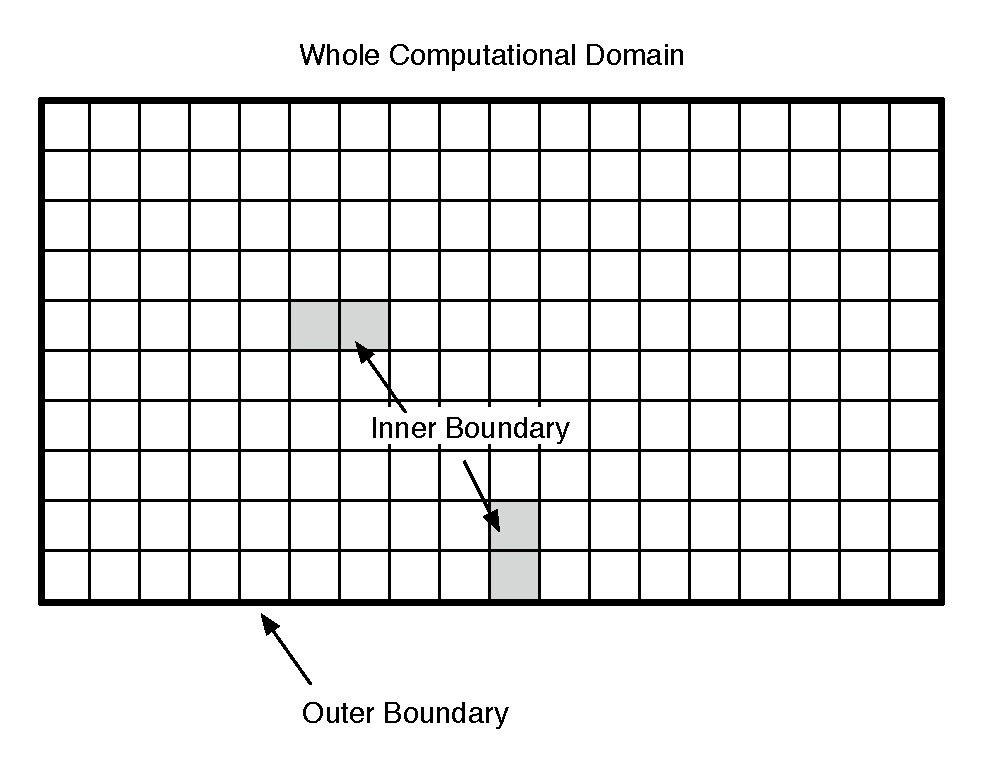
\includegraphics[width=10cm,clip]{Boundary.eps}
\end{center}
\caption{計算領域における外部境界と内部境界の指定場所}
\label{fig:BCs}
\end{figure}

%
\subsection{BC\_TableセクションのXML構造}
境界条件を記述するBC\_Tableセクションは,SphereConfig\index{SphereConfig}内に記述しても良いし,独立したファイルに記述しても構いません.独立ファイルとして扱う場合には,DomainInfo\index{DomainInfo}セクションで次のように外部ファイルとして記述します.valueには,V-Sphereを起動するディレクトリからの相対パスとなるように記述しておきます.

{\small
\begin{program}
<Param name="BCTBL" dtype="STRING" value="xml/boundary.xml"/>
\end{program}
}

BC\_Tableセクションでは,次のように内部境界条件InnerBoundary\index{InnerBoundary}と外部境界条件OuterBoundary\index{OuterBoundary}の2つを記述します.

{\small
\begin{program}
<BC_Table>
  <OuterBoundary>
    <Elem name="Basic_BCs">
      <Elem name="Wall" id="1">
        <Param name="Normal_x"         dtype="REAL"   value="0.0" />
        <Param name="Normal_y"         dtype="REAL"   value="0.0" />
        <Param name="Normal_z"         dtype="REAL"   value="0.0" />
        <param name="Profile"          dtype="STRING" value="Constant" />
        <param name="Specified_Type"   dtype="STRING" value="Velocity" />
        <Param name="Specified_Value"  dtype="REAL"   value="7.0" />
      </Elem>
      
      <Elem name="outflow" id="3">
        <Param name="velocity_type"  dtype="STRING" value="Average" />
      </Elem>
      
      <Elem name="periodic" id="10" >
        <Param name="mode"             dtype="string" value="driver" />
        <Param name="driver_direction" dtype="string" value="x_minus" />
      </Elem>
    </Elem>
    
    <Elem name="Face_BC">
      <Elem name="X_MINUS" id="10" comment="periodic">
        <Param name="Guide_Cell_ID" id="1" />
      </Elem>
      <Elem name="X_PLUS"  id="3" comment="outflow">
        <Param name="Guide_Cell_ID" id="2" />
      </Elem>
      <Elem name="Y_MINUS" id="1" comment="wall">
        <Param name="Guide_Cell_ID" id="2" />
      </Elem>
      <Elem name="Y_PLUS"  id="1" comment="wall">
        <Param name="Guide_Cell_ID" id="2" />
      </Elem>
      <Elem name="Z_MINUS" id="1" comment="wall">
        <Param name="Guide_Cell_ID" id="2" />
      </Elem>
      <Elem name="Z_PLUS"  id="1" comment="wall">
        <Param name="Guide_Cell_ID" id="2" />
      </Elem>
    </Elem>
  </OuterBoundary>
</BC_Table>
\end{program}
}


%
\hypertarget{tgt:outer_boundary}{\subsection{OuterBoundary}}

計算領域の外部境界条件を次の方針により指定します.

\begin{enumerate}
\item 候補となる境界条件の種類をBasic\_BCsタグ内にリストアップし,基本リストを作成します.境界条件の基本リスト\index{きほんりすと@基本リスト!きょうかいじょうけんの@境界条件の---}には,ユニークなID(番号)を割り振ります.
\item Face\_BCタグ内において,境界条件の基本リストのIDを参照し,計算領域の外部境界の各面における境界条件を指定します.同時に,各面のガイドセルのセルIDをGuide\_Cell\_IDにより指定します.
\end{enumerate}

前述の例では,境界条件の候補としてID=1, 3, 10をリストアップしています.Xマイナス方向の外部境界面に周期境界条件(ID=10)を与え,Xプラス方向の外部境界面に流出境界条件(ID=3),それ以外の面には壁面条件(ID=1)を与えています.各外部境界面のガイドセルにはGuide\_Cell\_IDによって,IDを付与しています.このIDは,\hyperlink{tgt:model_setting}{Model\_Setting}セクションにリストアップされたIDを参照します.
外部境界条件は,計算領域を構成する外部境界面の各面ごとに一様な境界条件となります.

指定できる境界条件の種類を\textbf{表\ref{tbl:outer BC physical}}に示します.
熱流れの場合には,壁面境界の場合に細かい指定が可能です.

\begin{table}[htdp]
\caption{外部境界で指定できる流れと熱の境界条件の種類}
\begin{center}
\small
\begin{tabular}{ll|ll} \toprule
流れの境界指定のキーワード &  流れの境界条件 & 熱境界指定のサブキーワード & 熱境界条件\\ \midrule
In\_Out & 流入出境界 & Ambient\_Temperature & 流入温度指定と対流流出\\
Outflow & 流出境界 & $\leftarrow$ & 対流流出\\
Periodic & 周期境界 & $\leftarrow$ & 周期境界\\
Specified\_Velocity & 流入境界 & Temperature & 流入温度指定\\
Symmetric & 対称境界 & $\leftarrow$ & 対称境界\\
Traction\_Free & 遠方境界 & Ambient\_Temperature & 遠方温度指定\\ \hline
Wall & 壁面境界 & Adiabatic & 断熱指定\\
& & HeatFlux & 熱流束指定\\ 
& & HeatTransfer Type\_S & 熱伝達係数と表面温度から熱伝達を計算\\
& & HeatTransfer Type\_SF & 強制対流の層流・乱流熱伝達境界\\
& & HeatTransfer Type\_SN & 自然対流の乱流熱伝達境界\\
& & HeatTransfer Type\_B & 固体壁からの放熱条件\\
& & IsoThermal & 等温指定\\
\bottomrule
\end{tabular}
\end{center}
\label{tbl:outer BC physical}
\end{table}


%
\pagebreak
\hypertarget{tgt:innerboundary}{\subsection{InnerBoundary}}

計算領域内の境界条件を記述するセクションで,\textbf{表\ref{tbl:tag_ibc}}に示す種類を指定できます.
CBCソルバークラスは,内部境界条件をコンポーネント\index{コンポーネント}として扱います.
内部境界条件を指定する位置には,ボクセルのセル要素に対して作用するものとセル界面に作用する2種類のコンポーネントがあります.

内部境界条件の位置は,外部境界面を除く計算領域内に対して,ボクセルモデルのセルIDにより指定します.
境界条件の詳細は,XMLのInnerBoundaryセクションのID番号に記述します.
内部境界条件で指定する各コンポーネントの個数と実際の解析モデル中のコンポーネントの個数は一致している必要があります.
\textbf{指定できる内部境界条件の数は30個が上限}です.
また,\textbf{指定境界条件数と媒質数の和は63個以下}となります\footnote{これらの制限は,境界条件を効率よく実装する方法の制約から来るものです.}.

Inactiveタグは,計算空間内で計算しない不活性セルを指定します.
Cell\_Monitorは境界条件ではありませんが,同じ仕組みを用いて実装しているので,このセクションに設けています.




\begin{table}[htdp]
\caption{内部境界条件(コンポーネント)の種類}
\begin{center}
\small
\begin{tabular}{lllll} \toprule
タグ & 指定位置 & 計算モード & 実装形式 & コンポーネントの説明\\ \midrule
Specified\_Velocity & セル界面 & 流れ・熱流れ & 対流流束 & 速度指定境界\\
Outflow & セル界面 & 流れ・熱流れ & 対流流束 & 流出境界\\
Periodic & セル界面 & 流れ・熱流れ & 参照値指定 & 部分周期境界\\
%FORCING & Direct ForcingによるImmersed Boundary境界条件\\
%HEX & 熱交換器\\
%FAN & ファン\\
%DARCY & ダルシー則\\
Inactive & セル要素 & 流れ・熱流れ & マスク & 不活性化する計算空間内のセルIDを指定\\
Cell\_Monitor & セル要素 & 流れ・熱流れ & - & 物理量のモニター位置の指定\\ 
Adiabatic & セル界面 & 熱流れ & 熱流束マスク & 断熱セル指定\\
Direct\_Heat\_Flux & セル界面 & 熱流れ & 熱流束 & 熱流束指定\\
HeatTransfer\_B & セル界面 & 固体伝熱 & 熱流束 & 固体壁からの放熱条件\\
HeatTransfer\_S & セル界面 & 熱流れ & 熱流束 & 熱伝達係数と表面温度により計算\\
%HeatTransfer\_N & セル界面 & 熱 & 熱流束 & 熱伝達形式\\
HeatTransfer\_SF & セル界面 & 熱流れ & 熱流束 & 強制対流の層流・乱流熱伝達境界\\
HeatTransfer\_SN & セル界面 & 熱流れ & 熱流束 & 自然対流の乱流熱伝達境界\\
IsoThermal & セル界面 & 熱流れ & 熱流束 & 等温面指定\\
Heat\_Source & セル要素 & 熱流れ & 外力項 & 吸発熱指定\\
Specified\_Temperature & セル要素 & 熱流れ & 温度指定 & セルの温度指定\\
\bottomrule
\end{tabular}
\end{center}
\label{tbl:tag_ibc}
\end{table}


%
\pagebreak
\hypertarget{tgt:grid_arrangement}{\subsection{計算格子と内部・外部領域}}

非圧縮性流体の境界条件で参照する計算領域と格子配置について説明します.
計算領域とコロケート変数配置\index{へんすうはいち@変数配置!コロケート@Collocated---}の変数のインデクス\index{インデクス}の表記を\textbf{図\ref{fig:index_domain}},\textbf{図\ref{fig:index_cc}}に示します.

\begin{figure}[htdp]
  \begin{center}
  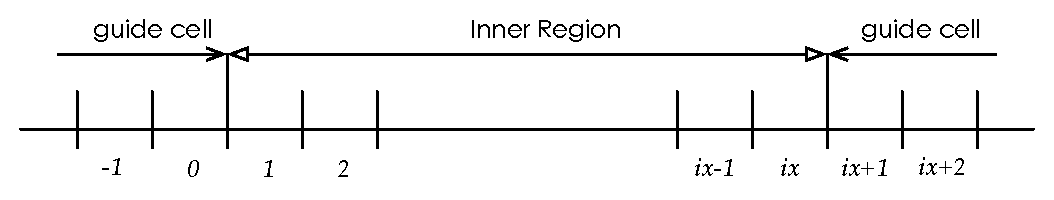
\includegraphics[width=12cm,clip]{index_domain.eps}
  \end{center}
  \caption{計算領域のインデクス}
  \label{fig:index_domain}
\end{figure}

\begin{figure}[htdp]
  \begin{center}
  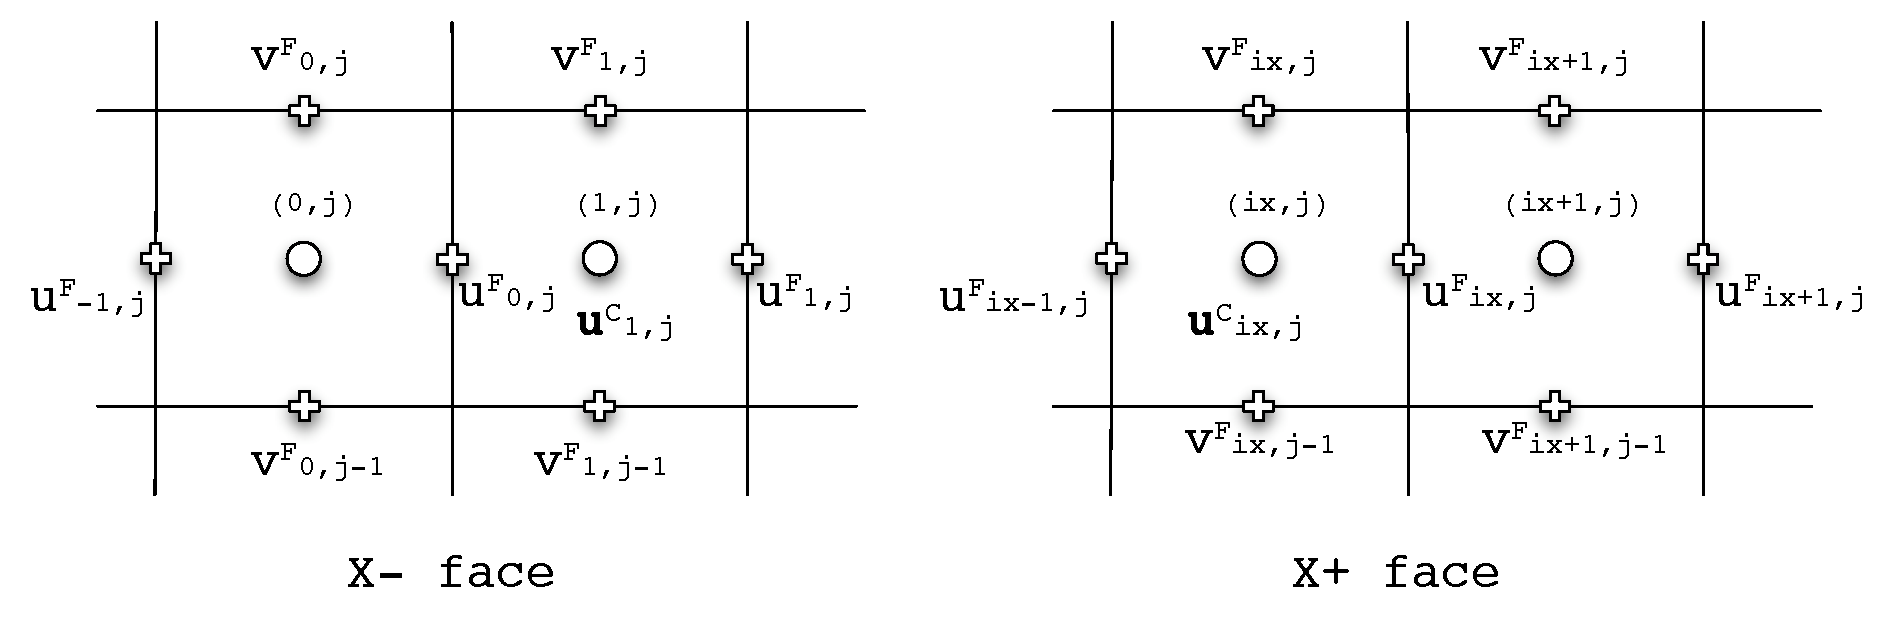
\includegraphics[width=14cm,clip]{index_cc.eps}
  \end{center}
  \caption{コロケート配置の変数のインデクス.基本変数($u_{\,i}^{\,C},\, p,\,\theta$)は全てセルセンタ位置に配置され,補助的な速度ベクトル$u_{\,i}^{\,F}$がスタガード位置に配置されます.}
  \label{fig:index_cc}
\end{figure}


%%%
\pagebreak
\section{外部境界条件}

%
\subsection{壁面境界}

\subsubsection{流れの境界条件}

壁面の速度境界条件では,指定する境界面の移動速度を与えます.
壁面速度が時間的に変化する場合と一定の場合があります.
ただし,壁面速度ベクトルは壁面と平行なスライド成分のみで,壁面と垂直な成分はゼロである点に注意します.

壁面境界は,与えられた速度からセルフェイス位置の運動量流束を計算して,運動量流束を直接与えます.
外部境界では下記のようなXML入力パラメータで指定します.
次の境界条件の例では,Y方向に7[m/s],2[Hz]で平行振動する壁の境界条件を指定しています.

{\small
\begin{program}
<OuterBoundary>
  <Elem name="Basic_BCs">
    <Elem name="wall" id="1">
      <Param name="Normal_x"        dtype="REAL"   value="0.0" />
      <Param name="Normal_y"        dtype="REAL"   value="1.0" />
      <Param name="Normal_z"        dtype="REAL"   value="0.0" />
      <param name="Profile"         dtype="STRING" value="Harmonic" />
      <param name="Specified_Type"  dtype="STRING" value="Velocity" />
      <Param name="Specified_Value" dtype="REAL"   value="7.0" />
      <Param name="Frequency"       dtype="REAL"   value="2.0" />
      <Param name="Initial_Phase"   dtype="REAL"   value="0.0" />
      <Param name="Constant_Bias"   dtype="REAL"   value="0.0" />
    </Elem>
  </Elem>
</OuterBoundary>
\end{program}
}

\begin{table}[htdp]
\caption{壁面の速度境界条件の指定パラメータ}
\begin{center}
\small
\begin{tabular}{lll} \toprule
タグ & 指定キーワード & パラメータの説明\\ \midrule
Normal\_x & | & 法線ベクトルのx方向成分\quad 法線は単位ベクトル\\
Normal\_y & | & 法線ベクトルのy方向成分\\
Normal\_z & | & 法線ベクトルのz方向成分\\
Profile & Constant $|$ Harmonic & 指定速度のタイプ\\
Specified\_Type & Velocity & 指定単位 $[m/s]$\\
Specified\_Value & | & 速度\\
Frequency & | & 周波数 $f\, [Hz]$\\
Initial\_Phase & | & 初期位相 $\phi\, [Rad]$\\
Constant\_Bias & | & 一定値 $b\, [m/s]$\\
\bottomrule
\end{tabular}
\end{center}
\label{tbl:wall parameter out}
\end{table}

壁面の速度境界の指定パラメータを\textbf{表\ref{tbl:wall parameter out}}に示します.
時間変化を伴う速度指定はProfile=\lq\lq Harmonic\rq\rq を指定し,\textbf{式(\ref{eq:harmonic out})}の形式の単振動\index{たんしんどう@単振動}の境界条件を周期や初期位相,固定バイアスと供に与えます.時間的に変化しない壁面境界の場合にはProfile=\lq\lq Constant\rq\rq を指定し,周波数,初期位相,固定バイアス値の指定は不要です.

\begin{equation}
V \,{=}\, A \sin \left( 2 \mathrm{\pi} ft \,+\, \phi \right) \,+\, b
\label{eq:harmonic out}
\end{equation}


壁面境界に対する圧力の境界条件は,Navier-Stokes方程式からNeumann型の圧力境界条件が得られます.
高レイノルズ数流れにおいては,粘性項の寄与が小さいと仮定し粘性項を省略し$\nabla p=0$の形式になります.
圧力の壁面境界条件については,内部と外部の扱いは同じで,スキーム中で壁面を認識し$\nabla p=0$が満たされるようになっていますので,明示的な境界条件の指定は必要ありません.

%
\subsubsection{熱境界条件}
計算領域の外部面における壁面に対する熱境界条件としては,断熱,熱流束,熱伝達,等温が指定できます.
熱伝達境界は,さらに幾つかの指定パターンがあります.
詳細は\verb|Inside_CBC.pdf|をご覧ください.

%
\paragraph{断熱境界}
熱流束がゼロ,つまり$q^{\prime}=0$を指定します.
下記の例では,固定壁(壁面速度がゼロ)で,断熱条件を指定しています.

{\small
\begin{program}
<OuterBoundary>
  <Elem name="Basic_BCs">
    <Elem name="wall" id="1">
      <Param name="Normal_x"        dtype="REAL"   value="0.0" />
      <Param name="Normal_y"        dtype="REAL"   value="1.0" />
      <Param name="Normal_z"        dtype="REAL"   value="0.0" />
      <param name="Profile"         dtype="STRING" value="Constant" />
      <param name="Specified_Type"  dtype="STRING" value="Velocity" />
      <Param name="Specified_Value" dtype="REAL"   value="0.0" />
      <Param name="Heat_Type"       dtype="STRING" value="Adiabatic" />
    </Elem>
  </Elem>
</OuterBoundary>
\end{program}
}

%
\paragraph{熱流束境界}
境界面で指定の熱流束$q^{\prime}[W/m^2]$を与えます.
符号は計算領域内に流入する熱流束の場合に正,流出する熱流束の場合に負とします.
下記の例ではid=1の条件として,$12.0[W/m^2]$で流入する熱流束をもつ面を指定しています.

{\small
\begin{program}
<OuterBoundary>
  <Elem name="Basic_BCs">
    <Elem name="wall" id="1">
      ...
      <Param name="Heat_Type"       dtype="STRING" value="HeatFlux" />
      <Param name="Heat_Flux"       dtype="REAL"   value="12.0" />
    </Elem>
  </Elem>
</OuterBoundary>
\end{program}
}


%
\hypertarget{tgt:heat-transfer}{\paragraph{熱伝達境界}}
熱伝達境界は次式の形式で熱流束を与える条件で,幾つかの種類があります.
熱流体解析のモードと指定できる熱伝達境界の関係を\textbf{表\ref{tbl:type of HT}}に示します.

\begin{table}[htdp]
\caption{熱伝達境界条件とKind\_of\_Solverの関係}
\begin{center}
\small
\begin{tabular}{ll} \toprule
KIND\_OF\_SOLVER & 指定できる熱伝達境界の種類\\ \midrule
FLOW\_ONLY & -\\
THERMAL\_FLOW $|$ THERMAL\_FLOW\_NATURAL & Type\_S $|$ Type\_SN $|$ Type\_SF\\
CONJUGATE\_HEAT\_TRANSFER & Type\_N\\
SOLID\_CONDUCTION & Type\_B\\ \bottomrule
\end{tabular}
\end{center}
\label{tbl:type of HT}
\end{table}


\begin{equation}
q^{\prime} \,=\, -H(\theta_{sf}^{\prime}\,-\,\theta_{\infty}^{\prime})
\label{eq:ht form}
\end{equation}

\begin{center}
\begin{tabular}{lll}
$H$ &  $[W\,/\,(m^2K)]$ & Coefficient\, of\, heat\, transfer\\
$\theta_{sf}^{\prime}$ & $[K]$ & Surface\, temperature\, of\, solid\\
$\theta_{\infty}^{\prime}$ & $[K]$ & Temperature\, at\, outer\, boundary\, layer\\
\end{tabular}
\end{center}

\vspace{5mm}
\begin{indentation}{3zw}{0zw}

%
\subparagraph{Type\_S  表面温度と熱伝達係数により計算}
Type\_Sは表面温度と熱伝達係数を与え,熱流束を計算します.
\textbf{式(\ref{eq:ht form})}において,熱伝達係数$H$と固体表面温度$\theta_{sf}^{\prime}$を与え,\textbf{図\ref{fig:HT_Type_S}}に示す固体表面に隣接する流体セルの値を$\theta_{\infty}^{\prime}$として,界面での熱流束を計算します.

\begin{figure}[htdp]
\begin{center}
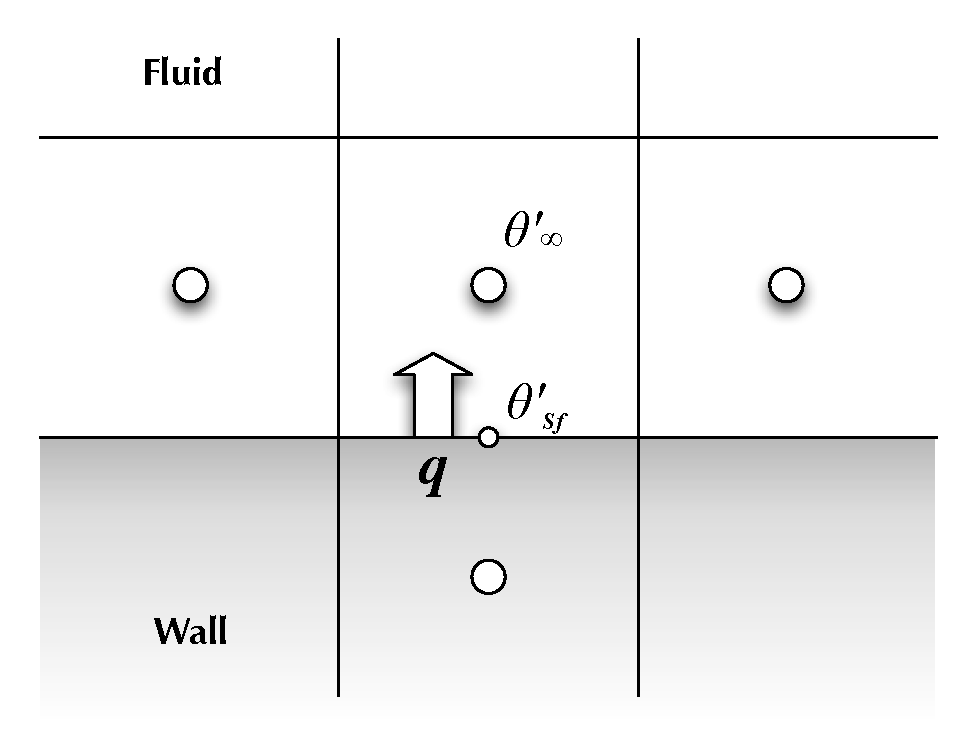
\includegraphics[width=7cm,clip]{HeatTransfer_Type_S.eps}
\end{center}
\caption{Type\_Sの熱伝達境界}
\label{fig:HT_Type_S}
\end{figure}

以下に,熱境界部分のみパラメータ指定の一例を示します.

{\small
\begin{program}
<OuterBoundary>
  <Elem name="Basic_BCs">
    <Elem name="wall" id="1">
      ...
      <Param name="Heat_Type"             dtype="STRING" value="HeatTransfer_S" />
      <Param name="Surface_Temperature"   dtype="REAL"   value="300.0"/>
      <Param name="Coef_of_Heat_Transfer" dtype="REAL"   value="20.0"/>
    </Elem>
  </Elem>
</OuterBoundary>
\end{program}
}

\begin{table}[htdp]
\caption{熱伝達境界Type\_Sの指定パラメータ}
\begin{center}
\small
\begin{tabular}{ll} \toprule
指定キーワード & パラメータの説明\\ \midrule
Coef\_of\_Heat\_Transfer & 熱伝達係数$[W/(m^2K)]$\\
Surface\_Temperature & 表面温度$[K\,|\,{}^\circ\mathrm{C}]$\\
\bottomrule
\end{tabular}
\end{center}
\label{tbl:hts}
\end{table}

%
\subparagraph{Type\_SN  自然対流の乱流熱伝達}
自然対流の場合の乱流熱伝達の実験式を実装した境界条件です.
文献\cite{shouji:95:Dennetsu}には,平板に対する自然対流の層流と乱流の熱伝達に関する近似式が説明されています.
雰囲気流体の温度に比べ加熱面の温度が非常に高い場合,平板が長くなると境界層が不安定になり,ほぼ$Ra>10^9$で層流から乱流へ遷移します.
垂直平板に関する平均熱伝達$(\overline{Nu_L},代表長L)$は次式で整理されます.

\begin{equation}
\left.
\begin{array}{lll}
\vspace{1mm}
層流 & \overline{Nu_L} \,=\, 0.59Ra_L^{1/4} & (10^4 < Ra_L < 10^9)\\
乱流 & \overline{Nu_L} \,=\, 0.10Ra_L^{1/3} & (10^9 < Ra_L < 10^{13})
\end{array} \right\}
\label{eq:natural_convection_vert_ht}
\end{equation}

一方,水平平板の場合には,加熱面が上面と下面にある場合で雰囲気流体の挙動が異なるため,\textbf{式(\ref{eq:natural_convection_horiz_ht})}のように整理されています.

\begin{equation}
\left.
\begin{array}{lll}
\vspace{1mm}
上面加熱 & \overline{Nu_L} \,=\, 0.54Ra_L^{1/4} & (10^4 < Ra_L < 10^7)\\
\vspace{1mm}
上面加熱 & \overline{Nu_L} \,=\, 0.15Ra_L^{1/3} & (10^7 < Ra_L < 10^{11})\\
\vspace{1mm}
下面加熱 & \overline{Nu_L} \,=\, 0.27Ra_L^{1/4} & (10^5 < Ra_L < 10^{10})
\end{array} \right\}
\label{eq:natural_convection_horiz_ht}
\end{equation}

上式を形式的にまとめると,

\begin{equation}
H \,=\, \alpha Ra_L^\beta \frac{\lambda}{L^\prime}
\label{eq:typeSN_form_ht}
\end{equation}

Type\_SNの境界条件は,上式のパラメータを実装しています.ここでは,垂直平板と水平平板の上面は,同じ係数を用いています.

{\small
\begin{program}
<OuterBoundary>
  <Elem name="Basic_BCs">
    <Elem name="wall" id="1">
      ...
      <Param name="Heat_Type"                dtype="STRING" value="HeatTransfer_SN" />
      <Param name="Surface_Temperature"      dtype="REAL"   value="500.0"/>
      <Param name="Ref_Temp_Mode"            dtype="STRING" value="Bulk_Temperature"/>
      <Param name="vertival_laminar_alpha"   dtype="REAL"   value="0.59"/>
      <Param name="vertival_laminar_beta"    dtype="REAL"   value="0.25"/>
      <Param name="vertival_turbulent_alpha" dtype="REAL"   value="0.1"/>
      <Param name="vertival_turbulent_beta"  dtype="REAL"   value="0.3333333"/>
      <Param name="vertival_ra_critial"      dtype="REAL"   value="1.0e9"/>
      <Param name="lower_laminar_alpha"      dtype="REAL"   value="0.27"/>
      <Param name="lower_laminar_beta"       dtype="REAL"   value="0.25"/>
      <Param name="lower_turbulent_alpha"    dtype="REAL"   value="0.27"/>
      <Param name="lower_turbulent_beta"     dtype="REAL"   value="0.25"/>
      <Param name="lower_ra_critial"         dtype="REAL"   value="1.0e9"/>
    </Elem>
  </Elem>
</OuterBoundary>
\end{program}
}

\begin{table}[htdp]
\caption{熱伝達境界Type\_SNのパラメータ}
\begin{center}
\small
\begin{tabular}{ll}\toprule
パラメータタグ & 記号の意味\\ \midrule
Vertival\_Laminar\_Alpha & 垂直平板と水平平板(上面)の層流時の係数$\alpha$\\
Vertival\_Laminar\_Beta & 垂直平板と水平平板(上面)の層流時の係数$\beta$\\
Vertival\_Turbulent\_Alpha & 垂直平板と水平平板(上面)の乱流時の係数$\alpha$\\
Vertival\_Turbulent\_Beta & 垂直平板と水平平板(上面)の乱流時の係数$\beta$\\
Vertival\_Ra\_Critial & 垂直平板と水平平板(上面)の臨界Ra数$Ra_L$\\
Lower\_Laminar\_Alpha & 水平平板(下面)の層流時の係数$\alpha$\\
Lower\_Laminar\_Beta & 水平平板(下面)の層流時の係数$\beta$\\
Lower\_Turbulent\_Alpha & 水平平板(下面)の乱流時の係数$\alpha$\\
Lower\_Turbulent\_Beta & 水平平板(下面)の乱流時の係数$\beta$\\
Lower\_Ra\_Critial & 水平平板(下面)の臨界Ra数$Ra_L$\\ 
Ref\_Temp\_Mode & Bulk\_Temperature or Local\_Temperature\\ \bottomrule
\end{tabular}
\end{center}
\label{tbl:htsn}
\end{table}


%
\subparagraph{Type\_SF  強制対流の層流・乱流熱伝達}
強制対流の場合の層流・乱流熱伝達の実験式を実装した境界条件です.
文献\cite{shouji:95:Dennetsu}から,平板に対する発達した強制対流の乱流熱伝達は,実験による摩擦係数の測定結果とチルトン-コルバーンのアナロジーを用い,温度一定で平板が遷移長さよりも十分に大きいと仮定すると,\textbf{式(\ref{eq:forced_convection_ht})}のように表せます.
実験式を整理すると,熱伝達係数は以下のような表現ができます.

\begin{equation}
\overline{Nu_L} \,=\, 0.037Re_L^{4/5}Pr^{1/3}
\label{eq:forced_convection_ht}
\end{equation}

形式的に次式のように表し,パラメータを求めます.

\begin{equation}
H \,=\, \alpha Re_L^\beta \, Pr^\gamma \, \frac{\lambda}{L^\prime}
\label{eq:typeSF_form_ht}
\end{equation}


温度差の定義にはバルク温度と隣接セルの値を用いたオプションが選択できます.
以下に,パラメータ指定の一例を示します.

{\small
\begin{program}
<OuterBoundary>
  <Elem name="Basic_BCs">
    <Elem name="wall" id="1">
      ...
      <Param name="Heat_Type"           dtype="STRING" value="HeatTransfer_SF" />
      <Param name="Surface_Temperature" dtype="REAL"   value="500.0"/>
      <Param name="Ref_Temp_Mode"       dtype="STRING" value="Bulk_Temperature"/>
      <Param name="alpha"               dtype="REAL"   value="0.037"/>
      <Param name="beta"                dtype="REAL"   value="0.8"/>
      <Param name="gamma"               dtype="REAL"   value="0.333333"/>
    </Elem>
  </Elem>
</OuterBoundary>
\end{program}
}

\begin{table}[htdp]
\caption{熱伝達境界Type\_SFのパラメータ}
\begin{center}
\small
\begin{tabular}{ll}\toprule
タグ & 記号の意味\\ \midrule
alpha & \textbf{式(\ref{eq:typeSF_form_ht})}中の係数$\alpha$\\
beta & 係数$\beta$\\
gamma & 係数$\gamma$\\
Ref\_Temp\_Mode & Bulk\_Temperature or Local\_Temperature\\ \bottomrule
\end{tabular}
\end{center}
\label{tbl:htsf}
\end{table}


%
\subparagraph{Type\_B  固体壁からの放熱条件}
熱伝達係数とバルク温度を与え,熱流束を計算します.固体の熱移動のみを解く場合の境界条件として利用します.
以下に,パラメータ指定の一例を示します.

{\small
\begin{program}
<OuterBoundary>
  <Elem name="Basic_BCs">
    <Elem name="wall" id="1">
      ...
      <Param name="Heat_Type"             dtype="STRING" value="HeatTransfer_SF" />
      <Param name="Bulk_Temperature"      dtype="REAL"   value="500.0"/>
      <Param name="Coef_of_Heat_Transfer" dtype="REAL"   value="0.12"/>
    </Elem>
  </Elem>
</OuterBoundary>
\end{program}
}

\begin{table}[htdp]
\caption{熱伝達境界Type\_Bの指定パラメータ}
\begin{center}
\small
\begin{tabular}{ll} \toprule
指定キーワード & パラメータの説明\\ \midrule
Coef\_of\_Heat\_Transfer & 熱伝達係数 $[W/(m^2K)]$\\
Bulk\_Temperature & 境界層外層温度 $[K\,|\,{}^\circ\mathrm{C}]$\\
\bottomrule
\end{tabular}
\end{center}
\label{tbl:htb}
\end{table}

\end{indentation}


%
\paragraph{等温境界}

等温壁境界は,指定面で温度が一定となる境界条件で,面温度を一定に保つような熱流束が発生します.
例えばXマイナス側の外部境界面のセル界面位置では,次の形式の熱流束となります.

\begin{equation}
q^{\prime}_{ISO,\,1/2} \,=\, -\mathit{\lambda}_1 \frac{\mathit{\theta}^{\prime}_1 - \mathit{\theta}^{\prime}_{sf}} {h^{\prime}\slash{2}}
\label{eq:qiso1}
\end{equation}

{\small
\begin{program}
<OuterBoundary>
  <Elem name="Basic_BCs">
    <Elem name="wall" id="1">
      ...
      <Param name="Heat_Type"   dtype="STRING" value="IsoThermal" />
      <Param name="Temperature" dtype="REAL"   value="100.0"/>
    </Elem>
  </Elem>
</OuterBoundary>
\end{program}
}

\begin{table}[htdp]
\caption{等温壁の指定パラメータ}
\begin{center}
\small
\begin{tabular}{ll} \toprule
指定キーワード & パラメータの説明\\ \midrule
Temperature & 表面温度 $[K\,|\,{}^\circ\mathrm{C}]$\\
\bottomrule
\end{tabular}
\end{center}
\label{tbl:iso-thermal}
\end{table}


%%%
\pagebreak
\subsection{対称境界}

外部境界にのみ用いられる境界条件で,指定する面が対称面であると仮定します.\textbf{図\ref{fig:symmetric plane}}にXプラス方向の境界面における対称境界面の速度ベクトルの境界条件を示します.速度については,面直な成分のみ固体壁と同じで,残りはフリーとします.圧力は勾配がゼロとします.


{\small
\begin{program}
<OuterBoundary>
  <Elem name="Basic_BCs">
    <Elem name="symmetric" id="20"/>
  </Elem>
</OuterBoundary>
\end{program}
}


上記の例では,境界条件番号20に対称境界条件を設定します.

\begin{figure}[htbp]
\begin{center}
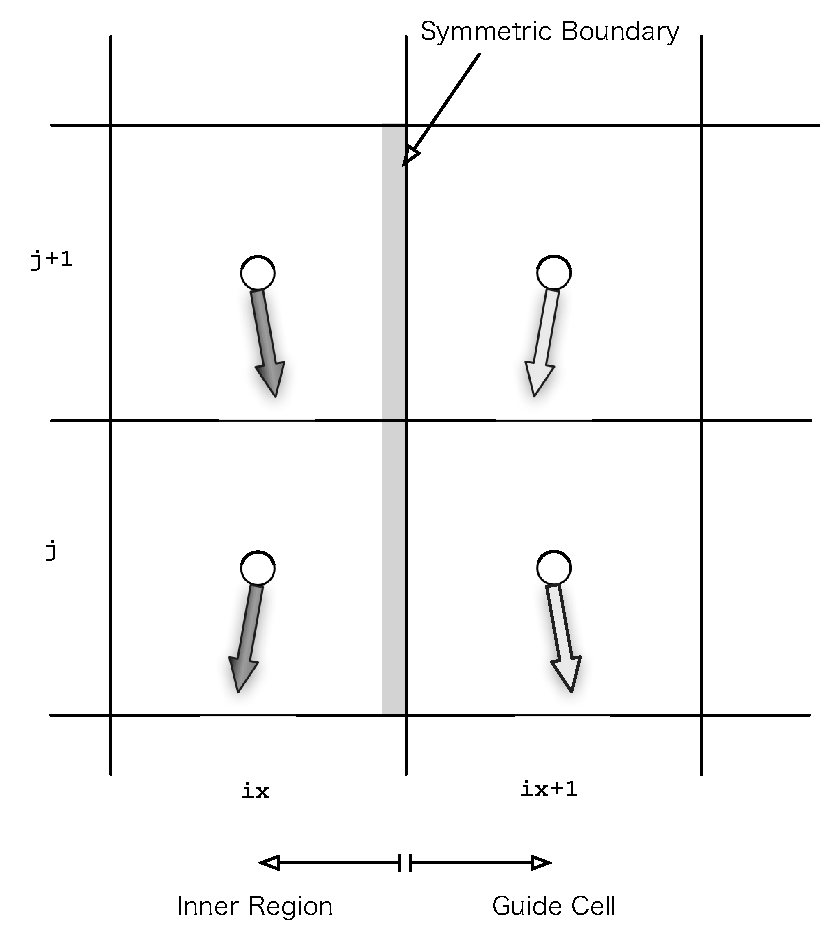
\includegraphics[width=7cm,clip]{symmetric.eps}
\end{center}
\caption{対称境界面における境界条件}
\label{fig:symmetric plane}
\end{figure}

熱計算では,対称境界が指定された面は断熱境界となります.


%%%
\pagebreak
\subsection{流出境界}

流出境界を指定する場合には,流出方向は既知とします.
外部境界では\textbf{図\ref{fig:outflow BC outer}}に示すようにガイドセルのセル属性は流体であることが必要です.
ガイドセルのセル属性の指定方法については\hyperlink{tgt:outer_boundary}{OuterBoundary}を参照してください.

{\small
\begin{program}
<OuterBoundary>
  <Elem name="Basic_BCs">
    <Elem name="outflow" id="3">
      <Param name="velocity_type" dtype="STRING" value="minmax" />
    </Elem>
  </Elem>
</OuterBoundary>
\end{program}
}

\begin{figure}[htbp]
\begin{center}
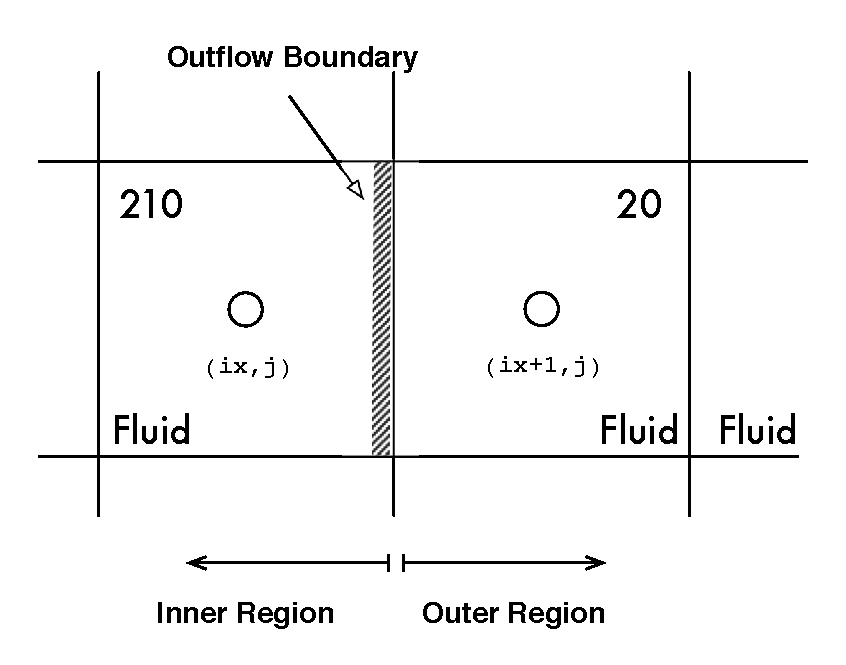
\includegraphics[width=8cm,clip]{outflowBC_outer.eps}
\end{center}
\caption{外部境界面における流出境界.x+方向の例.}
\label{fig:outflow BC outer}
\end{figure}

\noindent 指定するパラメータとして,境界条件番号と対流流出速度の評価方法があります.この例では,流出速度の評価方法にMinmaxを指定しています.
流出速度の選び方として,流出断面の平均速度や最大値と最小値の算術平均などが提案されており,経験上,内部流の場合にはAverageが流出速度のよい近似値を与えます.
一方,外部流や噴流のような無限空間の境界面の場合にはMinMaxがよい近似値となります.
流出速度の指定は,\textbf{表\ref{tbl:outflow velocity}}のようにVelocity\_TypeタグにてAverage または Minmaxを指定します.
Averageは,物体でブロックされていない有効セルの平均値をとります.
Minmaxは,境界面における有効セルの流速の最大値と最小値の算術平均値を与えます.

\begin{table}[htdp]
\caption{対流流出速度の評価方法の指定}
\begin{center}
\small
\begin{tabular}{ll} \toprule
Velocity\_Type & パラメータの説明\\ \midrule
Average & 流出面の有効セルに対する平均値\\
Minmax & 流出面の有効セルに対する最大値と最小値の算術平均値\\ \bottomrule
\end{tabular}
\end{center}
\label{tbl:outflow velocity}
\end{table}

圧力境界条件としては,Fractional Step法のアルゴリズムに適合するように,境界面上で$\nabla p=0$を用いています.

熱境界としても,速度と同様に,対流流出型の境界条件となります.



%%
\pagebreak
\subsection{速度指定境界}

この境界条件は,セル界面における運動量流束の形で実装されています.
まず,速度指定境界のXMLパラメータについて説明します.

{\small
\begin{program}
<OuterBoundary>
  <Elem name="Basic_BCs">
    <Elem name="Specified_Velocity" id="4">
      <Param name="Normal_x"        dtype="REAL"   value="0.0" />
      <Param name="Normal_y"        dtype="REAL"   value="1.0" />
      <Param name="Normal_z"        dtype="REAL"   value="0.0" />
      <param name="Profile"         dtype="string" value="Harmonic" />
      <param name="Specified_Type"  dtype="string" value="Velocity" />
      <Param name="Specified_Value" dtype="REAL"   value="7.0" />
      <Param name="Frequency"       dtype="REAL"   value="2.0" />
      <Param name="Initial_Phase"   dtype="REAL"   value="0.0" />
      <Param name="Constant_Bias"   dtype="REAL"   value="0.0" />
      <Param name="Temperature"     dtype="REAL"   value="20.0" />
    </Elem>
  </Elem>
</OuterBoundary>
\end{program}
}

\noindent 境界面の指定方法は,\textbf{表\ref{tbl:vspec parameter with heat}}に示すパラメータを与えます.
時間変化を伴う速度指定はProfile=\lq\lq Harmonic\rq\rq を指定し,\textbf{式(\ref{eq:harmonic out})}の形式の単振動の境界条件を周期や初期位相,固定バイアスと供に与えます.時間的に変化しない壁面境界の場合にはProfile=\lq\lq Constant\rq\rq を指定し,周波数,初期位相,固定バイアス値の指定は不要です.

圧力の境界条件は,壁面境界条件と同様にNeumann型の圧力境界条件$\nabla p=0$が用いられます.

温度の指定単位は,Unitセクションの\hyperlink{tgt:unit}{Temperature}で指定した単位になります.

\begin{table}[htdp]
\caption{速度指定境界のパラメータ}
\begin{center}
\small
\begin{tabular}{lll} \toprule
タグ & 指定キーワード & パラメータの説明\\ \midrule
Normal\_x & | & 法線ベクトルのx方向成分\quad 法線は単位ベクトル\\
Normal\_y & | & 法線ベクトルのy方向成分\\
Normal\_z & | & 法線ベクトルのz方向成分\\
Profile & Constant $|$ Harmonic & 指定速度のタイプ\\
Specified\_Type & Velocity & 指定単位 $[m/s]$\\
Specified\_Value & | & 速度\\
Frequency & | & 周波数 $f\, [Hz]$\\
Initial\_Phase & | & 初期位相 $\phi\, [Rad]$\\
Constant\_Bias & | & 一定値 $b\, [m/s]$\\
Temperature & | & 指定温度 $[K\,|\,{}^\circ\mathrm{C}]$\\
\bottomrule
\end{tabular}
\end{center}
\label{tbl:vspec parameter with heat}
\end{table}


%%
\pagebreak
\hypertarget{tgt:preriodic}{\subsection{周期境界}}

周期境界条件には,外部境界に対する周期境界と計算内部領域に設定する部分的な周期境界条件を併用する条件の2とおりがあります.
外部境界に対する周期境界条件では,\textbf{図\ref{fig:index_domain}}において,Inner\,Regionの両端の境界が重なる状態を想定しています.

\vspace{2mm}

外部境界に対する周期境界条件には\textbf{表\ref{tbl:periodic mode}}に示す3つのモードが指定できます.
下記には,各モードの例を示します.
Simple\_Copyモードは,周期境界条件面の両端で,単純に計算内部領域の値を他方のガイドセルにコピーします.
Pressure\_Diffrenceモードは,両端で圧力差を与える周期境界条件で,速度や温度についてはSimple\_Copyモードと同じですが,圧力は指定の圧力差を与えます.上流側と下流側の設定が必要です.
Driverモードは,乱流計算などで発達したチャネル流を上流境界として与えるためのしくみで,内部境界条件との組み合わせで利用します.Driverモードの説明は内部境界条件をご覧ください.

{\small
\begin{program}
<OuterBoundary>
  <Elem name="Basic_BCs">
    <Elem name="periodic" id="7" >
      <Param name="mode" dtype="string" value="Simple_Copy" />
    </Elem>
      
    <Elem name="periodic" id="8" >
      <Param name="mode"                dtype="string" value="Directional" />
      <Param name="flow_direction"      dtype="string" value="upstream" />
      <Param name="pressure_difference" dtype="REAL"   value="8.148e-3" />
    </Elem>
      
    <Elem name="periodic" id="9" >
      <Param name="mode"                dtype="string" value="Directional" />
      <Param name="flow_direction"      dtype="string" value="downstream" />
      <Param name="pressure_difference" dtype="REAL"   value="8.148e-3" />
    </Elem>
      
    <Elem name="periodic" id="10" >
      <Param name="mode"             dtype="string" value="driver" />
      <Param name="driver_direction" dtype="string" value="x_minus" />
    </Elem>
  </Elem>
</OuterBoundary>
\end{program}
}

\begin{table}[htdp]
\caption{周期境界条件のモード}
\begin{center}
\small
\begin{tabular}{ll} \toprule
キーワード & モードの説明\\ \midrule
Simple\_Copy & 周期境界の両端で物理量をガイドセルにコピーします.\\
Directional  & 圧力差を与える周期境界条件で,上流と下流の境界面を指定します.\\
Driver       & 計算領域内で部分的な周期境界条件を設定します.\\ \bottomrule
\end{tabular}
\end{center}
\label{tbl:periodic mode}
\end{table}

Directionalモードでは,\textbf{表\ref{tbl:parameter dir. mode}}に示すパラメータが必要で,Pressure\_Differenceの値が,UpstreamとDownstreamで同じ値である必要があります.

\begin{table}[htdp]
\caption{Directionalモードに必要なパラメータ}
\begin{center}
\small
\begin{tabular}{ll} \toprule
必要なキーワード & パラメータの説明\\ \midrule
Pressure\_Difference & 両端にかける圧力差 $[Pa]$\\
Flow\_Direction & Upstream(上流面)または Downstream(下流面)\\
\bottomrule
\end{tabular}
\end{center}
\label{tbl:parameter dir. mode}
\end{table}



%%%
\pagebreak
\subsection{遠方境界}

遠方境界条件として,トラクションフリー条件を用います.

\vspace{2mm}

トラクションフリー条件は,外部境界に対してのみ指定できる境界条件で,計算対象の主領域から遠方の挙動を仮定した条件です.
つまり,圧力の遠方条件$p=0$(基準圧)を考慮し,計算外部境界において流体の内部応力の法線方向成分がゼロである仮定を用いています.
この境界条件は,噴流のエントレインメントの効果などを考慮できる利点がありますが,渦が流出するような境界には適用できません.

次の例では,境界条件ID=4に遠方境界条件を設定しています.

{\small
\begin{program}
<OuterBoundary>
  <Elem name="Basic_BCs">
    <Elem name="traction_free" id="4">
      <Param name="Ambient_Temperature" dtype="REAL" value="25.0" />
    </Elem>
  </Elem>
</OuterBoundary>
\end{program}
}

熱流れの場合には,遠方場における温度を指定します.



%%%
\pagebreak
\subsection{流入出境界}

振動流のための特殊な境界条件で,実験的な境界条件です.

\vspace{2mm}

指定された外部境界面において,外部境界面の流速の符号に応じて流出境界と遠方条件を切り替えます.
下記の例では,流出境界条件に切り替わった場合の対流流出速度のパラメータをMinmaxに指定しています.

{\small
\begin{program}
<OuterBoundary>
  <Elem name="in_out" id="5">
    <Param name="velocity_type" dtype="STRING" value="minmax" />
    <Param name="Ambient_Temperature" dtype="REAL" value="25.0" />
  </Elem>
</OuterBoundary>
\end{program}
}

熱流れの場合には,流入時に対応する温度を指定します.



%%%-------------------------------------------------
\pagebreak
\section{内部境界条件}
内部領域の境界条件は,コンポーネントとして実装しています.
内部境界条件の多くは,計算空間内に局所的に存在し,複雑な計算処理を行います.
コンポーネントはそれらを効率よく取り扱うための機能です.
1つのセルを構成する6つの面にはそれぞれ別の境界条件を指定できますが,同種の流出境界は一つだけしか設定できません.

%
\subsection{壁面境界}

\subsubsection{流れの境界条件}
計算領域内部の壁面境界条件は,ボクセルモデルで固体壁に指定したセルIDが固体として認識され,セル界面の流束が指定する壁面速度から直接計算されるので,特に明示的な指定はありません.

壁面境界に対する圧力の境界条件は,Navier-Stokes方程式からNeumann型の圧力境界条件が得られます.
高レイノルズ数流れにおいては,粘性項の寄与が小さいと仮定し粘性項を省略し$\nabla p=0$の形式になります.
Binary近似の場合には,固体壁面との界面で$\nabla p=0$を満たすようにスキームが構成されています.

%
\subsubsection{熱境界条件}
壁面に対する熱境界条件としては,断熱,熱流束,熱伝達,等温,温度条件を指定できます.
熱境界条件の実装の詳細は\verb|Inside_CBC.pdf|をご覧ください.

%
\hypertarget{tgt:spec of heat bc}{\paragraph{熱境界条件の指定方法}}
熱境界条件は,セルの界面に与えます.多くの場合は流体と固体の界面ですが,固体熱伝導と共役熱移動の場合には,固体-固体界面の場合もあります.
内部境界の場合の界面の指定方法としては,指定する2つのIDで挟まれるボクセルの構成面を指定界面とします.
指定するIDの一つはキーIDで,主に固体セルを指定します.もうひとつのIDはDef\_Face IDです.

熱境界条件をコンポーネントとして与える場合,固体面をキーIDに指定します.
このときの熱流束の方向は,
\textbf{図\ref{fig:heat bc on solid}}において,固体面から流体側へ向かう法線をと同じ方向です.
つまり,この法線方向が指定する値の正の方向とし,流体側への熱移動を正の方向と考えます.

\begin{figure}[htbp]
\begin{center}
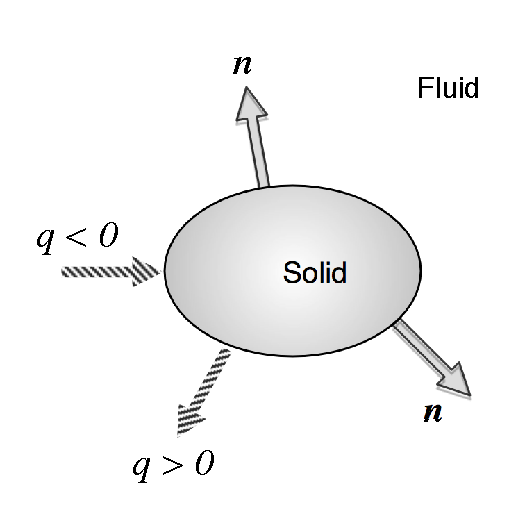
\includegraphics[width=6cm,clip]{heatBC.eps}
\end{center}
\caption{流体-固体界面における熱境界条件の熱流束の方向}
\label{fig:heat bc on solid}
\end{figure}

CBCの熱流体解析には幾つかのモードがあります.\hyperlink{tgt:solver_property}{Kind\_of\_Solver}の指定モードによって,計算空間内の計算対象とする部分が異なります.
Thermal\_FlowとThermal\_Flow\_Naturalの場合は,熱流動計算で流体の温度のみを解きます\footnote{計算の実装上,固体部分も解いていますが,その値はマスクされ,無効化されています.}.したがって,固体部分は計算対象とはならず不活性セルとして扱います.これより,流体-固体の境界面で与える熱境界条件(熱流束)は,流体セル側のみに指定されます.

一方,Solid\_Conductionの場合は,固体部分の熱伝導のみを解くので,流体部分を不活性セルとして扱います.したがって,流体-固体の境界面で与える熱境界条件は,固体セル側のみに指定されます.

Conjugate\_Heat\_Transferの場合には,流体と固体の両方の熱移動を計算します.したがって,流体-固体の境界面で与える熱境界条件は,流体セルと固体セルの両方で指定されます.

以下の各境界条件の指定で述べるように,IDとDef\_Faceタグの組み合わせにより,流体-固体の境界面を指定します.
このとき,\textbf{IDには固体のIDを,Def\_Faceには流体または固体のIDを指定すること}を基本としてください\footnote{IDに固体を指定する理由は,参照範囲を小さく抑えて効率的な計算をするためです.}.

%
\paragraph{断熱境界}
断熱壁では指定面で熱流束がゼロ,つまり$q^{\prime}=0$を指定します.固体セルと流体セルの界面に何も熱境界条件を指定しなければ,断熱境界条件となります.また,明示的に次のように\lq\lq Adiabatic\rq\rq セクションで断熱面を指定することができます.

{\small
\begin{program}
<InnerBoundary>
  <Elem name="Adiabatic" ID="6" comment="shield">
    <Param name="Def_Face" dtype="INT" value="3"/>
  </Elem>
</InnerBoundary>
\end{program}
}
この例では,ID=\lq\lq 6\rq\rq の固体セルのうち,ID=\lq\lq 3\rq\rq の流体セルに接する面に対して,断熱境界条件を指定しています.

%
\paragraph{熱流束境界}
熱流束境界は境界面で指定の熱流束を与えます.

{\small
\begin{program}
<InnerBoundary>
  <Elem name="Direct_Heat_Flux" ID="6" comment="outer_wall">
    <Param name="Def_Face"    dtype="INT"    value="3"/>
    <Param name="Heat_Flux"   dtype="REAL"   value="10.0"/>
  </Elem>
</InnerBoundary>
\end{program}
}

%
\paragraph{熱伝達境界}
熱伝達境界は次式の形式で熱流束を与える条件で,幾つかの種類があります.固体-流体セル間の熱伝達境界の与え方は,\hyperlink{tgt:heat-transfer}{外部境界条件の熱伝達境界}で説明した内容と同じです.

\begin{indentation}{3zw}{0zw}
%
\subparagraph{Type\_S  表面温度と熱伝達係数により計算}
Type\_Sは固体表面温度と熱伝達係数を与え,熱流束を計算します.
\textbf{式(\ref{eq:ht form})}において,$\theta_{\infty}^{\prime}$を固体表面に接する流体セルの値と仮定します.
以下に,熱境界部分のみパラメータ指定の一例を示します.

{\small
\begin{program}
<InnerBoundary>
  <Elem name="HeatTransfer_S" ID="6" comment="engine">
    <Param name="Def_Face"              dtype="INT"  value="3"/>
    <Param name="Surface_Temperature"   dtype="REAL" value="300.0"/>
    <Param name="Coef_of_Heat_Transfer" dtype="REAL" value="20.0"/>
  </Elem>
</InnerBoundary>
\end{program}
}

%
\subparagraph{Type\_SN  自然対流の乱流熱伝達}
自然対流の場合の乱流熱伝達の実験式を実装した境界条件です.

{\small
\begin{program}
<InnerBoundary>
  <Elem name="HeatTransfer_SN" ID="6" comment="engine">
    <Param name="Def_Face"                 dtype="INT"    value="3"/>
    <Param name="Surface_Temperature"      dtype="REAL"   value="500.0"/>
    <Param name="Ref_Temp_Mode"            dtype="STRING" value="Bulk_Temperature"/>
    <Param name="vertical_laminar_alpha"   dtype="REAL"   value="0.59"/>
    <Param name="vertical_laminar_beta"    dtype="REAL"   value="0.25"/>
    <Param name="vertical_turbulent_alpha" dtype="REAL"   value="0.1"/>
    <Param name="vertical_turbulent_beta"  dtype="REAL"   value="0.3333333"/>
    <Param name="vertical_ra_critial"      dtype="REAL"   value="1.0e9"/>
    <Param name="lower_laminar_alpha"      dtype="REAL"   value="0.27"/>
    <Param name="lower_laminar_beta"       dtype="REAL"   value="0.25"/>
    <Param name="lower_turbulent_alpha"    dtype="REAL"   value="0.27"/>
    <Param name="lower_turbulent_beta"     dtype="REAL"   value="0.25"/>
    <Param name="lower_ra_critial"         dtype="REAL"   value="1.0e9"/>
  </Elem>
</InnerBoundary>
\end{program}
}

%
\subparagraph{Type\_SF  強制対流の層流・乱流熱伝達}
強制対流の場合の層流・乱流熱伝達の実験式を実装した境界条件です.

{\small
\begin{program}
<InnerBoundary>
  <Elem name="HeatTransfer_SF" ID="6" comment="engine">
    <Param name="Def_Face"            dtype="INT"    value="3"/>
    <Param name="Surface_Temperature" dtype="REAL"   value="500.0"/>
    <Param name="Ref_Temp_Mode"       dtype="STRING" value="Bulk_Temperature"/>
    <Param name="alpha"               dtype="REAL"   value="0.037"/>
    <Param name="beta"                dtype="REAL"   value="0.8"/>
    <Param name="gamma"               dtype="REAL"   value="0.333333"/>
  </Elem>
</InnerBoundary>
\end{program}
}

%
\subparagraph{Type\_B  固体壁からの放熱条件}
熱伝達係数とバルク温度を与え,熱流束を計算します.固体熱伝導を解く場合の境界条件として利用します.

{\small
\begin{program}
<InnerBoundary>
  <Elem name="HeatTransfer_B" ID="6" comment="engine">
    <Param name="Def_Face"              dtype="INT"    value="3"/>
    <Param name="Bulk_Temperature"      dtype="REAL"   value="500.0"/>
    <Param name="Coef_of_Heat_Transfer" dtype="REAL"   value="0.12"/>
  </Elem>
</InnerBoundary>
\end{program}
}

\end{indentation}


%
\paragraph{等温壁境界}
等温壁境界は,指定面で温度が一定となる境界条件で,面温度を一定に保つような熱流束が発生します.

{\small
\begin{program}
<InnerBoundary>
  <Elem name="IsoThermal" ID="6" comment="outer_wall">
    <Param name="Def_Face"    dtype="INT"    value="3"/>
    <Param name="Temperature" dtype="REAL"   value="100.0"/>
  </Elem>
</InnerBoundary>
\end{program}
}


%%
\subsection{流出境界条件}

\paragraph{流れの境界条件}
計算領域内部に設定する流出境界について説明します.
\textbf{内部境界の場合には流出側のセルは固体セルであり,かつ流出方向に2セル必要になること}に注意してください.
つまり,\textbf{図\ref{fig:outflow BC inner}}においては,セル$(i,\,j)$は流体,セル$(i+1,\,j)$は固体を指定します.
ハッチング部分,つまり$(i,\,j)$セルの固体セルに隣接する面が流出境界として指定されています.
計算内部領域における境界面は,次のように対象となる面をid=20とid=210の2つのIDで挟むことにより指定します.
速度の流出面における対流速度の評価方法として流出コンポーネントの平均速度を用い,流出面における圧力境界は圧力勾配ゼロとしています.

{\small
\begin{program}
<InnerBoundary> 
  <Elem name="outflow" id="20" comment="out">
    <Param name="def_face"    dtype="INT"    value="210" />
  </Elem>
</InnerBoundary>
\end{program}
}

\begin{figure}[htbp]
\begin{center}
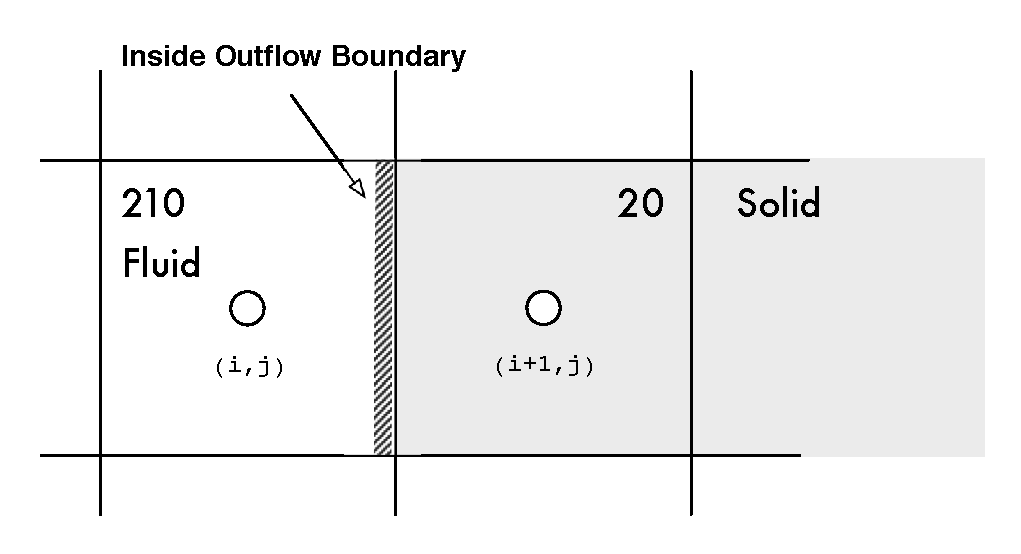
\includegraphics[width=8cm,clip]{outflowBC_inner.eps}
\end{center}
\caption{計算内部領域における流出境界の設定}
\label{fig:outflow BC inner}
\end{figure}

%
\paragraph{熱流出境界}
熱の流出境界は,流出界面の対流熱流束$\tilde{f}$を一次風上の形式で評価します.

\begin{equation}
\tilde{f} \,=\, \frac{\partial}{\partial x^{\prime}}\, \left( u^{\prime}\,\theta^{\prime} \right)_{upstream\_face}
\label{eq:outflow heat flux}
\end{equation}

分離解法において温度輸送方程式を解く過程では,速度は既知なので上式は直ちに計算できます.


%%%
\subsection{速度指定条件}

\paragraph{流れの境界条件}
この境界条件は,セル界面の運動量流束の形で実装されています.
まず,計算内部領域における流入境界のXML入力パラメータについて説明します.

{\small
\begin{program}
<InnerBoundary> 
  <Elem name="specified_velocity" id="3" comment="inlet">
    <Param name="Normal_x"        dtype="REAL"   value="0.0" />
    <Param name="Normal_y"        dtype="REAL"   value="0.0" />
    <Param name="Normal_z"        dtype="REAL"   value="-1.0" />
    <Param name="def_face"        dtype="INT"    value="6" />
    <param name="Profile"         dtype="string" value="Harmonic" />
    <param name="Specified_Type"  dtype="string" value="Velocity" />
    <Param name="Specified_Value" dtype="REAL"   value="7.0" />
    <Param name="Frequency"       dtype="REAL"   value="2.0" />
    <Param name="Initial_Phase"   dtype="REAL"   value="0.0" />
    <Param name="Constant_Bias"   dtype="REAL"   value="0.0" />
    <Param name="Temperature"     dtype="REAL"   value="50.0" />
  </Elem>
</InnerBoundary>
\end{program}
}

\noindent 境界面の指定方法は\textbf{表\ref{tbl:spec_vel}}に示すパラメータを与えます.
時間変化を伴う速度指定はProfile=\lq\lq Harmonic\rq\rq を指定し,\textbf{式(\ref{eq:harmonic_inner})}の形式の単振動\index{たんしんどう@単振動}の境界条件を周期や初期位相,固定バイアスと供に与えます.時間的に変化しない壁面境界の場合にはProfile=\lq\lq Constant\rq\rq を指定し,周波数,初期位相,固定バイアス値の指定は不要です.

\begin{equation}
V \,{=}\, A \sin \left( 2 \mathrm{\pi} ft \,+\, \phi \right) \,+\, b
\label{eq:harmonic_inner}
\end{equation}

\begin{table}[htdp]
\caption{コンポーネントの流束指定のパラメータ}
\begin{center}
\small
\begin{tabular}{ll} \toprule
キーワード & パラメータの説明\\ \midrule
Normal\_x & 法線ベクトルのx方向成分\quad 法線は単位ベクトル\\
Normal\_y & 法線ベクトルのy方向成分\quad 法線は単位ベクトル\\
Normal\_z & 法線ベクトルのz方向成分\quad 法線は単位ベクトル\\
Def\_Face & 指定面を特定する相手先のセルID\\
Profile & 指定速度のタイプ (Constant $|$ Harmonic)\\
Specified\_Type & 指定速度の単位 (Velocity $|$ Massflow)\\
Specified\_Value & 速度$A\, [m/s]$ または 流量$[m^3/sec.]$\\ 
Frequency & 周波数 $f\, [Hz]$\\
Initial\_Phase & 初期位相 $\phi\, [Rad]$\\
Constant\_Bias & 一定値 $b\, [m/s]$ または $[m^3/sec.]$\\
Temperature & 熱計算の場合に流入温度$[K\,|\,{}^\circ\mathrm{C}]$を指定\\
\bottomrule
\end{tabular}
\end{center}
\label{tbl:spec_vel}
\end{table}

\paragraph{熱境界条件}
指定面での対流熱流束を\textbf{式(\ref{eq:outflow heat flux})}で評価します.


%%%
\subsection{周期境界条件}
内部周期境界条件は外部の周期境界条件と組み合わせて利用します.
このため,外部境界条件指定で,次の指定が必要です.

{\small
\begin{program}
<OuterBoundary>
  <Elem name="Basic_BCs">
    <Elem name="periodic" id="10" >
      <Param name="mode"             dtype="string" value="driver" />
      <Param name="driver_direction" dtype="string" value="x_minus" />
    </Elem>
  </Elem>
</OuterBoundary>
\end{program}
}

\begin{table}[htdp]
\caption{Driverモードのパラメータ}
\begin{center}
\small
\begin{tabular}{ll} \toprule
必要なキーワード \\ \midrule
Driver\_Direction & X\_minus$\,|\,$X\_plus$\,|\,$Y\_minus$\,|\,$Y\_plus$\,|\,$Z\_minus$\,|\,$Z\_plus\\ \bottomrule
\end{tabular}
\end{center}
\label{tbl:parameter driver mode}
\end{table}

\paragraph{流れの境界条件}
内部の周期境界条件は,計算外部と計算領域内で部分的な周期境界条件を設定します.
モードとしてDriverを指定した場合には,下記のように同時に内部周期境界を指定しなければなりません.
Upstream\_DirectionとOuterBoundaryで指定するDriver\_Directionの方向は一致する必要があります.

{\small
\begin{program}
<InnerBoundary>
  <Elem name="periodic" id="4" comment="inner_driver" >
    <Param name="upstream_direction"  dtype="string" value="x_minus" />
    <Param name="pressure_difference" dtype="REAL"   value="1.636e-4" />
  </Elem>
</InnerBoundary>
\end{program}
}

現時点では,逐次計算しかできません.

\paragraph{熱境界条件}
熱境界に対しては,指定するパラメータはありません.


%%%
\subsection{セルボリュームに対する熱境界条件}
セル体積要素に作用するコンポーネントの熱境界条件を説明します.
この境界条件は,全てのセルに対して適用可能です.

\subsubsection{Specified\_Temperature}

以下の形式で指定温度を与えます.
{\small
\begin{program}
<InnerBoundary>
  <Elem name="Specified_Temperature" ID="60" comment="engine">
    <Param name="Temperature" dtype="REAL" value="45.0"/>
  </Elem>
</InnerBoundary>
\end{program}
}

\begin{table}[htdp]
\caption{温度指定のパラメータ}
\begin{center}
\small
\begin{tabular}{ll} \toprule
指定キーワード & パラメータの説明\\ \midrule
Temperature & 表面温度 $[K\,|\,{}^\circ\mathrm{C}]$\\
\bottomrule
\end{tabular}
\end{center}
\label{tbl:spec temp}
\end{table}

%
\subsubsection{Heat\_Generation}
\textbf{表\ref{tbl:heat_generation}}に示すように,発熱量または発熱密度を指定セルに与えることができます.
発熱量を指定した場合には,該当IDの体積を前処理で計算し,発熱密度に変換します.
次の例では,ID=60に10[$W$]の発熱量を与えています.

{\small
\begin{program}
<InnerBoundary>
  <Elem name="Heat_Source" ID="60" comment="heater">
    <Param name="Type"    dtype="STRING" value="Heat_Release_Value"/>
    <Param name="Value"   dtype="REAL"   value="10.0"/>
  </Elem>
</InnerBoundary>
\end{program}
}

\begin{table}[htdp]
\caption{発熱セルの指定方法}
\begin{center}
\small
\begin{tabular}{lll} \toprule
キーワード & パラメータの種類 & 単位\\ \midrule
Heat\_Release\_Value & 発熱量 & $[W]$\\
Heat\_Generation\_Density & 発熱密度 & $[W/m^3]$\\ \bottomrule
\end{tabular}
\end{center}
\label{tbl:heat_generation}
\end{table}


%%%
\hypertarget{tgt:inactive}{\subsection{不活性セル指定}}

計算空間内で,不活性化するセルIDを指定します.
コンポーネントの機能を使って実装しています.
\vspace{2mm}

不活性化の対象は,圧力と温度の計算に対してのみで,流体と固体の両方の属性をもつセルIDに適用できます.
不活性を指定されたセルは,圧力と温度の計算に関しては,意味のある計算をしません.代わりに,周囲のセルの平均値が代入されます.この処理はラプラス方程式を解くことに相当しますが,収束判定時にはその残差は考慮しません.下記のように,不活性化するセルIDを指定します.

{\small
\begin{program}
<InnerBoundary>
  <Elem name="Inactive" ID="600" comment="outer_layer"/>
</InnerBoundary>
\end{program}
}


%%%
\hypertarget{tgt:inactive}{\subsection{モニタ}}

計算空間内に設定する内部境界条件について,コンポーネント毎の積算値をモニターします.
下記の例では,ID=20で指定される領域をモニタ部とし,そこで速度,圧力をモニタすることを指定しています.
Normalはモニタ面の法線を指定しています.

{\small
\begin{program}
<InnerBoundary>
  <Elem name="Cell_Monitor" id="20" comment="monitor_inlet"> 
    <Param name="Normal_x" dtype="REAL" value="1.0" /> 
    <Param name="Normal_y" dtype="REAL" value="0.0" /> 
    <Param name="Normal_z" dtype="REAL" value="0.0" /> 
    <Elem name="Variables"> 
      <Param name="velocity"       dtype="STRING" value="on" /> 
      <Param name="pressure"       dtype="STRING" value="on" /> 
      <Param name="temperature"    dtype="STRING" value="off" /> 
      <Param name="Total_pressure" dtype="STRING" value="off" /> 
    </Elem> 
  </Elem>
</InnerBoundary>
\end{program}
}

指定方法の詳細は,\hyperlink{tgt:cell_monitor}{ボクセルモデルのセルIDで指定する方法}を参照してください.


%%
\hypertarget{tgt:external forcce}{\section{外力項を用いた境界条件}}

流動現象の中には空間スケールの異なる流れがあり相互に影響するような問題,例えば,多孔質層を通過する大空間の流れを解析する場合,興味の対象は大空間内の流動挙動であり,多孔質層内はマクロに見て適切な流れ場になっていればよいことも多くあります.
メッシュ解像度以下の微細な構造が流動特性に与える影響は,ダルシー則などのように理論的,あるいは実験式などで与えられます.
このような流体特性をもつ境界条件について説明します.

\subsection{圧力損失境界条件}
熱交換器やファンなどの圧力損失\index{あつりょくそんしつ@圧力損失}・利得をモデル化した境界条件について説明します.
熱交換器は,圧力損失を生じる多孔質物体として扱い,流出方向を法線で指定します.
この条件は,通過流量(流速)と圧力損失量の関係式が与えられるものとします.

一方,ファンは圧力利得が関係式として与えられます.
ファンの場合には旋回成分などもありますが,ここでは軸流方向のみを考えます.
このような流体部品のモデル指定は,セルボリュームに作用する内部境界条件として指定します.
具体的には,コンポーネント\index{コンポーネント}のPressure\_Lossとして扱い,\textbf{式(\ref{eq:ploss_NS})}の外力項$F_{i}$として実装します.
$\beta$はセル内部におけるコンポーネントの体積占有率\index{せんゆうりつ@占有率}(Volume Fraction; VF)\index{Volume Fraction}です.
外力項として,\textbf{表\ref{tbl:ploss_model}}のようなモデルが実装されています.

この境界条件に対応するモニタ量として,指定部の平均速度・流量や圧力損失量がhistory\_compo.logに書き出されます.
詳細は\hyperlink{tgt:history_compo}{コンポーネント履歴}を参照してください.

\begin{table}[htdp]
\caption{セルボリュームに作用する内部境界条件}
\begin{center}
\small
\begin{tabular}{ll} \toprule
キーワード & 境界条件モデル \\ \midrule
%Fan & ファンモデル  \\ 
Pressure\_Loss & 熱交換器モデル \\ 
%Darcy & 多孔質体に対するDarcyモデル & \\ 
\bottomrule
\end{tabular}
\end{center}
\label{tbl:ploss_model}
\end{table}

\begin{equation}
{\frac{\partial{u}_{i}}{\partial{t}}}^{{n}{+}{1}}{+}\,\frac{\partial}{\partial{x}_{j}}\left({{u}_{i}{u}_{j}}\right)
\,{=}\,
{-}{\frac{\partial{p}}{\partial{x}_{i}}}^{{n}{+}{1}}{+}\,{(}{1}{-}\mathrm{\beta}{)}\frac{\partial{\mathrm{\tau}}_{ij}}{\partial{x}_{j}}\,{+}\,\beta {F_{i}}^{n+1}
\label{eq:ploss_NS}
\end{equation}

%
\paragraph{熱交換器のモデル化}

圧力損失の一つである熱交換器モデルは,\textbf{式(\ref{eq:ploss_NS})}に\textbf{式(\ref{eq:ploss_force})}の実験式を適用します.
\begin{equation}
{F}_{i}
\,{=}\,
-sgn \left( u_{i} \right) {\left( \frac{\Delta p}{\Delta r} \right)}^{R} {n_{i}}^{R}
\label{eq:ploss_force}
\end{equation}

\noindent ここで,${}^{R}$は熱交換器を表し,$\Delta p,\,\Delta r,\,n_{i}$はそれぞれ圧力損失量,熱交換器の厚さ,法線方向を表します.
熱交換機の通過ベクトルとは逆方向に圧力損失が発生するモデルとなっています.
ただし,パラメータvectorがdirectionalでない場合には,速度ベクトルは熱交換器の流出方向には揃わず.単に,圧力損失が計算された速度ベクトルと逆向きに作用するモデルとなります.
圧力損失パラメータは,熱交換器の性能試験結果により,\textbf{図\ref{fig:ploss}}に示すような実験値が得られます.
$\Delta p-V$の性能線図を$[mmAq - m/s]$を単位とした場合のパラメータの取得について示します.
熱交換器の圧力損失は,二次多項式で近似できます.
\textbf{図\ref{fig:ploss}}のグラフの読みからカーブフィットを行い,\textbf{式(\ref{eq:dp-v})}に対応する数値$c_{1}$ -- $c_{4}$, $u_{threshold}$を得ます.ダッシュは有次元を表します.
このとき,圧力損失ヘッドの単位に応じて,パラメータは無次元量に変換されます.
\begin{equation}
{h}^{\prime}
\,{=}\,
\begin{cases}
\, c_{1} {u^{\prime}}^{2}\,+\,c_{2}u^{\prime}\,+\,c_{3} & \quad (u^{\prime} \geqq u^{\prime}_{threshold})\\
\, c_{4} {u^{\prime}}^{2} & \quad (u^{\prime}<u^{\prime}_{threshold})\\
\end{cases} \quad [mm]
\label{eq:dp-v}
\end{equation}

\begin{figure}[htdp]
\begin{center}
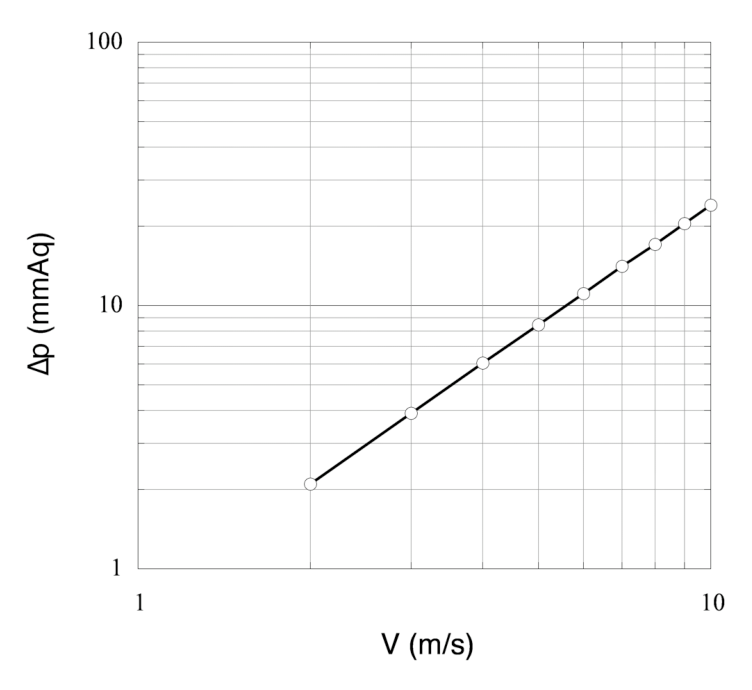
\includegraphics[width=10cm,clip]{ploss.eps}
\end{center}
\caption{$\Delta p-V$性能線図(対数表示)}
\label{fig:ploss}
\end{figure}

\begin{figure}[htdp]
\begin{center}
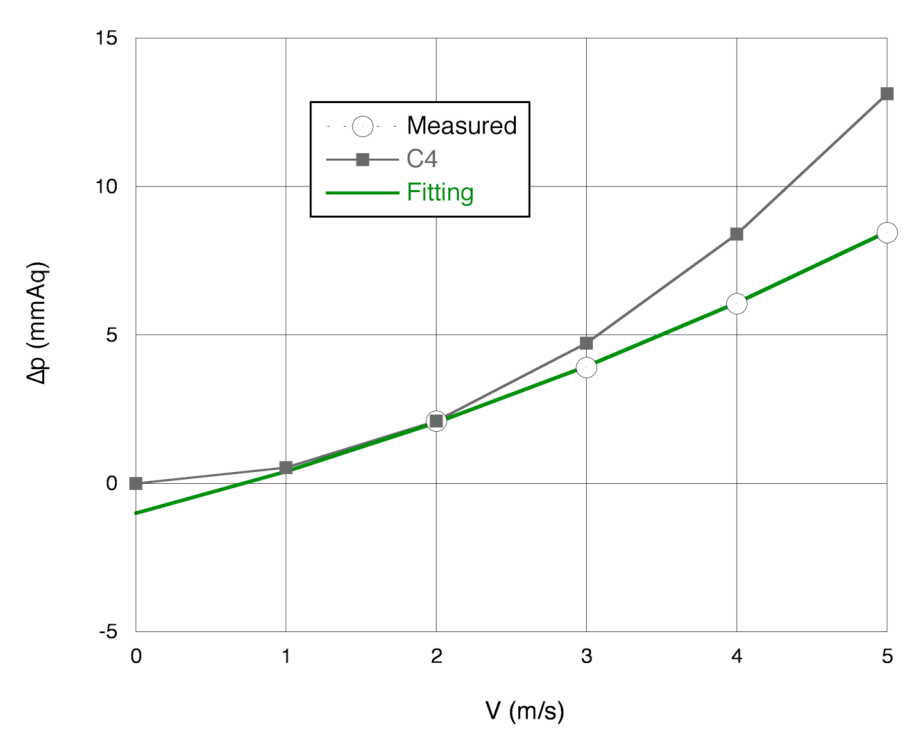
\includegraphics[width=10cm,clip]{rad_para.eps}
\caption{パラメータの取得(\textbf{図\ref{fig:ploss}}と同じものを線形表示)}
\label{fig:get_para}
\end{center}
\end{figure}

\textbf{図\ref{fig:get_para}}に計算パラメータの取得方法を示します.一般に,低速域のデータは得られない場合が多く,推定が必要です.
図では○が測定結果を示し2$[m/s]$より低速域のデータはありません.
そこで,測定値を元にカーブフィッティングを行い(図中の緑色の曲線),算出された係数$c_{1}=0.12321,\,c_{2}=1.2806,\,c_{3}=-1.0074\quad(2-10\,[m/s])$を計算パラメータとします.
この場合,$h'$切片がマイナスになるため,熱交換機の通過速度がゼロに近い場合に急にマイナスの圧力損失(つまり圧力利得)が発生し,実際の現象とは異なり計算上好ましくありません.
そこで\textbf{式(\ref{eq:dp-v})}に示すようにある閾値で曲線を切り替えます.
ここでは,測定された最小速度$u_{threshold}=2\,[m/s]$を閾値として,C4のカーブ$c_{4}=0.525\quad(0-2\,[m/s])$で切り替えます.
熱交換器厚さは実務での観点から単位を$[mm]$で指定するので,注意してください.\\

次の例では,境界条件番号8に圧力損失条件を設定します.
ここで各パラメータは\textbf{表\ref{tbl:ploss_table_ibc}}に対応します.

{\small
\begin{program}
<InnerBoundary>
  <Elem name="Pressure_Loss" ID="8" comment="radiator"/>
    <Param name="Unit"        dtype="STRING" value="mmAq"/>
    <Param name="Normal_x"    dtype="REAL"   value="1.0" />
    <Param name="Normal_y"    dtype="REAL"   value="0.0" />
    <Param name="Normal_z"    dtype="REAL"   value="0.0" />
    <Param name="c1"          dtype="REAL"   value="0.8" />
    <Param name="c2"          dtype="REAL"   value="0.0" />
    <Param name="c3"          dtype="REAL"   value="0.0" />
    <Param name="c4"          dtype="REAL"   value="0.8" />
    <Param name="u_threshold" dtype="REAL"   value="0.2" />
    <Param name="Thickness"   dtype="REAL"   value="80" />
    <Param name="Vector"      dtype="STRING" value="Directional" />
  </Elem>
</InnerBoundary>
\end{program}
}

\begin{table}[htdp]
\caption{圧力損失モデルのパラメータ}
\begin{center}
\small
\begin{tabular}{lll} \toprule
キーワード & パラメータの説明\\ \midrule
Normal\_x & 熱交換器の法線ベクトルのx方向成分\quad 法線は単位ベクトル\\
Normal\_y & 熱交換器の法線ベクトルのy方向成分\quad 法線は単位ベクトル\\
Normal\_z & 熱交換器の法線ベクトルのz方向成分\quad 法線は単位ベクトル\\
c1 & 熱交換器の圧力損失係数\,c1\quad $[mmAq\,|\,mmHg\,|\,Pa\,|\,Non dimension]$\\
c2 & 熱交換器の圧力損失係数\,c2\quad $[mmAq\,|\,mmHg\,|\,Pa\,|\,Non dimension]$\\
c3 & 熱交換器の圧力損失係数\,c3\quad $[mmAq\,|\,mmHg\,|\,Pa\,|\,Non dimension]$\\
c4 & 熱交換器の圧力損失係数\,c4\quad $[mmAq\,|\,mmHg\,|\,Pa\,|\,Non dimension]$\\
u\_threshold & 圧力損失カーブの切り替え速度 $u_{threshold}$ $[m/s\,|\,Non dimension]$\\
thickness & 熱交換器の厚さ\quad $[mm\,|\,Non dimension]$\\
unit & 圧力損失$\Delta p-V$線図のヘッドの単位\quad [$mmAq\,|\,mmHg\,|\,Pa\,|\,Non-Dimension]$ \footnotemark[4]\\
vector & 速度ベクトルの法線方向への強制\quad $[Directional \,|\, Non\_Directional]$\\  \bottomrule
\end{tabular}
\end{center}
\label{tbl:ploss_table_ibc}
\end{table}
\footnotetext[4]{mmAqは水(300K, p=101.325kPa)996.62 $[kg/m^3]$,mmHgは水銀(300K)13538 $[kg/m^3]$をプログラム中でハードコード.}


%%%
\begin{comment}

%
\paragraph{Fan}
\begin{indentation}{3zw}{0zw}
Fanモデル...
\end{indentation}

%
\paragraph{Darcy model}
\label{Darcy model param}
\begin{indentation}{3zw}{0zw}

\ref{sec:porous model}で説明したDarcyモデルでは,等方と非等方モデルが利用できる.透過率パラメータは,\textbf{表\ref{tbl:permeability parameter}}に示すように各主軸方向毎に与える.等方モデルの場合には,各方向のパラメータを同じ値にする.

{ \small
\begin{program}
<Elem name="Forcing_Volume" id="1">
  <Elem name="Darcy" id="50" comment="porous">
    <Param name="permeability_x"  dtype="REAL" value="2.0" />
    <Param name="permeability_y"  dtype="REAL" value="3.0" />
    <Param name="permeability_z"  dtype="REAL" value="4.0" />
  <\Elem>
<\Elem>
\end{program}
}

\begin{table}[htdp]
\caption{Darcyモデルのパラメータ}
\begin{center}
\small
\begin{tabular}{ll} \toprule
キーワード & パラメータの説明\\ \midrule
permeability\_x & x方向の透過率 $[m^2]$\\
permeability\_y & y方向の透過率 $[m^2]$\\
permeability\_z & z方向の透過率 $[m^2]$\\ \bottomrule
\end{tabular}
\end{center}
\label{tbl:permeability parameter}
\end{table}

\end{indentation}

\end{comment}
%%%




%%%
\section{静止座標系と移動座標系の場合の境界条件}
\label{sec:moving_grid}

外部流を考えます.
\textbf{図\ref{fig:reference_frame}}(a)の静止座標系\index{ざひょうけい@座標系!せいし@静止---}と\textbf{図\ref{fig:reference_frame}}(b)の移動座標系\index{ざひょうけい@座標系!いどう@移動---}のように異なる座標系で物体まわりの流れを計算する場合,境界条件の与え方が異なります.
静止座標系は風洞実験に相当し,静止した対象物に対して風をあてている状況です.テストセクション(この場合は計算領域)から出ていく流れが流出風に相当します.
一方,移動座標系では対象物に固定した計算格子が対象物とともに静止流体中を移動します.この場合は,計算領域そのものと内部の格子が物体とともに動きます.
一定速度$V$で動いている座標系の添え字を${}_M$とし,静止した座標系の添え字を${}_S$とします.
いま,静止座標系で観測される流体の速度を$u_{S}$と表すと,同じ速度は移動座標系では$u_{M}-V$のように観測されます.
つまり,
\begin{equation}
u_{S} \, = \, u_{M}-V
\label{eq:galilei}
\end{equation}

\begin{figure}[htbp]
\begin{center}
\subfigure[静止座標系]{
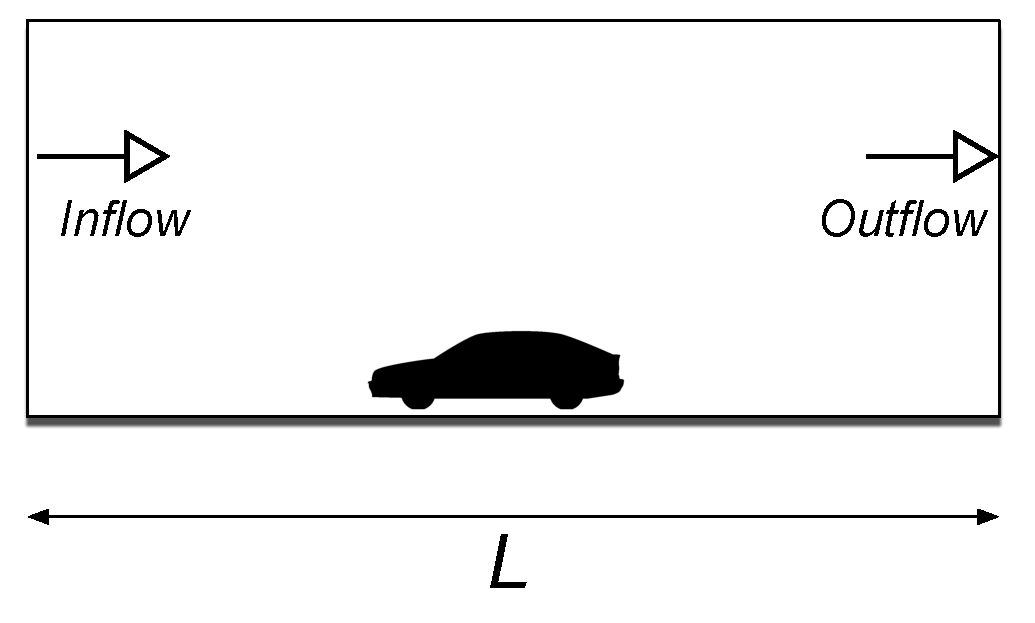
\includegraphics[width=8cm,clip]{stationary.eps}
}
~
\subfigure[移動座標系]{
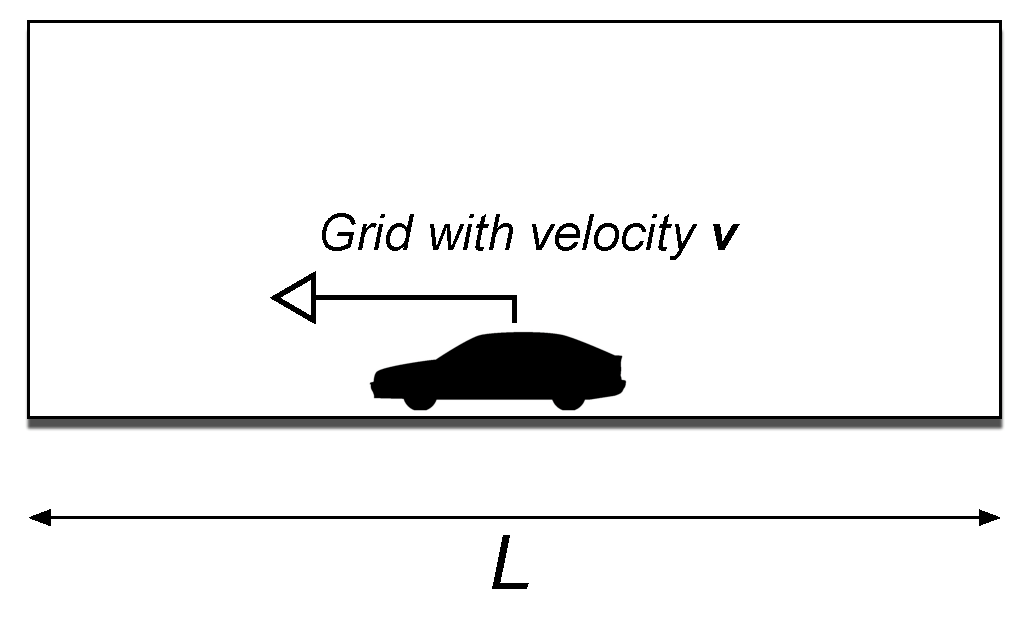
\includegraphics[width=8cm,clip]{moving.eps}
}
\caption{静止座標系と移動座標系の観測点の違い} 
\label{fig:reference_frame}
\end{center}
\end{figure}

静止座標系において\textbf{図\ref{fig:reference_frame}}(a)のような境界条件を与える場合,流入部では$u_{0}$を与えます.
一方,移動座標系では静止流体の条件,つまり$u=0,\,p=0$を想定し,格子速度$V=-u_{0}$を与えると両者は等価になります.

移動座標系の場合注意を要するのが,物体と地面の境界条件です.物体は移動しているので格子速度と同じになります.
一方,地面は静止している地面と動いている地面の二通りが考えられます.
前者は風洞実験で固定地面板に相当し,後者はムービングベルトに相当します.
ムービングベルトの場合には物体と格子速度だけ相対速度をもっていることになります.
したがって,

\begin{equation}
u_{ground}\,=\,
\begin{cases}
\, -u_{0} & \quad (Stationary\,ground)\\
\, 0 & \quad (Moving\,ground)\\
\end{cases}
\label{eq:relative velocity wall}
\end{equation}

移動格子の移動速度は\hyperlink{tgt:reference_frame}{Reference\_Frame}セクションで与えます.






%



%%%
\chapter{モニタリング機能}
\label{chpt:monitor}
\begin{abstract}
CBCソルバークラスには,計算中の任意点の物理量をモニターする仕組みがあります.本章では,その指定方法について説明します.
\end{abstract}
%
\graphicspath{{./fig_Monitor/}}


物理量モニタリング機能は,ユーザが指定した位置で指定した物理量をファイルに出力する機能です.
位置の指定には,XMLパラメータファイルで指定する方法とボクセルモデルのIDで指定する方法の2種類があります.


%%%
\section{XMLコンフィギュレーションファイルで指定する方法}
モニタリングの指定は,Monitor\_Listセクションに記述します.

{\small
\begin{program}
<Elem name="Monitor_List"> 
  <Param name="Log"                    dtype="STRING" value="On" />
  <Param name="output_mode"            dtype="string" value="Gather" />
  <Param name="Unit"                   dtype="STRING" value="Non_Dimensional" />
  <Param name="Sampling_Interval_Type" dtype="string" value="Time" />
  <Param name="Sampling_Interval"      dtype="real"   value="0.1" />
  
  <Elem name="point_set" comment="p1"> 
    <Param name="variable" dtype="string" value="velocity" /> 
    <Param name="variable" dtype="string" value="temperature" /> 
    <Param name="sampling_method" dtype="string" value="interpolation" /> 
    <Param name="sampling_mode"   dtype="string" value="all" /> 
    <Elem name="set" comment="10_Eng_ctr">
      <Param name="x" dtype="REAL" value="-0.217" /> 
      <Param name="y" dtype="REAL" value="-0.006" /> 
      <Param name="z" dtype="REAL" value="0.715" /> 
    </Elem> 
    <Elem name="set" comment="102_Eng_mnt_Rh_Fr"> 
      <Param name="x" dtype="REAL" value="-0.204" /> 
      <Param name="y" dtype="REAL" value="0.495" /> 
      <Param name="z" dtype="REAL" value="0.574" /> 
    </Elem> 
  </Elem> 

  <Elem name="line" comment="line_y=0"> 
    <Param name="variable" dtype="string" value="velocity" /> 
    <Param name="division" dtype="int" value="64" /> 
    <Param name="sampling_method" dtype="string" value="smoothing" /> 
    <Param name="sampling_mode"   dtype="string" value="fluid" /> 
    <Elem name="from"> 
      <Param name="x" dtype="REAL" value="0.0" /> 
      <Param name="y" dtype="REAL" value="0.0" /> 
      <Param name="z" dtype="REAL" value="-0.5" /> 
    </Elem> 
    <Elem name="to"> 
      <Param name="x" dtype="REAL" value="0.0" /> 
      <Param name="y" dtype="REAL" value="0.0" /> 
      <Param name="z" dtype="REAL" value="0.5" /> 
    </Elem> 
  </Elem> 
</Elem> 
\end{program}
}

\begin{table}[htdp]
\caption{モニター機能の設定}
\begin{center}
\small
\begin{tabular}{lll}\toprule
タグ & キーワード & 説明\\\midrule
Log & On $|$ Off & 機能の有効・無効\\
Output\_Mode & Gather $|$ Distribute & モニターログの出力モード\\
Unit & Dimensional $|$ Non\_Dimensional & 指定パラメータと出力ログの単位指定\\
Sampling\_Interval\_Type & Step $|$ Time & 間隔の指定形式\\
Sampling\_Interval & | & サンプリング間隔\\
\bottomrule
\end{tabular}
\end{center}
\label{tbl:outline of monitor}
\end{table}


Monitor\_Listには,点群(point\_set)と線分(line)の2種類の指定方法があります.
それぞれをグループと呼び,point\_setの構成点をsetと定義します.
ファイルへの出力はグループ毎に書き出されます.
XMLファイル中のpoint\_setまたはlineのパラメータのcommentは,
履歴ファイルの名前の末尾に追加されます.
各point\_set/lineタグのcommentは,履歴ファイル中で各モニタ点を識別する
ヘッダになり,ヘッダには座標も記述されます.
もし,setのcommentの記述がない場合には,
「point \#」(\#にはモニタ点番号)がヘッダとして与えられます. 

出力ファイルは\hyperlink{tgt:output_data}{OutputData}セクションで指定します.
出力モードは\hyperlink{tgt:monitor_list}{Monitor\_List}セクションのsampling\_outputタグで指定します.
出力モードは並列計算時のファイル出力様式で,
マスターノードに集約してファイル出力する場合にはgatherを指定し,
分散ノード毎にファイル出力する場合にはdistributeを指定します.
ファイル名の命名ルールは以下のようになっています.
\begin{itemize}
\item[-] 逐次実行時はOutputDataのlog\_samplingで指定されるファイル名
(例えば,history\_sampling.log)に,
グループ名(point\_setまたはlineのコメントで指定された文字列)を
追加したファイル名となります.
例えば,point\_setでp1がコメントとして与えられるグループに対しては,
history\_sampling\_p1.logというファイル名となります.
\item[-] 並列実行時,sampling\_output=gatherを指定した場合,
ファイル名は逐次と同じになります.
\item[-] 並列実行時,sampling\_output=distributeを指定した場合,
上記のファイル名に対して,更にランク番号を追加した ファイル名となります.
例えば,OutputDataのlog\_samplingでhistory\_sampling.logが指定され,
lineでline\_y=0がコメントとして与えられるグループに対しては,
history\_sampling\_line\_y=0.*.log となります(*にはランク番号が入ります). 
\end{itemize}

Pram name=\lq\lq variable\rq\rq で指定されるパラメータは,以下のキーワードによりモニタリングする物理量を指定します.

\begin{quote}
\begin{tabbing}
\hspace{8em}\= \hspace{20em}\kill
Velocity \>  速度\\
Pressure \> 圧力\\
Temperature \> 温度\\
Total\_Pressure \>  全圧\\
Vorticity \>  渦度
\end{tabbing}
\end{quote}
物理量はpoint\_setの例のように複数指定可能です.

Pram name=\lq\lq sampling\_method\rq\rq で指定されるパラメータは,以下のキーワードにより採取方法を指定します.
\begin{quote}
\begin{tabbing}
\hspace{8em}\= \hspace{20em}\kill
nearest \> モニタ点を含むセルでの値 \\
interpolation \> 三重線形補間\\
smoothing \> 局所平均による平滑化
\end{tabbing}
\end{quote}
Pram name=\lq\lq sampling\_mode\rq\rq で指定されるパラメータは,以下のキーワードにより採取モードを指定し,各採取方法での対象セルを指定します.
\begin{quote}
\begin{tabbing}
\hspace{8em}\= \hspace{20em}\kill
all \> 全セルを対象\\
fluid \> 流体セルのみを対象\\
solid \> 固体セルのみを対象
\end{tabbing}
\end{quote}

モニタリング指定された点はセルID=\lq\lq 255\rq\rq が割り当てられ,測定位置情報が書き込まれたsvx/sbxファイルが出力されます.

%%%
\subsection{値の採取方法}
\paragraph{nearest}
モニタ点を含むセルのセル中心での値を採取します.
nearestではSampling\_Mode=\lq\lq All\rq\rq に固定です.

\paragraph{interpolation}
モニタ点を囲む8つセル中心位置での値を採取し,
xyzの3方向に対して線形補間を行いモニタ点での値を評価します.
sampling\_mode=\lq\lq all\rq\rq の場合には,モニタ点を囲む8つセルの状態(流体/固体)によらず,常に三重線形補間を行います.
sampling\_mode=\lq\lq fluid\rq\rq の場合には,モニタ点を囲む8セル全てが流体セルの場合のみ三重線形補間を行い,それ以外の場合にはモニタ点を含むセル中心での値を採取します(nearest相当).
sampling\_mode=\lq\lq solid\rq\rq の場合も同様に,モニタ点を囲む8セル全てが固体セルの場合のみ三重線形補間を行い,それ以外の場合にはモニタ点を含むセル中心での値を採取します(nearest相当).

\paragraph{smoothing}
モニタ点を含むセルおよびその隣接セルでのセルセンタの値を採取して,その平均値(局所平均値)を計算します.
sampling\_mode=\lq\lq all\rq\rq の場合には,6つの全隣接セルを用いて,合計7セルでの値を採取して平均します.
sampling\_mode=\lq\lq fluid\rq\rq の場合には,モニタ点を含むセルと,そこに隣接する流体セルのみから平均値を計算します.
sampling\_mode=\lq\lq solid\rq\rq の場合には,モニタ点を含むセルと,そこに隣接する固体セルのみから平均値を計算します.

%%
\subsection{指定パラメータの制限およびエラー処理}
\begin{itemize}
\item[-] point\_setグループに所属するモニタ点に計算対象領域外の座標値があると,初期化時にエラーメッセージを出力してソルバーの実行を停止します.
\item[-] Lineグループで指定された線分は,必要なら計算対象領域内にクリッピングしてから,線分上の両端を含む分割点をモニタ点に定めます.
線分が完全に計算対象領域外にある場合には,エラーメッセージを出力してソルバーの実行を停止します.
このようなケースは\textbf{図\ref{fig:invalid_case}}に示すような場合が想定されます.
\item[-] 採取方法がinterpolationまたはsmoothingにおいて採取モードがfluidまたはsolidの場合には,次の条件を満たすモニタ点があると,ソルバー初期化時に警告メッセージが出力され,ソルバー実行中にはそのモニタ点での採取はスキップされます.
\begin{itemize}
\item[] sampling\_mode=\lq\lq fluid\rq\rq だが,モニタ点を含むセルが固体セルであった
\item[] sampling\_mode=\lq\lq solid\rq\rq だが,モニタ点を含むセルが流体セルであった
\end{itemize}
\end{itemize}

\begin{figure}[htbp]
\begin{center}
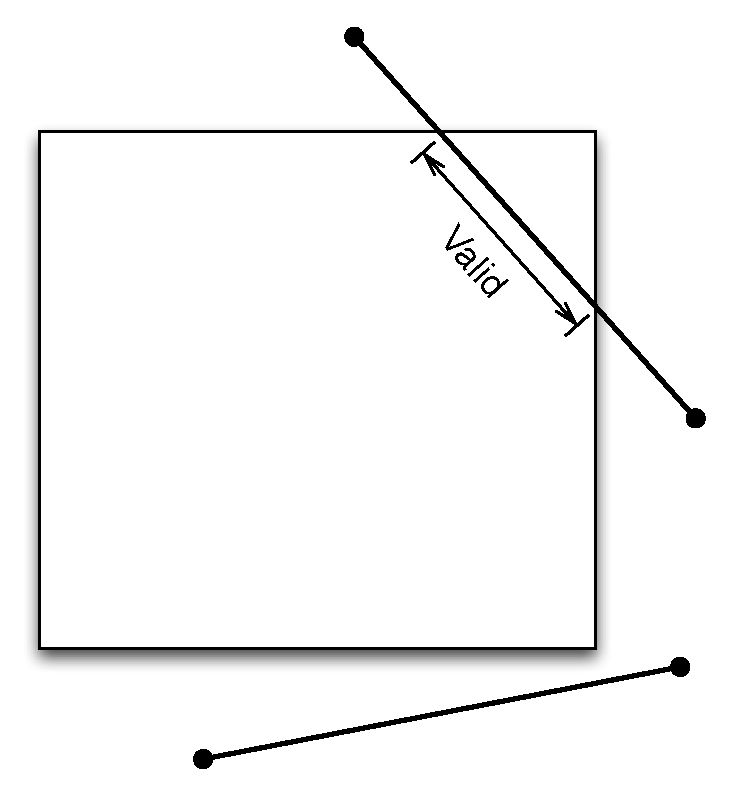
\includegraphics[width=6cm,clip]{Invalid_case.eps}
\end{center}
\caption{ラインのサンプリング指定で無効なケース}
\label{fig:invalid_case}
\end{figure}


%%
\subsection{出力ファイルフォーマット}
採取された物理量は,グループ毎にファイルに出力されます.
出力ファイルは,テキストファイルで,
モニタ点座標とモニタ変数を記述した{\bf ヘッダ領域}と,それに続く,
採取したステップ数個の{\bf データ領域}からなります.
ヘッダ領域とデータ領域,および,隣接するデータ領域間は1行の空行で区切られています.

\paragraph{ヘッダ領域}
1行目の整数nにモニタ点数と,モニタ対象の物理量を示すキーワード(Velocity, Presure等)が並びます.
続くn行に,各モニタ点の座標値およびcommentが出力されます.
なお,分散出力時には,nは担当ノード内のモニタ点数になり,担当モニタ点の座標値のみを出力します.
\begin{center}
\vspace{0.2\baselineskip}
\begin{tabular}{|p{14em}|p{20em}}\cline{1-1}
n Velocity Presure Temperature  & ← n点で速度,圧力,温度をモニタ\\ 
$x_1$  $y_1$  $z_1$  \#comment  & ← 各モニタ点の座標とcommentを\\
$x_2$  $y_2$  $z_2$  \#comment  &  空白区切りで出力\\
  …                   & \\
$x_n$ $y_n$ $z_n$    \#comment & \\
\cline{1-1}
\end{tabular}
\vspace{0.2\baselineskip}
\end{center}

\paragraph{データ領域}
1行目に,採取時のステップ数step(整数)とソルバー内部時間time(実数)が出力されます.
続くn行に,各モニタ点で採取した値が,ヘッダ領域のキーワードの並び順に出力されます.
\begin{center}
\vspace{0.2\baselineskip}
\begin{tabular}{|p{14em}|p{20em}}\cline{1-1}
step time  & ← ステップ数=step, 時間=time\\ 
$u_1$  $v_1$  $w_1$ $p_1$ $t_1$  & ← モニタ点毎の採取値が\\
$u_2$  $v_2$  $w_2$ $p_2$ $t_2$  &   空白区切りで並ぶ\\
  …                             &   ($u_i,v_i,w_i$)=速度,$p_i$=圧力,$t_i$=温度\\
$u_n$ $v_n$ $w_n$ $p_n$ $t_n$  & \\
\cline{1-1}
\end{tabular}
\vspace{0.2\baselineskip}
\end{center}

採取値の有効桁数は,単精度計算では小数点以下7桁,倍精度計算では16桁です.

なお,採取モードの制限により採取をスキップされたモニタ点では,データ領域の該当する行には,「*NA*」の文字列が出力されます.


%%%
\pagebreak
\hypertarget{tgt:cell_monitor}{\section{ボクセルモデルのセルIDで指定する方法}}
セルIDにより指定する方法は,各セル中心をモニタ点として,
sampling\_method=\lq\lq nearest\rq\rq , sampling\_mode=\lq\lq all\rq\rq の条件で採取を行います.

%
\subsection{モニター部の指定}
計算領域の内部において,物理量をモニタしたい部分をボクセルモデルのセルIDにより指定します.
モニタ面は基本的には,座標軸に面直な面とします.
ただし,若干予測精度は低下するが,軸に対して斜めの領域も指定できます.
condition.txt内のComponent Informationの部分にモニタ面の推定法線と面積の情報が表示されるので,確認してください.
ひとつのIDに対しては,単連結領域(一つの塊)となるようにIDを割り当てる必要があります.

\vspace{5mm}
\begin{indentation}{2zw}{0zw}

下記の例では,ID=20で指定される領域をモニタ部とし,そこで速度,圧力,全圧をモニタすることを指定しています.モニタ面の法線を指定しています.

{\small
\begin{program}
<InnerBoundary>
  <Elem name="Cell_Monitor" id="20" comment="monitor_inlet"> 
    <Param name="Normal_x" dtype="REAL" value="1.0" /> 
    <Param name="Normal_y" dtype="REAL" value="0.0" /> 
    <Param name="Normal_z" dtype="REAL" value="0.0" /> 
    <Elem name="Variables"> 
      <Param name="velocity"       dtype="STRING" value="on" /> 
      <Param name="pressure"       dtype="STRING" value="on" /> 
      <Param name="temperature"    dtype="STRING" value="off" /> 
      <Param name="Total_pressure" dtype="STRING" value="on" /> 
    </Elem> 
  </Elem>
</InnerBoundary>
\end{program}
}

\end{indentation}


%%%
\pagebreak
\section{モニター例}
以下の指定によって,10ステップ毎にサンプリングする例を示します.

\begin{quote}
\begin{description}
\item[line ``Lx'']  x軸にそって5点($x=-0.5$, $-0.25$, $0.0$, $0.25$, $0.5$)
\item[line ``Ly'']  y軸にそって5点($y=-0.5$, $-0.25$, $0.0$, $0.25$, $0.5$)
\item[line ``Lz'']  z軸にそって5点($z=-0.5$, $-0.25$, $0.0$, $0.25$, $0.5$)
\item[point\_set ``P8''] $x=\pm0.25$, $y=\pm0.25$, $z=\pm0.25$の組み合わせで8点
\end{description}
\end{quote}

{\small
\begin{program}
<Elem name="Monitor_List">
   <Param name="Log"                    dtype="STRING" value="On" />
   <Param name="output_mode"            dtype="string" value="Gather" />
   <Param name="Unit"                   dtype="STRING" value="Non_Dimensional" />
   <Param name="Sampling_Interval_Type" dtype="string" value="Step" />
   <Param name="Sampling_Interval"      dtype="real"   value="10" />
 
   <Elem name="line" comment="Lx">
     <Param name="variable"   dtype="string"   value="velocity" />
     <Param name="variable"   dtype="string"   value="pressure" />
     <Param name="sampling_method" dtype="string" value="interpolation" />
     <Param name="sampling_mode"   dtype="string" value="fluid" />
     <Param name="division"   dtype="int"   value="4" />
     <Elem name="from">
       <Param name="x"   dtype="REAL"   value="-0.5" />
       <Param name="y"   dtype="REAL"   value="0.0" />
       <Param name="z"   dtype="REAL"   value="0.0" />
     </Elem>
     <Elem name="to">
       <Param name="x"   dtype="REAL"   value="0.5" />
       <Param name="y"   dtype="REAL"   value="0.0" />
       <Param name="z"   dtype="REAL"   value="0.0" />
     </Elem>
   </Elem>
      
   <Elem name="line" comment="Lz">
     <Param name="variable"   dtype="string"   value="velocity" />
     <Param name="variable"   dtype="string"   value="pressure" />
     <Param name="sampling_method" dtype="string" value="interpolation" />
     <Param name="sampling_mode"   dtype="string" value="fluid" />
     <Param name="division"   dtype="int"   value="4" />
     <Elem name="from">
       <Param name="x"   dtype="REAL"   value="0.0" />
       <Param name="y"   dtype="REAL"   value="0.0" />
       <Param name="z"   dtype="REAL"   value="-0.5" />
     </Elem>
     <Elem name="to">
       <Param name="x"   dtype="REAL"   value="0.0" />
       <Param name="y"   dtype="REAL"   value="0.0" />
       <Param name="z"   dtype="REAL"   value="0.5" />
     </Elem>
   </Elem>

   <Elem name="line" comment="Ly">
     <Param name="variable"   dtype="string"   value="velocity" />
     <Param name="variable"   dtype="string"   value="pressure" />
     <Param name="sampling_method" dtype="string" value="interpolation" />
     <Param name="sampling_mode"   dtype="string" value="fluid" />
     <Param name="division"   dtype="int"   value="4" />
     <Elem name="from">
       <Param name="x"   dtype="REAL"   value="0.0" />
       <Param name="y"   dtype="REAL"   value="-0.5" />
       <Param name="z"   dtype="REAL"   value="0.0" />
     </Elem>
     <Elem name="to">
       <Param name="x"   dtype="REAL"   value="0.0" />
       <Param name="y"   dtype="REAL"   value="0.5" />
       <Param name="z"   dtype="REAL"   value="0.0" />
     </Elem>
   </Elem>

   <Elem name="point_set" comment="P8">
     <Param name="variable"   dtype="string"   value="pressure" />
     <Param name="variable"   dtype="string"   value="velocity" />
     <Param name="variable"   dtype="string"   value="vorticity" />
     <Param name="sampling_method" dtype="string" value="smoothing" />
     <Param name="sampling_mode"   dtype="string" value="fluid" />
     <Elem name="set" comment="[- - -]">
       <Param name="x"   dtype="REAL"   value="-0.25" />
       <Param name="y"   dtype="REAL"   value="-0.25" />
       <Param name="z"   dtype="REAL"   value="-0.25" />
     </Elem>
     <Elem name="set" comment="[+ - -]">
       <Param name="x"   dtype="REAL"   value=" 0.25" />
       <Param name="y"   dtype="REAL"   value="-0.25" />
       <Param name="z"   dtype="REAL"   value="-0.25" />
     </Elem>
     <Elem name="set" comment="[- + -]">
       <Param name="x"   dtype="REAL"   value="-0.25" />
       <Param name="y"   dtype="REAL"   value=" 0.25" />
       <Param name="z"   dtype="REAL"   value="-0.25" />
     </Elem>
     <Elem name="set" comment="[+ + -]">
       <Param name="x"   dtype="REAL"   value=" 0.25" />
       <Param name="y"   dtype="REAL"   value=" 0.25" />
       <Param name="z"   dtype="REAL"   value="-0.25" />
     </Elem>
     <Elem name="set" comment="[- - +]">
       <Param name="x"   dtype="REAL"   value="-0.25" />
       <Param name="y"   dtype="REAL"   value="-0.25" />
       <Param name="z"   dtype="REAL"   value=" 0.25" />
     </Elem>
     <Elem name="set" comment="[+ - +]">
       <Param name="x"   dtype="REAL"   value=" 0.25" />
       <Param name="y"   dtype="REAL"   value="-0.25" />
       <Param name="z"   dtype="REAL"   value=" 0.25" />
     </Elem>
     <Elem name="set" comment="[- + +]">
       <Param name="x"   dtype="REAL"   value="-0.25" />
       <Param name="y"   dtype="REAL"   value=" 0.25" />
       <Param name="z"   dtype="REAL"   value=" 0.25" />
     </Elem>
     <Elem name="set" comment="[+ + +]">
       <Param name="x"   dtype="REAL"   value=" 0.25" />
       <Param name="y"   dtype="REAL"   value=" 0.25" />
       <Param name="z"   dtype="REAL"   value=" 0.25" />
     </Elem>
   </Elem>
      
   <InnerBoundary>
     <Elem name="Cell_Monitor" id="20" comment="monitor_inlet"> 
       <Param name="reference" dtype="string" value="no" /> 
       <Param name="Norm_x" dtype="REAL" value="1.0" /> 
       <Param name="Norm_y" dtype="REAL" value="0.0" /> 
       <Param name="Norm_z" dtype="REAL" value="0.0" /> 
       <Elem name="Variables"> 
         <Param name="velocity" dtype="STRING" value="on" /> 
         <Param name="pressure" dtype="STRING" value="on" /> 
         <Param name="temperature" dtype="STRING" value="off" /> 
         <Param name="Total_pressure" dtype="STRING" value="on" /> 
       </Elem> 
     </Elem>
   </InnerBoundary>
\end{program}
}

%%
\pagebreak
\subsection{初期化時の出力情報}
以下に,4並列実行時の出力例を示します.

{\small
\begin{program}
>> Monitor Information

  Output Type : Gather

  1 : Line   division=5  [Lx]
    Variables : Velocity Pressure 
       Method : Interpolation
         Mode : All
        order :            X            Y            Z  :   rank : comment
            1 :  -5.0000e-01   0.0000e+00   0.0000e+00  :      3 : point_0
            2 :  -2.5000e-01   0.0000e+00   0.0000e+00  :      3 : point_1
            3 :   0.0000e+00   0.0000e+00   0.0000e+00  :      3 : point_2
            4 :   2.5000e-01   0.0000e+00   0.0000e+00  :      3 : point_3
            5 :   5.0000e-01   0.0000e+00   0.0000e+00  :      3 : point_4

  2 : Line   division=5  [Lz]
    Variables : Velocity Pressure 
       Method : Interpolation
         Mode : All
        order :            X            Y            Z  :   rank : comment
            1 :   0.0000e+00   0.0000e+00  -5.0000e-01  :      1 : point_0
            2 :   0.0000e+00   0.0000e+00  -2.5000e-01  :      1 : point_1
            3 :   0.0000e+00   0.0000e+00   0.0000e+00  :      3 : point_2
            4 :   0.0000e+00   0.0000e+00   2.5000e-01  :      3 : point_3
            5 :   0.0000e+00   0.0000e+00   5.0000e-01  :      3 : point_4

  3 : Line   division=5  [Ly]
    Variables : Velocity Pressure 
       Method : Interpolation
         Mode : All
        order :            X            Y            Z  :   rank : comment
            1 :   0.0000e+00  -5.0000e-01   0.0000e+00  :      2 : point_0
            2 :   0.0000e+00  -2.5000e-01   0.0000e+00  :      2 : point_1
            3 :   0.0000e+00   0.0000e+00   0.0000e+00  :      3 : point_2
            4 :   0.0000e+00   2.5000e-01   0.0000e+00  :      3 : point_3
            5 :   0.0000e+00   5.0000e-01   0.0000e+00  :      3 : point_4

  4 : Point_set  division=8  [P8]
    Variables : Velocity Pressure Vorticity 
       Method : Smoothing
         Mode : All
        order :            X            Y            Z  :   rank : comment
            1 :  -2.5000e-01  -2.5000e-01  -2.5000e-01  :      0 : [- - -]
            2 :   2.5000e-01  -2.5000e-01  -2.5000e-01  :      0 : [+ - -]
            3 :  -2.5000e-01   2.5000e-01  -2.5000e-01  :      1 : [- + -]
            4 :   2.5000e-01   2.5000e-01  -2.5000e-01  :      1 : [+ + -]
            5 :  -2.5000e-01  -2.5000e-01   2.5000e-01  :      2 : [- - +]
            6 :   2.5000e-01  -2.5000e-01   2.5000e-01  :      2 : [+ - +]
            7 :  -2.5000e-01   2.5000e-01   2.5000e-01  :      3 : [- + +]
            8 :   2.5000e-01   2.5000e-01   2.5000e-01  :      3 : [+ + +]

  5 : Inner Boundary     division=4  [InnerBoundary1]
    Variables : Velocity Pressure 
       Method : Nearest
         Mode : All
        order :            X            Y            Z  :   rank : comment
            1 :  -7.8125e-03  -7.8125e-03  -7.8125e-03  :      0 : point_0
            2 :  -7.8125e-03   7.8125e-03  -7.8125e-03  :      1 : point_1
            3 :  -7.8125e-03  -7.8125e-03   7.8125e-03  :      2 : point_2
            4 :  -7.8125e-03   7.8125e-03   7.8125e-03  :      3 : point_3
\end{program}
}

%%
\subsection{単一ファイル出力}
以下は,4並列実行時のファイル出力内容(monitor\_Lz.log)です.
最初の6行はヘッダで,5点のモニタ点(2$\sim$6行目に座標とラベルが示されています)に対して,速度($u,v,w$3成分)と圧力をモニタすることがわかります.
各ステップのモニタ値にはステップ数と時刻のヘッダがつきます.

{\small
\begin{program}
5 Velocity Pressure 
  0.0000e+00   0.0000e+00  -5.0000e-01  #point_0
  0.0000e+00   0.0000e+00  -2.5000e-01  #point_1
  0.0000e+00   0.0000e+00   0.0000e+00  #point_2
  0.0000e+00   0.0000e+00   2.5000e-01  #point_3
  0.0000e+00   0.0000e+00   5.0000e-01  #point_4

10   3.1250e-02
  0.0000000e+00   0.0000000e+00   0.0000000e+00   0.0000000e+00 
  0.0000000e+00   0.0000000e+00   0.0000000e+00   0.0000000e+00 
  0.0000000e+00   0.0000000e+00   0.0000000e+00   0.0000000e+00 
 -9.4408710e-26   0.0000000e+00  -1.4733364e-32   1.2573367e-32 
  1.0951646e-04   0.0000000e+00   7.5170038e-23  -1.3972461e-21 

20   6.2500e-02
 -1.2704001e-14  -3.9074446e-19  -1.3234890e-21   7.5723732e-20 
 -1.0800631e-10  -3.4509484e-15   1.3357371e-16  -1.0019127e-15 
 -4.8423708e-08  -1.4604844e-12   2.6645353e-13  -3.1363824e-12 
 -1.4771770e-06  -3.9237082e-11   2.1965540e-11  -3.6127115e-10 
  7.4478355e-04  -5.5457045e-11   4.2911008e-11  -2.1239641e-09 

30   9.3750e-02
 -3.5265384e-07  -3.4598248e-11  -1.2434498e-13   4.3679508e-11 
 -4.3679470e-06  -2.3597949e-10  -3.1370462e-12   2.8554661e-10 
 -2.3169587e-05  -5.8292204e-10   2.8683900e-10  -2.2359627e-09 
 -6.6163069e-05  -8.1312534e-10   2.1909443e-09  -2.8697086e-08 
  2.2175554e-03  -3.7072784e-10   8.8358654e-10  -4.6022318e-08 

…
\end{program}
}

%%
\subsection{分散ファイル出力}
前述と同条件でのファイル出力例(monitor\_Lz\_1.log)です.

{\small
\begin{program}
2 Velocity Pressure 
  0.0000e+00   0.0000e+00  -5.0000e-01  #point_0
  0.0000e+00   0.0000e+00  -2.5000e-01  #point_1

10   3.1250e-02
  0.0000000e+00   0.0000000e+00   0.0000000e+00   0.0000000e+00 
  0.0000000e+00   0.0000000e+00   0.0000000e+00   0.0000000e+00 

20   6.2500e-02
 -1.2704001e-14  -3.9074446e-19  -1.3234890e-21   7.5723732e-20 
 -1.0800631e-10  -3.4509484e-15   1.3357371e-16  -1.0019127e-15 

30   9.3750e-02
 -3.5265384e-07  -3.4598248e-11  -1.2434498e-13   4.3679508e-11 
 -4.3679470e-06  -2.3597949e-10  -3.1370462e-12   2.8554661e-10

…
\end{program}
}

%%
\pagebreak
\subsection{Sampling\_Modeの指定例}
全グループでSampling\_Mode=\lq\lq fluid\rq\rq とした場合の初期化時のコンソール出力です.

{\small
\begin{program}
>> Monitor Information

  Output Type : Gather

  1 : Line   division=5  [Lx]
    Variables : Velocity Pressure 
       Method : Interpolation
         Mode : Fluid
        order :            X            Y            Z  :   rank : comment
            1 :  -5.0000e-01   0.0000e+00   0.0000e+00  :      3 : point_0
            2 :  -2.5000e-01   0.0000e+00   0.0000e+00  :      3 : point_1
            3 :   0.0000e+00   0.0000e+00   0.0000e+00  :      3 : point_2
            4 :   2.5000e-01   0.0000e+00   0.0000e+00  :      3 : point_3
            5 :   5.0000e-01   0.0000e+00   0.0000e+00  :      3 : point_4  *
skip(unexpected solid)*

  2 : Line   division=5  [Lz]
    Variables : Velocity Pressure 
       Method : Interpolation
         Mode : Fluid
        order :            X            Y            Z  :   rank : comment
            1 :   0.0000e+00   0.0000e+00  -5.0000e-01  :      1 : point_0
            2 :   0.0000e+00   0.0000e+00  -2.5000e-01  :      1 : point_1
            3 :   0.0000e+00   0.0000e+00   0.0000e+00  :      3 : point_2
            4 :   0.0000e+00   0.0000e+00   2.5000e-01  :      3 : point_3
            5 :   0.0000e+00   0.0000e+00   5.0000e-01  :      3 : point_4  *
skip(unexpected solid)*

  3 : Line   division=5  [Ly]
    Variables : Velocity Pressure 
       Method : Interpolation
         Mode : Fluid
        order :            X            Y            Z  :   rank : comment
            1 :   0.0000e+00  -5.0000e-01   0.0000e+00  :      2 : point_0
            2 :   0.0000e+00  -2.5000e-01   0.0000e+00  :      2 : point_1
            3 :   0.0000e+00   0.0000e+00   0.0000e+00  :      3 : point_2
            4 :   0.0000e+00   2.5000e-01   0.0000e+00  :      3 : point_3
            5 :   0.0000e+00   5.0000e-01   0.0000e+00  :      3 : point_4  *
skip(unexpected solid)*

  4 : Point_set  division=8  [P8]
    Variables : Velocity Pressure Vorticity 
       Method : Smoothing
         Mode : Fluid
        order :            X            Y            Z  :   rank : comment
            1 :  -2.5000e-01  -2.5000e-01  -2.5000e-01  :      0 : [- - -]
            2 :   2.5000e-01  -2.5000e-01  -2.5000e-01  :      0 : [+ - -]
            3 :  -2.5000e-01   2.5000e-01  -2.5000e-01  :      1 : [- + -]
            4 :   2.5000e-01   2.5000e-01  -2.5000e-01  :      1 : [+ + -]
            5 :  -2.5000e-01  -2.5000e-01   2.5000e-01  :      2 : [- - +]
            6 :   2.5000e-01  -2.5000e-01   2.5000e-01  :      2 : [+ - +]
            7 :  -2.5000e-01   2.5000e-01   2.5000e-01  :      3 : [- + +]
            8 :   2.5000e-01   2.5000e-01   2.5000e-01  :      3 : [+ + +]

  5 : Inner Boundary     division=4  [InnerBoundary1]
    Variables : Velocity Pressure 
       Method : Nearest
         Mode : All
        order :            X            Y            Z  :   rank : comment
            1 :  -7.8125e-03  -7.8125e-03  -7.8125e-03  :      0 : point_0
            2 :  -7.8125e-03   7.8125e-03  -7.8125e-03  :      1 : point_1
            3 :  -7.8125e-03  -7.8125e-03   7.8125e-03  :      2 : point_2
            4 :  -7.8125e-03   7.8125e-03   7.8125e-03  :      3 : point_3
\end{program}
}

上例のlineグループのように,線分の端点が計算対象領域境界上にある場合には,そのモニタ点がガイドセル側に属すると判断されることがあります.
Sampling\_Mode=\lq\lq fluid\rq\rq と指定したにもかかわらずモニタ点を含むセルが固体セルであるため,警告メッセージ「{\tt  *skip(unexpected solid)*}」が出力される場合があります.

この現象を防止するために,lineグループ指定時の線分端点座標を,常に実際の計算対象領域よりわずかに小さい領域にクリッピングする仕様としています.
したがって,上記の警告メッセージはでないはずです.


\subsection{スキップモニタ点がある場合のファイル出力例(単一ファイル)}
上と同条件の計算でのファイル出力(monitor\_Lz.log)です.

{\small
\begin{program}
5 Velocity Pressure 
  0.0000e+00   0.0000e+00  -5.0000e-01  #point_0
  0.0000e+00   0.0000e+00  -2.5000e-01  #point_1
  0.0000e+00   0.0000e+00   0.0000e+00  #point_2
  0.0000e+00   0.0000e+00   2.5000e-01  #point_3
  0.0000e+00   0.0000e+00   5.0000e-01  #point_4  *skip(unexpected solid)*

10   3.1250e-02
  0.0000000e+00   0.0000000e+00   0.0000000e+00   0.0000000e+00 
  0.0000000e+00   0.0000000e+00   0.0000000e+00   0.0000000e+00 
  0.0000000e+00   0.0000000e+00   0.0000000e+00   0.0000000e+00 
 -9.4408710e-26   0.0000000e+00  -1.4733364e-32   1.2573367e-32 
  *NA*

20   6.2500e-02
 -2.3736999e-14  -1.1059020e-18  -1.2751029e-15   7.6158697e-14 
 -1.0800631e-10  -3.4509484e-15   1.3357371e-16  -1.0019127e-15 
 -4.8423708e-08  -1.4604844e-12   2.6645353e-13  -3.1363824e-12 
 -1.4771770e-06  -3.9237082e-11   2.1965540e-11  -3.6127115e-10 
  *NA*

30   9.3750e-02
 -7.0001181e-07  -8.6439161e-11  -1.8219026e-09   1.1022797e-06 
 -4.3679470e-06  -2.3597949e-10  -3.1370462e-12   2.8554661e-10 
 -2.3169587e-05  -5.8292204e-10   2.8683900e-10  -2.2359627e-09 
 -6.6163069e-05  -8.1312534e-10   2.1909443e-09  -2.8697086e-08 
  *NA*

…
\end{program}
}


%\chapter{パラメータ入力}
%\label{chpt:vxpit}
%\begin{abstract}
本章では,パラメータ入力支援ツールV-Xpitを用いたXMLパラメータの入力について説明します.
V-XpitはJava実行環境で動作するGUIを備えたXMLパラメータ入力支援アプリケーションです.
入力パラメータのデータ構造を定義したファイルを指定し,それをひな形としてパラメータの設定,編集を行います.
要素とパラメータは,構造定義ファイルに記述された構造定義,記述ルール,データ型に従い入力します.
\end{abstract}
%
\graphicspath{{./fig_Vxpit/}}

\section{V-Xpitのインストール}
\label{sec:install V-Xpit}

JRE(Java Runtime Environment) version 6がインストルされていることを確認した後,V-Xpitのインストーラを起動,インストールを実行してください.
インストールについての詳細は,V-Xpitユーザガイドをご覧ください.

\section{パラメータ入力}
\label{sec:parameter input}

\subsection{V-Xpitを用いた入力パラメータの作成}
V-Xpitを用いたパラメータ入力は,ひな形となる構造定義ファイルが必要になります.ソースファイルに同梱の構造定義ファイル(CBC.xsd)を利用してください.
新規作成の場合には,「ファイル > 新規作成」から,既にあるXMLファイルを編集する場合には「ファイル > 開く...」からスタートしてください.

\subsection{入力要素}

\begin{enumerate}
\item 必須要素と任意要素
\item 固定値入力要素
\item リスト選択要素
\item 任意値入力要素
\item 依存・排他関係
\end{enumerate}


\subsection{新規パラメータの作成}



\subsection{既存パラメータファイルの修正}


検証



%%%
\chapter{ソルバーの実行}
\label{chpt:solver}
\begin{abstract}
CBCソルバークラスの実行方法と出力ファイルについて説明します.
\end{abstract}
%
\graphicspath{{./fig_Exec/}}
%

\section{CBCの実行}

次のようなディレクトリ構成を仮定し,3Dcavityの例題を実行します.
標準のMakefileでコンパイルすると,コンパイル済みのsphere実行モジュールはbinディレクトリに格納されます.
パラメータファイルは,cavity.xmlとします.

{\small
\begin{program}
Examples
  |
  +- 3Dcavity
  |    +-cavity.xml
  :
\end{program}
}

カレントディレクトリをexamples/3Dcavityとし,sphereの実行モジュールのディレクトリにパスを通しておくと,以下のように実行できます.

{\small
\begin{program}
$ sphere cavity.xml
\end{program}
}

%
\pagebreak
\section{出力ファイル}

\subsection{出力ファイルの種類と指定}
\label{sec:log_files}

CBCソルバークラスを実行すると,\textbf{表\ref{tbl:logfiles}}に示すファイルが生成されます.
これらのファイル名\index{ふぁいる@ファイル!りれき@履歴---}は\hyperlink{tgt:output_data}{OutputData}で指定します.
また,logファイルについては,\hyperlink{tgt:log}{Log}セクションで生成の有無を指定します.

\begin{table}[htdp]
\caption{実行時にできるファイル}
\begin{center}
\small
\begin{tabular}{lll}\toprule
カテゴリ & attrタグ指定 & 出力内容\\ \midrule
解析条件情報 & condition & 計算条件,前処理,ソルバー起動時のログ\\
領域情報 & - & 並列計算時の計算領域の分割に関する情報\\ 
性能情報 & profiling & 実行時間サンプリング出力ファイル\\ \hline
基本履歴 & log\_base & ステップ数,時刻,反復回数,収束状況などの情報\\
コンポーネント履歴 & log\_compo & 内部境界のモニタ情報\\
流量収支履歴 & log\_domainflux & 計算外部領域における流入出流量,平均速度の情報\\
反復履歴 & log\_iteration & 反復解法の収束履歴\\ 
サンプリング履歴 & log\_sampling & サンプリング指定時の出力ファイル\\ 
壁面情報履歴 & log\_wall\_info & 壁面に関する情報の履歴\\ \hline
瞬時値データ & Velocity & 速度の瞬時値\\
& Pressure & 圧力の瞬時値\\
& Temperature & 温度の瞬時値\\
平均値データ & AvrVelocity & 速度の時間平均値\\
& AvrPressure & 圧力の時間平均値\\
& AvrTemperature & 温度の時間平均値\\
派生データ & tp & 全圧\\
& vrt & 渦度\\
& helicity & ヘリシティ\\
& i2vgt & 速度勾配テンソルの第2不変量\\ 
\bottomrule
\end{tabular}
\end{center}
\label{tbl:logfiles}
\end{table}

\textbf{表\ref{tbl:logfiles}}の履歴と瞬時値・平均値のデータ出力については,出力インターバルを指定できます.
出力インターバルは\hyperlink{tgt:interval}{Interval}セクションに記述し,各項目独立に,ステップと時刻のどちらによっても指定可能です.

%
\pagebreak
\subsection{解析条件情報 [condition.txt]}
\label{sec:condition.txt}
ソルバーを実行すると,condition.txtファイル\index{ふぁいる@ファイル!condition---}が生成されます.
このファイルはCBCソルバークラス起動時のログで,ボクセルファイルを読み込み,ソルバーに必要な境界条件の設定に係わる前処理,チェック内容などが\textbf{表\ref{tbl:log-section}}に示す各セクション毎に記録されています.

\begin{table}[htdp]
\caption{condition.txtファイルの表示項目}
\begin{center}
\small
\begin{tabular}{ll}\toprule
セクション名 & 表示内容\\ \midrule
Domain Information & 計算領域の寸法,配列サイズ,格子ピッチ,原点座標\\
Voxel file information & 計算するボクセルファイルの名称や含まれる情報\\
Memory required for Preprocesor & 前処理に必要なメモリ要求量(概算)\\
XML Table Info. & Model\_Settingタグに記述された内容\\
XML Components & コンポーネントの種類と個数\\
Voxel Model Info. & voxelファイルに含まれるIDの情報\\
Medium List & Model\_Settingタグに記述された媒質情報\\
Component List & 各コンポーネントのID,要素数,媒質など\\
Component Information & 各コンポーネントの詳細な情報\\
Memory required for Solver & ソルバー本体で必要なメモリ要求量(概算)\\
Solver Control Parameters & 制御パラメータ\\
Simulation Parameters & 物理量のパラメータ\\
Initial Values for Physical Variables & 初期値の情報\\
Effective cells and Open Area of Computational Domain& 計算対象セル数と各外部境界面における開口面積の割合\\
Outer Boundary Conditions & 外部境界条件\\ 
Monitor Information & XML指定によるモニター情報\\ \bottomrule
\end{tabular}
\end{center}
\label{tbl:log-section}
\end{table}

%
\pagebreak
\subsection{領域情報 [DomainInfo.txt]}
領域全体の情報,および領域分割された各サブドメインの配列サイズ,領域サイズ,原点座標の情報が表示されます.
また,各領域に含まれる境界条件コンポーネントのBoundingBoxのインデクス情報が含まれます.

\begin{indentation}{2zw}{0zw}
{\small 
\begin{program}
>> Global Domain Information

imax, jmax, kmax    =            73            28            28

(dx, dy, dz) [m] / [-] = ( 2.0000e-02 2.0000e-02 2.0000e-02) / ( 3.5714e-02 3.5714e-02 3.5714e-02)
(ox, oy, oz) [m] / [-] = ( 2.0000e-02 2.0000e-02 2.0000e-02) / ( 3.5714e-02 3.5714e-02 3.5714e-02)
(Lx, Ly, Lz) [m] / [-] = ( 1.4600e+00 5.6000e-01 5.6000e-01) / ( 2.6071e+00 1.0000e+00 1.0000e+00)

Domain    0
ix, jx,  kx        [-] =             37            28            28
(ox, oy, oz) [m] / [-] = ( 2.0000e-02 2.0000e-02 2.0000e-02) / ( 3.5714e-02 3.5714e-02 3.5714e-02)
(Lx, Ly, Lz) [m] / [-] = ( 7.4000e-01 5.6000e-01 5.6000e-01) / ( 1.3214e+00 1.0000e+00 1.0000e+00)
no            Label    ID    i_st    i_ed    j_st    j_ed    k_st    k_ed
 1              Air     4       0       0       0       0       0       0

Domain    1
ix, jx,  kx        [-] =             36            28            28
(ox, oy, oz) [m] / [-] = ( 7.6000e-01 2.0000e-02 2.0000e-02) / ( 1.3571e+00 3.5714e-02 3.5714e-02)
(Lx, Ly, Lz) [m] / [-] = ( 7.1999e-01 5.6000e-01 5.6000e-01) / ( 1.2857e+00 1.0000e+00 1.0000e+00)
no            Label    ID    i_st    i_ed    j_st    j_ed    k_st    k_ed
 1              Air     4      14      17       1      28       1      28
\end{program}
}
\end{indentation} 

%
\pagebreak
\subsection{基本履歴 [history\_base.log]}
\label{sec:baseinfo}

標準履歴ファイル\index{ふぁいる@ファイル!ひょうじゅんりれき@標準履歴---}は,下記のような履歴情報\index{りれき@履歴}が出力されます.
この履歴情報は選択された時間積分スキームや反復解法の収束判定ノルムの種類などにより出力項目は異なります.
下記の計算例では,時間積分にEuler陽解法を用いた流動解析を行い,圧力Poisson方程式の反復解の収束判定のノルムに速度の発散の最大値を用いています.
各欄のラベルの説明を\textbf{表\ref{tbl:out_label}}に示します.

標準出力とhistory\_base.logファイルには同じ内容が出力され,時刻と速度の次元は有次元となっています.収束判定のノルムの種類については,\textbf{表\ref{tbl:norm-type}}を参照のこと.ノルムの次元は慣例的に無次元としています.\\

\begin{indentation}{2zw}{0zw}
{\small 
\begin{program}
    step      time[sec]  v_max[m/s]   ItrP   V_div_Max     deltaP       avrP     deltaV       avrV
       1   4.000000e-05  0.0000e+00      1  2.3687e-07  1.476e-14 -7.991e-17  5.493e-15  5.493e-15
       2   8.000001e-05  6.8344e-13      1  1.1870e-06  2.602e-09  1.069e-10  1.878e-10  1.878e-10
       3   1.200000e-04  2.4322e-08      1  2.8058e-06  9.901e-09  5.841e-10  8.173e-10  1.003e-09
       4   1.600000e-04  1.1977e-07      1  4.6971e-06  2.073e-08  1.737e-09  1.942e-09  2.937e-09
       5   2.000000e-04  3.2279e-07      1  6.7086e-06  3.395e-08  3.859e-09  3.487e-09  6.404e-09
       6   2.400000e-04  6.6904e-07      1  8.8056e-06  4.920e-08  7.234e-09  5.350e-09  1.171e-08
       7   2.800000e-04  1.1826e-06      1  1.0970e-05  6.639e-08  1.214e-08  7.459e-09  1.910e-08
\end{program}
}

\begin{table}[htdp]
\caption{履歴ファイルの出力項目}
\begin{center}
\small
\begin{tabular}{ll} \toprule
Label & 説明\\ \midrule
step & 計算ステップ数\\
time & 時刻\\
v\_max & 速度の最大値\\
ItrP & 圧力ポアソンの反復回数\\
V\_div\_Max & 反復の収束判定に用いるノルムの種類とその値.上記の場合は速度の発散値の最大値を用いています.\\
& 指定するノルムの種類により,ヘッダの記述が変わります.\\
deltaP & 圧力の1ステップの変化量の自乗和平方根 $\sqrt{ \sum_{i,j,k}^{Max} {\|\delta{p}\|}_{2} }$\\
avrP   & 圧力の平均値\\
deltaV & 速度の1ステップの変化量の自乗和平方根 $\sqrt{ \sum_{i,j,k}^{Max} {\|\delta{v}\|}_{2} }$\\
avrV   & 速度の平均値\\
deltaT & 温度の1ステップの変化量の自乗和平方根 $\sqrt{ \sum_{i,j,k}^{Max} {\|\delta{\theta}\|}_{2} }$\\ 
avrT   & 温度の平均値\\ \bottomrule
\end{tabular}
\end{center}
\label{tbl:out_label}
\end{table}


下記には,熱流動計算を流動計算にEuler陽解法,温度場は対流項にEuler陽解法,拡散項にEuler陰解法を用いた履歴の出力例を示す.ItrTは温度の反復解法の反復回数を示し,続くT\_Res\_L2\_Rはノルムに相対残差を選択していることを示します.また,dTは温度の1ステップの変化量のRMSです.

{\small
\begin{program}
step       time       v_max  ItrP P_res_L2_R ItrT T_res_L2_R        dP        dV        dT
   1 1.2500e-04  0.0000e+00     1 0.0000e+00    6 9.5454e-05 0.000e+00 0.000e+00 2.654e-01 
   2 2.5000e-04  0.0000e+00   201 5.2254e-05   11 2.1408e-05 3.962e+05 1.338e+02 2.583e-01 
   3 3.7500e-04  1.0464e+01   201 4.3515e-05    9 8.5652e-05 3.901e+05 2.599e+02 2.495e-01 
   4 5.0000e-04  3.0324e+01   201 3.5191e-05    9 2.8809e-05 3.839e+05 3.750e+02 2.386e-01 
   5 6.2500e-04  5.7543e+01   201 2.8940e-05    8 6.5638e-05 3.789e+05 4.750e+02 2.269e-01 
   6 7.5000e-04  9.2345e+01   201 2.5224e-05    8 3.7452e-05 3.769e+05 5.584e+02 2.164e-01 
   7 8.7500e-04  1.3304e+02   201 2.3655e-05    8 2.4891e-05 3.797e+05 6.287e+02 2.091e-01
\end{program}
}

\end{indentation}

%
\hypertarget{tgt:history_compo}{\subsection{コンポーネント履歴 [history\_compo.log]}}

コンポーネントに関連する履歴\index{ふぁいる@ファイル!こんぽーねんとりれき@コンポーネント履歴---}を出力します.

\begin{indentation}{2zw}{0zw}
{\small 
\begin{program}
    step         time      V[011]     Va[050]    DPa[050]   MonV[020]   MonP[020]  MonTP[020]
       1   2.9605e-03 -1.6511e-02  0.0000e+00  0.0000e+00  0.0000e+00  1.0132e+05  0.0000e+00
       2   5.9211e-03 -6.6040e-02  0.0000e+00  0.0000e+00  0.0000e+00  1.0132e+05  0.0000e+00
       3   8.8816e-03 -1.4857e-01  0.0000e+00  0.0000e+00  0.0000e+00  1.0132e+05  0.0000e+00
       4   1.1842e-02 -2.6406e-01  0.0000e+00  0.0000e+00  0.0000e+00  1.0132e+05  0.0000e+00
       5   1.4803e-02 -4.1247e-01  0.0000e+00  0.0000e+00  0.0000e+00  1.0132e+05  0.0000e+00
       6   1.7763e-02 -5.9375e-01  0.0000e+00  0.0000e+00  0.0000e+00  1.0132e+05  0.0000e+00
       7   2.0724e-02 -8.0783e-01  0.0000e+00  0.0000e+00  0.0000e+00  1.0132e+05 -2.8205e-33
       8   2.3684e-02 -1.0546e+00  0.0000e+00  0.0000e+00 -7.5572e-24  1.0132e+05 -7.6584e-19
       9   2.6645e-02 -1.3340e+00  0.0000e+00  0.0000e+00 -6.7933e-17  1.0132e+05 -1.3883e-11
      10   2.9605e-02 -1.6460e+00  0.0000e+00  0.0000e+00 -2.4990e-13  1.0132e+05 -7.4992e-08
\end{program}
}

上記の例では,ID=11に速度を指定し,その平均速度を出力しています.ID=50には熱交換器を割り当て,平均通過流速と圧力損失量を表示しています.また,ID=20はモニタで,平均速度,圧力,全圧を出力しています.各表示量は有次元値で,\textbf{表\ref{tbl:monitor-display}}に示す項目が表示されます.

\begin{table}[htdp]
\caption{コンポーネント履歴ファイルの出力項目}
\begin{center}
\small
\begin{tabular}{lll} \toprule
カテゴリー & コンポーネント & 表示項目\\ \midrule
Vec\_Face & &\\
& Dirichlet & 平均速度 $V\,[m/s]$\\
& & 温度指定の場合,流入熱量 $Q\,[W]$\\
Forcing\_Volume & &\\
& HEX & 熱交換機平均通過流量 $Va\,[m^3/s]$\\
& & 平均圧力損失量 $DPa [Pa]$\\
& DARCY & 平均通過風速の速度成分 $U,\,V,\,W,\,[m/s]$\\
Heat\_Face & &\\
& Direct & 熱流束 $q\,[W/m^2]$\\
& Heat\_Transfer\_N & 熱流束 $q\,[W/m^2]$\\
& Heat\_Transfer\_S & 熱流束 $q\,[W/m^2]$\\
& Heat\_Transfer\_B & 熱流束 $q\,[W/m^2]$\\
& Iso\_Thermal & 熱流束 $q\,[W/m^2]$\\
& Radiation & 熱流束 $q\,[W/m^2]$\\
Heat\_Volume & &\\
& Heat\_Src &\\
& Cnst\_Temp &\\
Monitor & &\\
& Velocity & 平均速度 $MonV\,[m/s]$\\
& Pressure & 平均圧力 $MonP\,[Pa]$\\
& Temperature & 平均温度 $MonT\,[K\,or\,C]$\\
& TotalPressure & 平均全圧 $MonTP\,[Pa]$\\
\bottomrule
\end{tabular}
\end{center}
\label{tbl:monitor-display}
\end{table}

\end{indentation}

%
\pagebreak
\subsection{流量収支履歴 [history\_domainflux.log]}
計算領域の外部境界における流量と速度の履歴\index{ふぁいる@ファイル!りゅうりょうりれき@流量履歴---}を出力します.
Qは断面流量$[m^3/s]$を,Balanceは計算内部領域への流入出する流量の和を示します.
Vは有効断面平均速度$[m/s]$を表すが,BCで述べるように流出断面を指定している場合には指定される対流速度モードの値となります.

\begin{indentation}{2zw}{0zw}
{\small
\begin{program}
    step         time         Q:X-   ...      Q:Z+ >>      Balance         V:X-   ...   V:Z+
     756 1.890020e+00  -7.5980e-02     -1.3623e-01 >>   6.5136e-01  -1.3155e-03  -8.6816e-04
     757 1.892520e+00  -7.6318e-02     -1.3660e-01 >>   6.5357e-01  -1.3214e-03  -8.7049e-04
     758 1.895020e+00  -7.6656e-02     -1.3696e-01 >>   6.5578e-01  -1.3273e-03  -8.7283e-04
\end{program}
}
\end{indentation}

%
\pagebreak
\subsection{反復履歴 [history\_iteration.log]}
Poissonの反復履歴\index{ふぁいる@ファイル!はんぷくりれき@反復履歴---}を示します.
ノルムの選択に速度の発散を指定している場合には,計算領域内の位置が出力されます.

\begin{indentation}{2zw}{0zw}
{\small 
\begin{program}
step=               1  time= 6.666667e-03  Itration          Norm (     i,      j,      k)
                                                  1  3.765856e-05 (     5,     46,     92)
step=               2  time= 1.333333e-02  Itration          Norm (     i,      j,      k)
                                                  1  1.076603e-04 (     5,     46,     92)
step=               3  time= 2.000000e-02  Itration          Norm (     i,      j,      k)
                                                  1  1.823895e-04 (     5,     46,     92)
step=               4  time= 2.666667e-02  Itration          Norm (     i,      j,      k)
                                                  1  2.715028e-04 (     5,     46,     92)
step=               5  time= 3.333334e-02  Itration          Norm (     i,      j,      k)
                                                  1  3.676064e-04 (     5,     46,     92)
\end{program}
}
\end{indentation}


%
\pagebreak
\subsection{サンプリング履歴 [history\_sampling.log]}
\label{sec:XML_sampling_history}
XMLの座標値指定によるサンプリング結果を出力します.
第\ref{chpt:monitor}章をご覧ください.


%
\pagebreak
\hypertarget{tgt:profile}{\subsection{性能情報}}
実行時のタイミングを測定し,サマリーを表示します.各項目の表示内容を\textbf{表\ref{tbl:timing_label}}に示します.

\begin{indentation}{2zw}{0zw}
{\small 
\begin{program}
----------------------------------------------------------------
Report of Timing Statistics
Total execution time            = 5.960922e+00 [sec]
Total time of measured sections = 5.461881e+00 [sec]

Statistics per MPI process [Node Average]
Lavel       |call |             accumulated time            |       flop | messages[Bytes]
            |     |   avr[sec]  avr[%]   sdv[s] avr/call[s] |   avr         sdv         speed
------------------+------------+----------------------------+-------------------------------------
Search Vmax :  25   6.0695e-02   1.11  0.000e+00  2.4278e-03   4.325e+08  0.000e+00    6.64 Gflops
assign BC   :  75   2.1376e-03   0.04  0.000e+00  2.8502e-05   0.000e+00  0.000e+00    0.00 Mflops
Copy Array  :  50   3.1872e-01   5.84  0.000e+00  6.3744e-03   0.000e+00  0.000e+00    0.00 Mflops
Pseudo Vec  :  25   3.0864e+00  56.51  0.000e+00  1.2345e-01   2.180e+10  0.000e+00    6.58 Gflops
P Vec FluxBC:  25   1.3652e-02   0.25  0.000e+00  5.4609e-04   1.055e+07  0.000e+00  737.20 Mflops
Pvec. EE    :  25   1.3234e-01   2.42  0.000e+00  5.2938e-03   2.595e+08  0.000e+00    1.83 Gflops
Pvec. BC    :  25   2.2888e-03   0.04  0.000e+00  9.1552e-05   3.870e+04  0.000e+00   16.12 Mflops
PvecFace BC :  25   8.4519e-04   0.02  0.000e+00  3.3807e-05   1.325e+04  0.000e+00   14.95 Mflops
assign Array:  50   3.9125e-02   0.72  0.000e+00  7.8251e-04   0.000e+00  0.000e+00    0.00 Mflops
Div CC      :  25   2.7460e-01   5.03  0.000e+00  1.0984e-02   8.939e+08  0.000e+00    3.03 Gflops
Poi Src. BC :  25   9.2988e-03   0.17  0.000e+00  3.7195e-04   5.499e+06  0.000e+00  563.93 Mflops
Poi Setup   :  25   1.5258e-05   0.00  0.000e+00  6.1035e-07   0.000e+00  0.000e+00    0.00 Mflops
Poi SOR2SMA :  50   1.7074e-01   3.13  0.000e+00  3.4149e-03   7.370e+10  0.000e+00  401.97 Gflops
Poi BC      :  50   9.1314e-05   0.00  0.000e+00  1.8262e-06   0.000e+00  0.000e+00    0.00 Mflops
Prj Vec CF  :  25   5.7449e-01  10.52  0.000e+00  2.2979e-02   1.398e+09  0.000e+00    2.27 Gflops
Prj Vec CFBC:  25   1.0159e-02   0.19  0.000e+00  4.0636e-04   1.930e+04  0.000e+00    1.81 Mflops
Prj Vec CC  :  25   3.0391e-01   5.56  0.000e+00  1.2156e-02   1.038e+09  0.000e+00    3.18 Gflops
Vec. BC     :  25   4.4822e-05   0.00  0.000e+00  1.7929e-06   0.000e+00  0.000e+00    0.00 Mflops
Div CF      :  25   1.0764e-01   1.97  0.000e+00  4.3057e-03   2.019e+08  0.000e+00    1.75 Gflops
P Norm Dmax :  25   4.0273e-02   0.74  0.000e+00  1.6109e-03   8.651e+07  0.000e+00    2.00 Gflops
Updt Vec.   :  25   7.0383e-03   0.13  0.000e+00  2.8153e-04   0.000e+00  0.000e+00    0.00 Mflops
Oflow Vel   :  25   2.9467e-02   0.54  0.000e+00  1.1786e-03   1.455e+07  0.000e+00  471.01 Mflops
Avr Space   :  25   2.7546e-01   5.04  0.000e+00  1.1018e-02   6.632e+08  0.000e+00    2.24 Gflops
H Stdout    :  25   1.0623e-03   0.02  0.000e+00  4.2495e-05   0.000e+00  0.000e+00    0.00 Mflops
H Base      :  25   7.7629e-04   0.01  0.000e+00  3.1051e-05   0.000e+00  0.000e+00    0.00 Mflops
H DomainFlux:  25   3.5381e-04   0.01  0.000e+00  1.4152e-05   0.000e+00  0.000e+00    0.00 Mflops
Monitoring  :  25   1.3113e-05   0.00  0.000e+00  5.2452e-07   0.000e+00  0.000e+00    0.00 Mflops
H Component :  25   2.0313e-04   0.00  0.000e+00  8.1253e-06   0.000e+00  0.000e+00    0.00 Mflops
------------------+------------+----------------------------+-------------------------------------
Total       |                5.461881e+00                      1.005e+11              17.14 Gflops
\end{program}
}

\begin{table}[htdp]
\caption{タイミングレポートの表示内容}
\begin{center}
\small
\begin{tabular}{ll}\toprule
項目 & 内容\\ \midrule
Initialize              & 初期化部分\\
Pseudo Vector           & 疑似速度ベクトルの計算部分\\
BC for u* and u         & 疑似速度と速度に対する境界条件\\
Projection to $u^{n+1}$ & 速度の射影\\
Judge convergence       & 同時緩和の収束判定,$\nabla (u_i)$の計算を含む\\
LES                     & LES部分\\
Src of Poisson          & Poisson方程式のソース項\\
Simultaneous Relaxation & 同時緩和の反復部分\\
Poisson LS (only)       & Poissonの線形計算のみ\\
BC for Pressure         & 圧力の境界条件\\
Thermal Convection      & 温度計算の対流項部分\\
Thermal BC              & 温度計算の境界条件\\
Thermal Diffusion       & 温度計算の拡散項部分\\
Post                    & 後処理\\ \midrule
call & 実行回数\\
accm & 積算時間 [sec]\\
avr  & 1回あたりの平均実行時間 [sec]\\ \bottomrule

\end{tabular}
\end{center}
\label{tbl:timing_label}
\end{table}

\end{indentation}

%
\pagebreak
\subsection{その他のファイル}
デバッグ時のBCIndex.txtファイルには,コンポーネント\index{コンポーネント}に関する情報が表示されます.

%
\pagebreak
\subsection{ボクセルファイル}
\label{sec:generated_voxel}
組み込み例題の場合には,内部で生成されたボクセルファイル\index{ふぁいる@ファイル!ぼくせる@ボクセル---}がexample.svxなどとして書き出されます.
また,ユーザ問題でMonitor\_Listが指定されている場合には,サンプル点(セルセンター値)のボクセルにID=255が割り当てられたボクセルファイルが出力されます.

%
\pagebreak
\subsection{結果ファイル}

計算結果は,デフォルトでsph\index{ふぁいる@ファイル!sph---}ファイルフォーマット出力で書き出される.これらは,V-Isioで可視化できます.


%
\pagebreak
\subsection{メモリ使用量の情報}
\label{sec:memory_req}
CBCソルバークラスでは,実行中において,必要なときに必要な量だけメモリを使用する方針です.
このため,プリプロセスとメインループ(計算部分実行中)でメモリ使用量は異なります.
プログラム起動中に必要な最大メモリ量をcondition.txt中に表示します.
\textbf{表\ref{tbl:temporary_in}},\textbf{表\ref{tbl:temporary_out}}にそれぞれファイル入出力時のテンポラリのメモリ使用量のパターンを示します.

svxファイルの並列処理時の読み込みは,マスターノードのみでファイルをオープンします.
svxは内部に幾つかのデータレコードを持てるが,各データ毎に読み込み処理を順次行うので,テンポラリとしては全計算領域サイズ$\times$4Byteの大きさとなります.

sbxファイルの並列処理時の読み込みもマスターノードのみでファイルをオープンします.
また,sbxファイルは圧縮機能があり,圧縮時と非圧縮時で使用するテンポラリサイズが異なります.
圧縮時にはブロックサイズ(デフォルトで,ガイドセルを含むIJ面のボクセルサイズ)のテンポラリを用いてデータを展開します.
非圧縮時にはマスターノードで全計算領域サイズのテンポラリ配列にデータを読み込み,送信先ノードのローカルサイズの配列を用意し,これを送信バッファとして用いて送信します.

\begin{table}[htdp]
\caption{入力時にテンポラリに確保するメモリ量}
\begin{center}
\small
\begin{tabular}{llll} \toprule
動作モード    & svx                           & sbx                      & sph\\ \midrule
逐次         & 全計算領域サイズ$\times$4Byte   & 圧縮時,ブロックサイズ      & 全計算領域サイズ\\
             &                              & 非圧縮時,全計算領域サイズ   & \\
並列(非分散) & マスターノードで全計算          & 圧縮時,マスターでブロックサ  & マスターで全領域サイズ \\
             & 領域サイズ$\times$4Byte       & イズ+送信先ノードのローカル  & +送信先ノードのローカルサイズ\\
             &                              & サイズ(4Byte)              & \\
             &                              & 非圧縮時,全計算領域サイズ+  & \\ 
             &                              & 送信先ノードのローカルサイズ  & \\ 
並列(分散)   & 設定なし                      & 設定なし                   & テンポラリ不使用 \\ \bottomrule
\end{tabular}
\end{center}
\label{tbl:temporary_in}
\end{table}

\begin{table}[htdp]
\caption{出力時におけるテンポラリのメモリ使用量}
\begin{center}
\small
\begin{tabular}{llll} \toprule
動作モード   & sph\\ \midrule
逐次        & 全計算領域サイズ\\
並列(非分散)& マスターで全領域サイズ+受信先ノードのローカルサイズサイズ(4Byte)\\
並列(分散)  & テンポラリ不使用 \\ \bottomrule
\end{tabular}
\end{center}
\label{tbl:temporary_out}
\end{table}

%
\pagebreak
\section{並列計算}
\label{sec:parallel_exec}

\subsection{MPI並列}
\label{sec:MPI}
本節では,MPI通信ライブラリを用いたプロセス並列\index{ぷろせすへいれつ@プロセス並列}の実行について説明します.
並列計算\index{へいれつけいさん@並列計算}は,まず\ref{sec:install MPI}で述べたように並列モジュールを指定し,コンパイルします.
実行時には,mpirun\index{mpirun}コマンドでsphereモジュールを起動します.

{\small
\begin{program}
$ mpirun -np 2 sphere hogehoge.xml
\end{program}
}

%
\pagebreak
\subsection{スレッド並列}
\label{sec:thread}
本節では,共有メモリでのスレッド並列\index{すれっどへいれつ@スレッド並列}の実行について説明します.

%
\pagebreak
\subsection{Multiply-Connected Partitioning}
\label{sec:multibox}
管路網などの内部流を効率よく並列計算するためのしくみとして,多重連結領域分割(Multiply-Connected Partitioning, MCP,または通称マルチボックス)による並列計算ができます.
これは\textbf{図\ref{fig:multibox}}に示すような全計算領域を計算量がほぼ同じになるような部分領域に分割し,並列計算を行う方法です.
MCPで計算する場合には,計算ボクセルのフォーマットとしてsbxを指定して出力する必要があります.

\begin{figure}[htbp]
\begin{center}
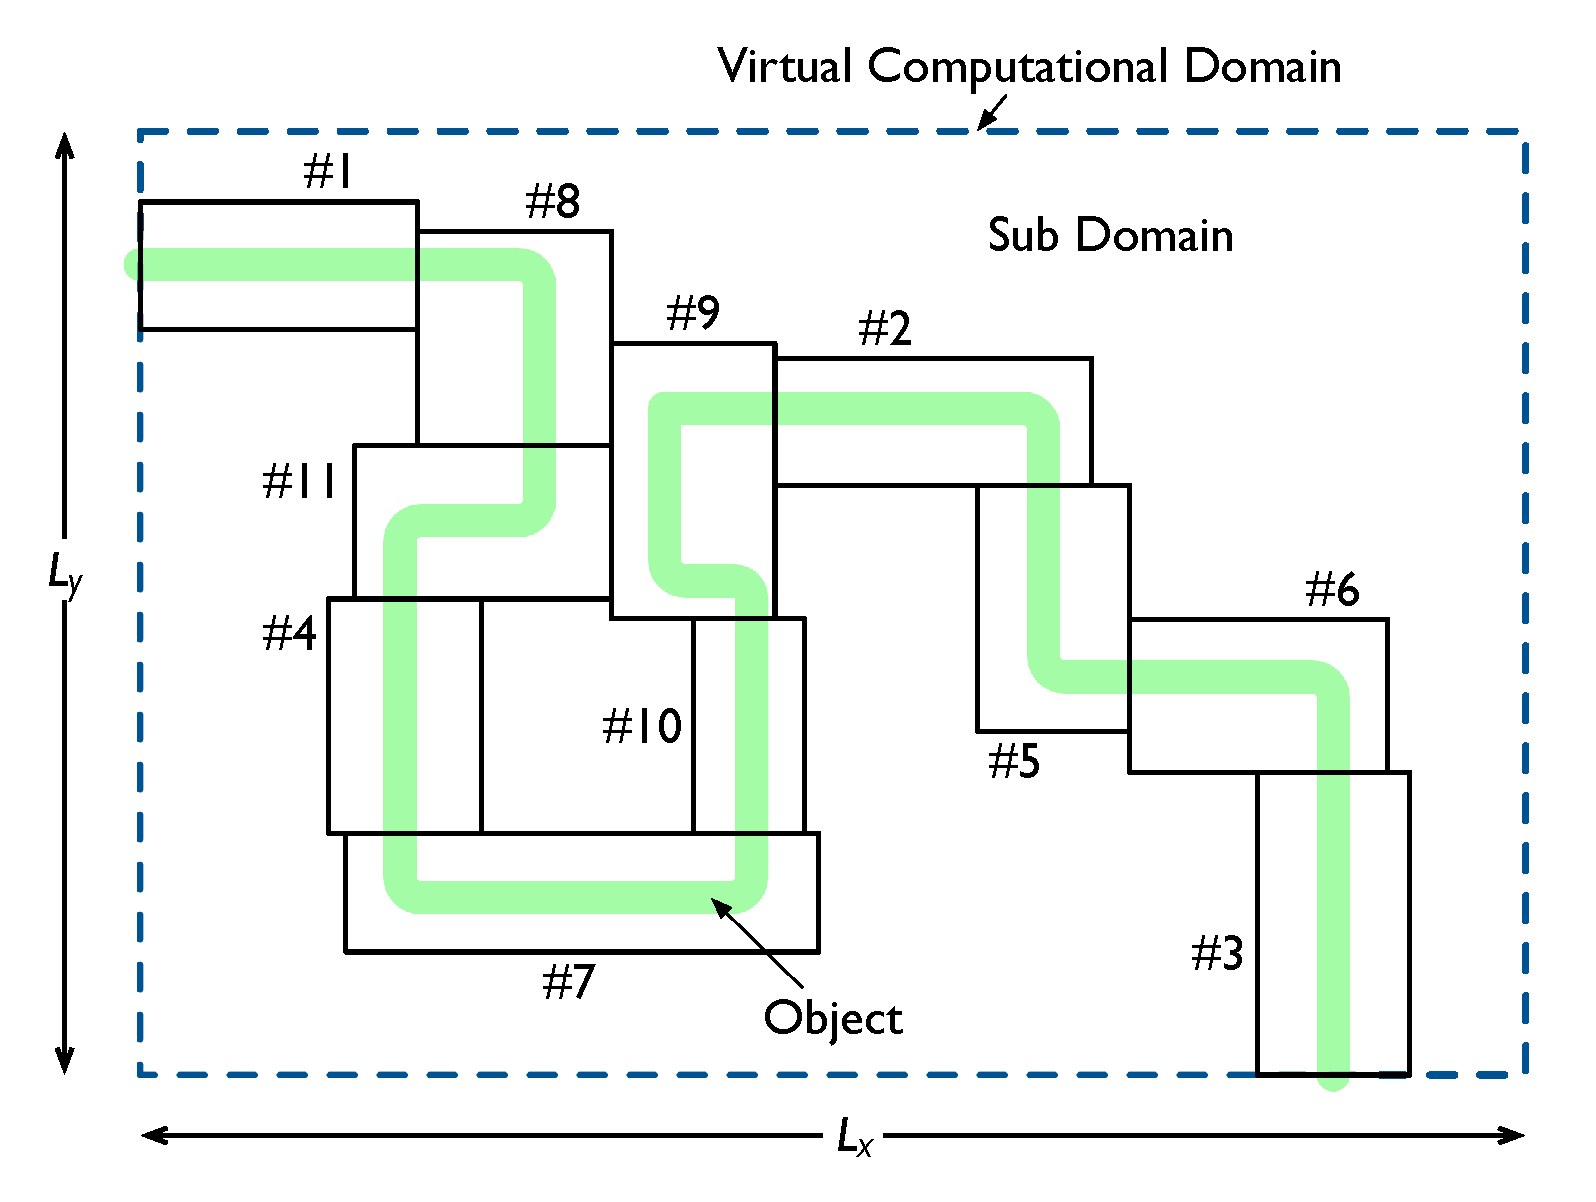
\includegraphics[width=12cm,clip]{mBox.eps}
\end{center}
\caption{Schematic of Multiply-Connected Partitioning}
\label{fig:multibox}
\end{figure}

以下に,マルチボックス計算の手順を示します.
\begin{enumerate}
\item ボクセル生成 V-Xgenを用いてsbxフォーマットのボクセルファイルを作成します.
\item マルチボックスツール sphMbxTool\footnote{09\_Multibox.pdfを参照}を用いて分割ファイルを作成します.
\item XMLファイル 分割ファイル情報をDomainInfoセクションのMBXTBLタグに記述します.


{\small
\begin{program}
<DomainInfo>
  <VoxelSize   ix="64" jx="64" kx="64" />
  <VoxelOrigin ox="0.0" oy="0.0" oz="0.0" />
  <VoxelPitch  dx="0.0" dy="0.0" dz="0.0" />
  <Param name="MDMTBL" dtype="STRING" value="xml/medium.xml" />
  <Param name="BCTBL"  dtype="STRING" value="xml/boundary.xml" />
  <Param name="MBXTBL" dtype="STRING" value="xml/multibox.xml">
</DomainInfo>
\end{program}
}


\item 計算実行 \verb|$mpirun -np 8 sphere hoge.xml|
\end{enumerate}


%
\pagebreak
\section{各プラットホームにおける実行}
\label{sec:exec_platforms}

\subsection{RICC}
\label{sec:exec_RICC}
バッチジョブのスクリプトファイル例を示します.

\begin{indentation}{3zw}{0zw}

{\small
\begin{program}
#!/bin/sh

#----- qsub option
#MJS: -mpc
#MJS: -proc 64
#MJS: -thread 1
#MJS: -mem 1200mb
#MJS: -time 24:00:00
#MJS: -eo
#MJS: -rerun Y
#MJS: -cwd
#MJS: -parallel openmpi

#----- FTLcommand
#FTLDIR: $MJS_CWD
#FTL_SUFFIX: off
#FTL_RANK_FORMAT: 3
#FTL_NO_RANK: off
#
#<BEFORE>
#ALL: sphere_f
#0: P32E_resize_5mm_CutWS.svx
#</BEFORE>
#
#<BEFORE_R>
#ALL: xml
#</BEFORE_R>
#
#<AFTER>
#0: *.sph, *.txt, *.log
#</AFTER>

#----- Program execution
mpirun ./sphere_f xml/p32e.xml
\end{program}
}
\end{indentation}

\pagebreak
次に,利用頻度の高いコマンド類を示します.

\begin{indentation}{3zw}{0zw}
\begin{description}
\item[■] ジョブ投入
{\small
\begin{program}
$ qsub go.sh
\end{program}}

\item[■] ジョブ状態表示
{\small
\begin{program}
$ qstat -m  使用メモリ量
$ qstat -p  プライオリティ
$ qstat -w  実行待ち理由の表示
\end{program}}

\item[■] 実行中Jobの標準出力表示
{\small
\begin{program}
$ qcat REQID
\end{program}}

\item[■] Job優先度変更
{\small
\begin{program}
$ qalter -p <PRIORITY> <REQID>
\end{program}}

\item[■] mpcの計算ノード上のファイル一覧
{\small
OPTIONはlsコマンドと同じである.
\begin{program}
$ qls REQID[@RankID] [OPTION]
\end{program}}

\item[■] mpcの計算ノード上のファイルを取得します.
{\small
\begin{program}
$ qget REQID[@RankID] file
\end{program}}

\end{description}
\end{indentation}





%%%
\chapter{アップデート情報}
\label{chpt:update}
\begin{abstract}
本ユーザガイドのアップデート情報について記します.
\end{abstract}
%
%\section{Update}
{ \small

%
\subparagraph{Version 1.1.9\hspace{1cm}2011/11/7}

\begin{description}
\begin{indentation}{3zw}{0zw}
\item[-] {}~\hyperlink{tgt:average_option}{時間平均パラメータ}の記述を修正しました.
\end{indentation}
\end{description}

\vspace{3mm}

%
\subparagraph{Version 1.1.8\hspace{1cm}2011/9/19}

\begin{description}
\begin{indentation}{3zw}{0zw}
\item[-] 距離情報を用いたスキームの導入に伴い,\hyperlink{tgt:solver_property}{形状近似度}と\hyperlink{tgt:intrinsic model}{IP\_Polygon}のパラメータを追加しました.
\end{indentation}
\end{description}

\vspace{3mm}

%
\subparagraph{Version 1.1.7\hspace{1cm}2011/9/6}

\begin{description}
\begin{indentation}{3zw}{0zw}
\item[-] 表\ref{tbl:intrinsic problems}のPPLT2DのキーワードをParallel\_Plate\_2Dに変更しました.
\item[-] 組み込みモデルのIOP\_Ductクラスの説明を追加しました.
\end{indentation}
\end{description}

\vspace{3mm}

%
\subparagraph{Version 1.1.6\hspace{1cm}2011/9/5}

\begin{description}
\begin{indentation}{3zw}{0zw}
\item[-] 組み込みモデルにCYLINDER, STEPクラスを追加しました.
\end{indentation}
\end{description}

\vspace{3mm}

%
\subparagraph{Version 1.1.5\hspace{1cm}2011/8/31}

\begin{description}
\begin{indentation}{3zw}{0zw}
\item[-] 組み込み例題を\hyperlink{tgt:intrinsic model}{組み込みモデル}として再編集し,\ref{chpt:solver}章の一部の内容を統合しました.
\item[-] 組み込みモデルにPPLT2Dクラスの説明を追加しました.
\end{indentation}
\end{description}

\vspace{3mm}

%
\subparagraph{Version 1.1.4\hspace{1cm}2011/7/28}

\begin{description}
\begin{indentation}{3zw}{0zw}
\item[-] 温度計算時,各媒質に対して\hyperlink{tgt:initial_temp}{初期温度を指定}できるようにしました.
\end{indentation}
\end{description}

\vspace{3mm}

%
\subparagraph{Version 1.1.3\hspace{1cm}2011/7/21}

\begin{description}
\begin{indentation}{3zw}{0zw}
\item[-] 外部領域面の流出境界条件を修正しました.
\end{indentation}
\end{description}

\vspace{3mm}

%
\subparagraph{Version 1.1.2\hspace{1cm}2011/7/11}

\begin{description}
\begin{indentation}{3zw}{0zw}
\item[-] automakeの環境が異なる場合の対応を追記しました.
\item[-] V-Sphereの倍精度と並列モジュールのオプション記述を追加しました.
\item[-] モデル作成に媒質数の制限について加筆しました.
\end{indentation}
\end{description}

\vspace{3mm}

%
\subparagraph{Version 1.1.1\hspace{1cm}2011/7/9}

\begin{description}
\begin{indentation}{3zw}{0zw}
\item[-] CBC Ver. 1.3.6対応
\item[-] 内部境界条件の設定方法を固体セルをキーIDとする方法に変更しました.
\end{indentation}
\end{description}

\vspace{3mm}

%
\subparagraph{Version 1.1.0\hspace{1cm}2011/6/30}

\begin{description}
\begin{indentation}{3zw}{0zw}
\item[-] 外部境界条件と内部境界条件の\hyperlink{tgt:BC policy}{ポリシ}を明示しました.
\item[-] 内部境界条件の注意事項を追記しました.
\end{indentation}
\end{description}

\vspace{3mm}

%
\subparagraph{Version 1.0.9\hspace{1cm}2011/6/21}

\begin{description}
\begin{indentation}{3zw}{0zw}
\item[-] 体裁を変更しました.
\item[-] インストールの章に,\hyperlink{tgt:win_compile}{Windows}でのコンパイルと\hyperlink{tgt:win_opmi_binary}{OpenMPIバイナリパッケージ}を用いたコンパイルを追記しました.
\item[-] 熱境界条件について,\hyperlink{tgt:spec of heat bc}{指定方法}のポリシを追加しました.
\end{indentation}
\end{description}

\vspace{3mm}

%
\subparagraph{Version 1.0.8\hspace{1cm}2011/6/8}

\begin{description}
\begin{indentation}{3zw}{0zw}
\item[-] 境界条件のセクションの構成を変更しました.
\item[-] 熱境界条件を加筆しました.
\end{indentation}
\end{description}

\vspace{3mm}

%
\subparagraph{Version 1.0.7\hspace{1cm}2011/4/11}

\begin{description}
\begin{indentation}{3zw}{0zw}
\item[-] 組み込み例題クラスの\hyperlink{tgt:intrinsic model}{解析モデル}を追記しました.
\end{indentation}
\end{description}

\vspace{3mm}

%
\subparagraph{Version 1.0.6\hspace{1cm}2011/2/11}

\begin{description}
\begin{indentation}{3zw}{0zw}
\item[-] サンプリングのファイル指定を\hyperlink{tgt:monitor_list}{Monitor\_List}に移動しました.
\end{indentation}
\end{description}

\vspace{3mm}

%
\subparagraph{Version 1.0.5\hspace{1cm}2011/1/6}

\begin{description}
\begin{indentation}{3zw}{0zw}
\item[-] 時間平均操作\hyperlink{tgt:average_option}{Average\_Option}のXMLパラメータ書式を変更しました.
\item[-] ファイル入出力\hyperlink{tgt:fileio}{File\_IO}のXMLパラメータ書式を変更しました.
\item[-] 入力ファイル\hyperlink{tgt:input_data}{InputData}のXMLパラメータ書式を変更しました.
\item[-] インターバルのXMLパラメータ指定をFile\_IOとLogセクションに移動しました.
\item[-] 反復パラメータ\hyperlink{tgt:iteration}{Iteration}に温度の反復パラメータを追加しました.
\item[-] ログ出力\hyperlink{tgt:log}{Log}のXMLパラメータ書式を変更しました.
\item[-] モニター指定\hyperlink{tgt:monitor_list}{Monitor\_List}のXMLパラメータ書式を変更しました.
\item[-] 時間制御指定\hyperlink{tgt:time_control}{Time\_Control}のXMLパラメータ書式を変更しました.
\item[-] 単位指定\hyperlink{tgt:unit}{Unit}のXMLパラメータ書式を変更しました.
\item[-] 第\ref{chpt:BC}章の境界条件を変更しました.
\item[-] 第\ref{chpt:monitor}章のXMLパラメータ書式を変更しました.
\item[-] 第\ref{chpt:solver}章を変更しました.
\end{indentation}
\end{description}

\vspace{3mm}

%
\subparagraph{Version 1.0.4\hspace{1cm}2010/12/22}

\begin{description}
\begin{indentation}{3zw}{0zw}
\item[-] パラメータ\hyperlink{tgt:external forcce}{外力項を用いた境界条件}を追加しました.
\item[-] 例題にSHC1Dを追加しました.
\item[-] 解法\hyperlink{tgt:algorithm}{アルゴリズム}に温度の陽解法と陰解法を追加,関連する変更を\hyperlink{tgt:iteration}{Iteration}にも行いました.
\item[-] 対流項スキームの\hyperlink{tgt:convection_term}{O3\_MUSCL}選択時に,minmodリミターを追加しました.
\item[-] ファイル出力指定に\hyperlink{tgt:fileio}{Debug\_Divergence}を追加しました.
\item[-] 内部境界に\hyperlink{tgt:inactive}{不活性境界条件}を追加しました.
\item[-] バージョン情報\hyperlink{tgt:version}{Version\_Info}の記述を変更しました.
\item[-] 分割方法について,\hypertarget{tgt:voxel_division}{VoxelDivisionMethod}を加筆しました.
\item[-] 第\ref{chpt:monitor}章のモニタリング機能を追加しました.また,\hyperlink{tgt:monitor_list}{Monitor\_List}を修正しました.
\end{indentation}
\end{description}

\vspace{3mm}

%
\subparagraph{Version 1.0.3\hspace{1cm}2010/12/7}

\begin{description}
\begin{indentation}{3zw}{0zw}
\item[-] 対流項指定のパラメータ\hyperlink{tgt:convection_term}{Convection\_Term}にO2\_Centralを追加しました.
\item[-] 組み込み例題に\hyperlink{tgt:example}{固体熱伝導}(SHC1D)を追加しました.
\item[-] ログ出力\hyperlink{tgt:log}{Log}で,性能プロファイリング出力に詳細レベルを追加しました.
\item[-] 出力ファイル\hyperlink{tgt:output_data}{OutputData}とログ出力\hyperlink{tgt:log}{Log}に壁面情報出力を追加しました.また,出力ファイルの種類を追加しました.
\item[-] Solver\_Propertyにおいて,\hyperlink{tgt:solver_property}{PDE\_type}の表を追加しました.また,定常/非定常の種別のキーワードをTime\_Variationに変更しました.
\item[-] 並列計算時のボクセル分割の指定方法\hyperlink{tgt:voxel_division}{VoxelDivisionMethod}の説明を追加しました.
\item[-] 外部境界条件の指定方法を変更しました.
\end{indentation}
\end{description}

\vspace{3mm}

%
\subparagraph{Version 1.0.2\hspace{1cm}2010/11/16}

\begin{description}
\begin{indentation}{3zw}{0zw}
\item[-] V-Sphere 1.8.2に対応
\item[-] パラメータInterval,\hyperlink{tgt:log}{Log},\hyperlink{tgt:reference_frame}{Reference\_Frame},\hyperlink{tgt:time_control}{Time\_Control}の指定方法を変更しました.
\item[-] パラメータ\hyperlink{tgt:iteration}{Iteration},\hyperlink{tgt:version}{Version}の表記を修正しました.
\item[-] 境界条件\hyperlink{tgt:preriodic}{周期境界}の指定方法を変更しました.
\end{indentation}
\end{description}

\vspace{3mm}

%
\subparagraph{Version 1.0.1\hspace{1cm}2010/11/1}

\begin{description}
\begin{indentation}{3zw}{0zw}
\item[-] パラメータに\hyperlink{tgt:log}{Log}の説明を追記しました.
\item[-] パラメータの\hyperlink{tgt:interval}{Interval}と\hyperlink{tgt:time_control}{Time\_Control}の時刻指定について,StepとTimeによる指定を排他的にしました.
\item[-] CBCソルバークラスの\hyperlink{tgt:installCBC}{インストール}のセクションで,ディレクトリ構成の変更とdoxygenファイルについて追記しました.
\end{indentation}
\end{description}

\vspace{3mm}

%
\subparagraph{Version 1.0.0\hspace{1cm}2010/10/9}

\begin{description}
\begin{indentation}{3zw}{0zw}
\item[-] ユーザガイド(本編:cbc\_UG.pdf)と内部情報(Inside\_CBC.pdf)を分離しました.
\end{indentation}
\end{description}

} % end of small


%
\bibliographystyle{junsrt}
\bibliography{cbc_UG}

\newpage
\printindex
%
%
\end{document}